%\usepackage{latexsym}
%\usepackage{amsfonts}
%\usepackage{epsfig}
%\usepackage[pdftex]{hyperref}
%\usepackage{fancyhdr}
%\usepackage{toptesi}
%\usepackage{listings}
%\lstloadlanguages{C++}

%\usepackage{caption}
%\usepackage{psfrag}
%\usepackage{booktabs}
%\usepackage[numbers]{natbib}

%\documentclass[12pt,twoside]{toptesi}

\documentclass[12pt,oneside]{toptesi}

\usepackage{epstopdf}
\usepackage{amsmath}
\usepackage{amssymb}
\usepackage{graphicx}
\usepackage{epsfig}
\usepackage{subfigure}

\pdfinfo{
  /Title    (Implementation of an object oriented parallel code to solve the problem of plasma equilibrium in a mirror machine using a spectral element method)
  /Author   (Marco Agnese)
  /Creator  ()
  /Producer ()
  /Subject  (Applied Mathematics)
  /Keywords (spectral element methods, mirror machine, plasma equilibrium, C++, parallel computing)
}

\begin{document}
\english

\begin{titlepage}
\centerline{\LARGE POLITECNICO DI TORINO}
\bigskip
\vspace{1cm}
\centerline{\LARGE I Facolt\`a di Ingegneria}
\centerline{Corso di Laurea Specialistica in Ingegneria Matematica}
\vspace{0.8cm}
\centerline{

\includegraphics[width=3cm,angle=0]{images/MarchioPoli.pdf}}
\vspace{0.8cm}

\centerline{\Large\bfseries\sf Master thesis}
\vspace{0.5cm}
\begin{center}
\textbf{{\LARGE\bfseries Implementation of an object oriented parallel code to solve the problem of plasma equilibrium in a mirror machine using a spectral element method}\\}
\vspace{0.5cm}
\end{center}
\begin{center}
\bfseries\sf\large{Marco Agnese}
\end{center}
\vspace{0.7cm}
\begin{minipage}[t]{0.4\textwidth}
\centering
\textit{Advisors:}\\
\vspace{0.7cm}
{Prof. Nicola \textsc{Bellomo} }\\
\vspace{0.7cm}
{Prof. Gianni \textsc{Coppa} }\\
\vspace{0.7cm}
{Prof. Luca \textsc{Formaggia} }\\
\end{minipage}
\hfill
\begin{minipage}[t]{0.47\textwidth}
\centering
\textit{Internship supervisors:}\\
\vspace{0.7cm}
{Dr. Zehua \textsc{Guo } }\\
\vspace{0.7cm}
{Dr. Xianzhu \textsc{Tang } }\\
\end{minipage}
\vfill
\vspace{1cm}
\centerline{July 2013}
\end{titlepage}

\thispagestyle{empty}
~\\
Prof. \emph{Nicola Bellomo}\\
Department of Mathematics,\\
Politecnico di Torino,\\
Corso Duca degli Abruzzi 24,\\
10129 Torino, Italy\\
~\\
~\\
Prof. \emph{Gianni Coppa}\\
Department of Energetics,\\
Politecnico di Torino,\\
Corso Duca degli Abruzzi 24,\\
10129 Torino, Italy\\
~\\
~\\
Prof. \emph{Luca Formaggia}\\
Department of Mathematics,\\
Politecnico di Milano,\\
Via Bonardi 9,\\
20133 Milano, Italy\\
~\\
~\\
~\\
~\\
~\\
~\\
~\\
~\\
~\\
~\\
~\\
~\\
Dr. \emph{Zehua Guo}\\
Applied Mathematics and Plasma Physics,\\
MS K717 - Los Alamos National Laboratory,\\
Los Alamos, NM 87545, USA
~\\
~\\
Dr. \emph{Xianzhu Tang}\\
Applied Mathematics and Plasma Physics,\\
MS B268 - Los Alamos National Laboratory,\\
Los Alamos, NM 87545, USA


\tableofcontents

\chapter*{Acknowledgements}
\addcontentsline{toc}{chapter}{Acknowledgements}

I would like to express my gratitude to all those who gave me the possibility to complete this thesis.

I am grateful to Los Alamos National Laboratory for the great opportunity which has been offered to me and the Department of Energy of United States of America who supported this work. In particular, I would like to gratefully acknowledge the assistance of Dr G. Delzanno, Dr Z. Guo and Dr X. Tang from LANL whose help, suggestions and encouragement helped me to accomplish this work.

I also want to thank my advisors Prof. N. Bellomo, Prof. G. Coppa and Prof. L. Formaggia for all their support.
\medskip

I want to express a great gratitude to my mother, my father and Alessandro which have always supported me and believed in me.

A special thanks to my ``second brother'', Ivan, and Federica for their friendship.

I want to thank Francesco and Marco who helped me to survive 11 months in the middle of nowhere, without them Los Alamos would have been very boring, and Lorenzo for the five years spent together at the Politecnico.

Finally, I want to thank Silvia who has been very patient for almost one year; she helped me to prove that the ``Los Alamos curse'' can be defeated.


\chapter*{Abstract}
\addcontentsline{toc}{chapter}{Abstract}
LAPS is a multi-physics plasma simulation framework and code suite which provides data structures and communication infrastructure on massively parallel computers. It leverages heavily on existing parallel solvers provided by or through \verb|PETSc|. A key module of LAPS is the plasma equilibrium solver for both axisymmetric linear and toroidal configurations, with closed flux surfaces or with boundary intercepting open field lines, using the generalized Grad-Shafranov equation, which is a nonlinear elliptic partial differential equation. By the assumption of axisymmetry, the equilibrium solver concerns only two spatial dimensions.  We have chosen a spectral element method (SEM) with a modal basis and Gaussian integration because it ensures an exponential convergence for smooth solutions, which are expected for plasma equilibrium.

Quadrilateral elements are adopted since it is straightforward to generalize the SEM on the domain $\Omega_1\subset\mathbb{R}$ to the domain $\Omega_2\subset\mathbb{R}^2$ using a basis tensor product. We adopt unstructured instead of commonly used structured mesh for quadrilateral elements for the reason that open field line equilibrium at the tokamak edge requires nontrivial multi-block meshing around the X point. An object oriented generic code is written using \verb|C++|. It reads an unstructured mesh created with \verb|GMSH| and makes an optimal partitioning among the processes. The SEM discretized problem is then solved using the \verb|PETSc| library. Instead of solving directly the system of equations, we rewrite the stiffness matrix with the static condensation technique splitting the contribution of the interior modes and edge modes in order to reduce the communication among the processors to maximize the parallelization of the code and the performance.

In our initial implementation, the equilibrium is solved in the domain delimited by the magnetic field generated by the device. Later it will be solved in the entire physical geometry which leads to a free boundary problem since it is unknown an a priori plasma/vacuum interface. A further development of the code will be the implementation of a common interface which will allow the exchange of the results obtained with different methods of LAPS in order to increase the flexibility and an h-p adaptivity for the code to improve the quality of the solution and the order of convergence of the method.


\chapter*{Sommario}
\addcontentsline{toc}{chapter}{Sommario}
Il LAPS \`{e} un framework per simulazioni multifisiche di plasmi che offre strutture di dati e infrastrutture di comunicazione per grandi cluster di computers paralleli; per fare ci\`{o} esso utilizza ampiamente i solutori paralleli forniti da o attraverso la libreria \verb|PETSc|. Un modulo fondamentale del LAPS \`{e} il solutore per studiare l'equilibrio del plasma sia in configurazioni toroidali, sia in configurazioni con simmetria assiale, risolvendo l'equazione non lineare alle derivate parziali conosciuta come equazione di Grad-Shafranov generalizzata. Grazie all'ipotesi di simmetria assiale, il solutore di equlibrio opera utilizzando solamente due coordinate spaziali. Il metodo numerico scelto \`{e} un metodo agli elementi spettrali (SEM) con una base modale e con integrazione Gaussiana; tale metodo assicura una convergenza esponenziale quando la soluzione \`{e} regolare, fatto altamente probabile traddandosi di un problema d'equlibrio.

Per la discretizzazione del dominio abbiamo adottato una mesh non strutturata con elementi quadrangolari; questa scelta \`{e} stata dettata dal fatto che \`{e} abbastanza semplice generalizzare un metodo SEM da un dominio $\Omega_1\subset\mathbb{R}$ ad un dominio $\Omega_2\subset\mathbb{R}^2$. L'utilizzo di mesh non strutturate dipende invece dal fatto che in un tokamak le linee aperte d'equilibrio richiedono un complicato meshing multiblocco intorno all'X-point. Abbiamo scritto un codice \verb|C++| generico orientato agli oggetti che legge una mesh non strutturata creata con il software \verb|GMSH| e performa un partizionamento ottimale tra i processi. Il problema discretizzato \`{e} poi risolto utilizzando la libreria \verb|PETSc|; tuttavia, invece di risolvere il sistema lineare direttamente, riscriviamo la matrice di rigidezza usando la static condensation technique che consiste nel separare i contributi dei modi interni da quelli esterni riducendo la comunicazione tra i processi. Ci\`{o} massimizza la parallelizzazione del codice e ne aumenta le performance.

Inizialmente l'equilibrio \`{e} risolto in un dominio delimitato dal campo magnetico generato dalla macchina ma in seguito sar\`{a} risolto in tutta la geometria fisica originando un problema di free boundary dato che non si conosce a priori l'interfaccia plasma/vuoto. Un ulteriore sviluppo del codice sar\`{a} l'implementazione di un'interfaccia comune la quale permetter\`{a} lo scambio di risultati ottenuti dalle differenti parti del LAPS per aumentarne la flessibilit\`{a} ed un adattivit\`{a} h-p per migliorare la qualit\`{a} della soluzione e l'ordine di convergenza del metodo.


\chapter{MHD equilibrium problem}\label{chapter:GS}
In this chapter, after a short introduction where we summarize what is a plasma and the differences way to confine it, we focus our attention to the mirror machine, which is a particular configurations for confinement, describing the physical principle behind that: the conservation of magnetic moment. Finally, starting from a fluid model, we derive the equilibrium equation for a plasma confined by the mirror device.

\section{Introduction}\label{sec:introduction}
Plasma is one of the four fundamental states of matter which consists in an ionized gas. More precisely it is a high-temperature collection of independently moving charged particles, ions and electrons, dominated by electromagnetic forces. Ionization can be induced by heating a gas or by strong electromagnetic field applied with a laser or microwave generator. The presence of a non-negligible number of charge carriers makes the plasma electrically conductive so that it responds strongly to electromagnetic fields. The motion depends not only on local conditions, but on the state of plasma in remote regions as well, because elements of plasma exert a force on one another even at large distances. In fact the motion of local concentrations of charged particles, which give rise to electric field, generates currents and thence a magnetic field that affects the motion of other particles. Cmp. \cite{CHEN}.
\medskip

Criteria for plasma:
\begin{itemize}
  \item $\lambda_D\ll L$ When the Debye length, defined as $\lambda_D=\sqrt{\frac{\epsilon_0 k_B T_e}{n_eq_e^2}}$ is short compared to the physical size L of the plasma, then the plasma is quasineutral. Quasineutral means that the ionized gas is neutral enough so that globally the density of ions is approximatively equals to the density of electrons $n_i\simeq n_e\simeq n$ but locally no so neutral that all the interesting forces vanish. This criterion sets the predominance of interactions in the bulk of plasma over those at its edges, where boundary effects may take place.
  \item $N_D\ll 1$ The plasma approximation is valid when the number of charge carriers within the Debye sphere of influence $N_D=n\frac{4}{3}\pi\lambda_D^3$ of a particular particle is higher than unity to provide collective behavior of the charged particles.
  \item $\omega_{\tau}>1$ When the frequency $\omega$ of typical plasma oscillations is large than the frequency $\frac{1}{\tau}$ of collision with neutral atoms, then electrostatic interactions dominate over the processes of ordinary gas kinetics.
\end{itemize}

Fusion is a form of nuclear energy which consists in the merging of light elements, mainly hydrogen (H) and its isotopes deuterium (D) and tritium (T) to produce energy. To burn D–T one is required to heat it to the astounding temperature of $1.5\cdot 10^6 K$, hotter than the center of the sun. Once heated some method must be devised to hold the plasma together. The primary method requires a clever configuration of magnetic fields.
\medskip

The determination of MHD equilibrium configurations is an integral part of the problem of designing plasma confinement devices. Indeed equilibrium calculations play a major role in reactor studies where a knowledge of the plasma configuration provides the basic framework for detailed system design. The Grad-Shafranov equation is a two dimensional, nonlinear elliptic PDE which describes the relation between the plasma current and the pressure in terms of flux. It provides a complete description of ideal MHD equilibrium.
\medskip

At present, there are two main types of magnetic configurations for plasma confinement: closed (tokamak, stellarator, etc) and open (mirrors). Although closed configurations are more developed, advantages of the open systems could be useful in future for the fusion program. It should be mentioned the most important features of open systems:
\begin{itemize}
  \item most of such systems can operate in steady state regime and, at the same time, effects of disruptions are not appeared in them;
  \item plasma pressure can be comparable with magnetic field pressure;
  \item there are no divertor problems in the mirror case;
  \item open systems are convenient for direct energy conversion of charged particles. This circumstance can turn out to be especially important in a future for low-neutron schemes of fusion reactions.
\end{itemize}

\section{The mirror machine}\label{sec:mirror_machine}
The simplest device designed to confined a plasma is the mirror machine: it leverages the mirror effect to trap plasma particles using magnetic fields. To understand how it works it is necessary to briefly summarize the theory known as \textit{Single-particle motion} which describes the motion of charged of charged particles in prescribed magnetic and electric fields. For a more detailed explanation cmp. \cite{plasma}.

The starting point are the equations of motion as determined from Newton’s law. For plasma physics applications, only the magnetic and electric forces, given by Lorentz force, are required since gravity has a very small effect and can be neglected. The equations to be solved are thus:
\begin{equation}\label{eq:newton}
  \begin{cases}
    m\frac{\mathrm{d}\mathbf{v}}{\mathrm{d}t}=q(\mathbf{E}+\textbf{v}\times{\mathbf{B}})\\
    \frac{\mathrm{d}\mathbf{r}}{\mathrm{d}t}=\mathbf{v}
  \end{cases}
\end{equation}
where $\mathbf{B}=\mathbf{B}(\mathbf{r},t)$ and $\mathbf{E}=\mathbf{E}(\mathbf{r},t)$. The fields are simply specified as known quantities, therefore self-consistency is not taken in account. $\textbf{B}$ and $\textbf{E}$ are assumed to be smooth, slowly varying functions in order to be compatible with the requirement that plasmas be dominated by long-range collective effects.

It is possible to study the motion of a single particle using specific configurations of the two fields in order to solve analytically the model (\ref{eq:newton}); combining all the motions, the general trajectory of a particle is obtained. The mirroring takes place when one of these specific configurations is used.
\medskip

Let's suppose to have the following fields
\begin{equation}\label{eq:fields_magnetic_moment}
  \begin{cases}
    \mathbf{E}_{\perp}=E_x(x,t)\mathbf{e}_y\\
    \mathbf{B}=B(t)\mathbf{e}_z.
  \end{cases}
\end{equation}
Substituting Eq.(\ref{eq:fields_magnetic_moment}) in Eq.(\ref{eq:newton}) it is possible to derive, using some physical considerations, the following simplified system
\begin{equation}\label{eq:newton_simp}
  \begin{cases}
    \frac{\mathrm{d}v_x}{\mathrm{d}t}-\omega_cv_y=0\\
    \frac{\mathrm{d}v_y}{\mathrm{d}t}+\omega_cv_x=\frac{\omega_c}{B}\big(E_y+\frac{\partial E_y}{\partial x_g}(x-x_g)\big)
  \end{cases}
\end{equation}
where $\omega_c=\frac{qB}{m}$ is the gyro frequency and $(x_g,y_g)$ is the center, called guiding center, of the orbit of the circular-type motion described by the charged particle in the prescribed field. The right-hand side of the second equation (\ref{eq:newton_simp}) is a first order expansion around the guiding center. Introducing a new time variable
\begin{equation}
  \tau=\int_0^t\omega_c(t')\:\mathrm{d}t',
\end{equation}
which implies $\mathrm{d}\tau=\omega_c\mathrm{d}t$, we can reduce the model to
\begin{equation}\label{eq:newton_simp_bis}
  \begin{cases}
    \frac{\mathrm{d}v_x}{\mathrm{d}\tau}-v_y=0\\
    \frac{\mathrm{d}v_y}{\mathrm{d}\tau}+v_x=\frac{1}{B}\big(E_y+\frac{\partial E_y}{\partial x_g}(x-x_g)\big)\\
    \frac{{d}x}{\mathrm{d}\tau}=\frac{v_x}{\omega_c}\\
    \frac{{d}y}{\mathrm{d}\tau}=\frac{v_y}{\omega_c}.
  \end{cases}
\end{equation}
We can rewrite $v_x$ and $v_y$ in terms cylindrical velocity coordinates:
\begin{equation}\label{eq:cylindrical_velocities}
  \begin{cases}
    v_x=v_{\perp}(\tau)\cos(\tau+\varepsilon(\tau))+\frac{E_y}{B}\\
    v_y=-v_{\perp}(\tau)\sin(\tau+\varepsilon(\tau))+\frac{\mathrm{d}}{\mathrm{d}\tau}\big(\frac{E_y}{B}\big)
  \end{cases}
\end{equation}
where the variables $v_x$ and $v_y$ have been replaced by new unknowns $v_{\perp}(\tau)$, $\varepsilon(\tau)$. The remainder of the analysis focuses on solving $v_{\perp}(\tau)$ since it gives origin to an approximate constant of the motion. The solution for $\varepsilon(\tau)$ can also be easily found but no new important information is contained therein and hence the corresponding analysis is suppressed. Before substituting Eq.(\ref{eq:cylindrical_velocities}) in Eq.(\ref{eq:newton_simp_bis}) it is necessary to find an expression for the term $x-x_g$; since this expression appears only in the small, expanded term, the leading order gyro motion contribution is all that is required. From the second two trajectory equations in Eq.(\ref{eq:newton_simp_bis}) one finds that
\begin{equation}\label{eq:approx_gyro_coor}
  x-x_g\approx\frac{v_{\perp}(\tau)}{\omega_c(\tau)}\sin(\tau+\varepsilon(\tau)).
\end{equation}
Substituting Eq.(\ref{eq:approx_gyro_coor}) and Eq.(\ref{eq:cylindrical_velocities}) in Eq.(\ref{eq:newton_simp_bis}), solving simultaneously for $\frac{\mathrm{d}v_{\perp}}{\mathrm{d}\tau}$, $\frac{\mathrm{d}\varepsilon}{\mathrm{d}\tau}$ and using Faraday's law $\frac{\partial E_y}{\partial x_g}=-\frac{\mathrm{d}B}{\mathrm{d}t}=-\omega_c\frac{\mathrm{d}B}{\mathrm{d}\tau}$ it is possible to obtain
\begin{equation}\label{eq:magnetic_moment}
  \frac{1}{\mu}\frac{\mathrm{d}\mu}{\mathrm{d}\tau}=\frac{1}{B}\frac{\mathrm{d}B}{\mathrm{d}\tau}\cos 2(\tau+\varepsilon)
\end{equation}
where
\begin{equation}
  \mu=\frac{mv^2_{\perp}}{2B};
\end{equation}
higher order terms have been neglected. The quantity $\mu$ is called \textit{magnetic moment}.
\medskip

The equation (\ref{eq:magnetic_moment}) can be further simplified integrating over one gyro period $\tau_0\leq\tau +\varepsilon\leq(\tau_0+2\pi)$. Indeed one finds that the right hand side almost exactly averages to zero, except for a very small, negligible correction. It follows that $\mu$ is a constant of the motion when averaged over one gyro period since
\begin{equation}
  \langle\frac{\mathrm{d}\ln\mu}{\mathrm{d}\tau}\rangle\approx0\qquad\Longrightarrow\qquad \mu=\mathrm{const}.
\end{equation}
The quantity $\mu$ is  also known as the first adiabatic invariant and is equal to the gyro-averaged magnetic moment of the charged particle. The fact that $\mu$ is constant when averaged over a gyro period can be interpreted as follows. The magnetic flux enclosed by a particle over one gyro orbit is just $\psi=\pi r^2B=\frac{2\pi m}{q^2}\mu\approx\mu$. Therefore, as the B field changes slowly in time the perpendicular velocity and corresponding gyro radius also change slowly in time in such a way that the flux contained within the orbit is a constant.

\begin{figure}
\centering
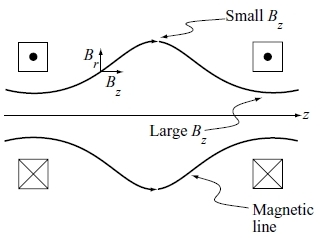
\includegraphics[scale=.6]{images/B_gradient.jpg}
\caption{Coil configuration generating a magnetic field gradient along $z$ direction.}
\label{fig:B_gradient}
\end{figure}

With an approach similar to the one followed before, we can study the effect of a parallel gradient in the magnetic field, which can arise in configurations such as those illustrated in  Fig.(\ref{fig:B_gradient}).The fields configuration in this case is
\begin{equation}\label{eq:fields_mirroring}
  \begin{cases}
    \mathbf{E}=0\\
    \mathbf{B}=B_x(x,z)\mathbf{e}_x+B_z(x,z)\mathbf{e}_z
  \end{cases}
\end{equation}
where, for simplicity, the geometry, Fig.(\ref{fig:B_gradient_slab}), is a slab version of the cylindrical configuration shown in Fig.(\ref{fig:B_gradient}).

\begin{figure}
\centering
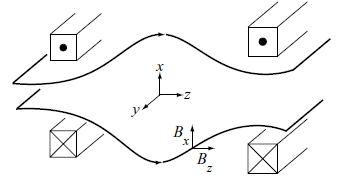
\includegraphics[scale=.6]{images/B_gradient_slab.jpg}
\caption{Slab approximation.}
\label{fig:B_gradient_slab}
\end{figure}

Two important results can be derived in the limit where the gyro radius is small compared to the spatial gradient length of the field. Firstly, the magnetic moment is again an adiabatic invariant but now the time dependency becomes a spatial since, after averaging over a gyro-period, $v_{\perp}=v_{\perp}(z)$ and $B=B(z)$. Secondly, it is possible to find gyro-averaged force acting on the parallel guiding center motion of the particle. The force is driven by the parallel gradient in the magnetic field and has the following expression
\begin{equation}
  m\frac{\mathrm{d}v_{\|}}{\mathrm{d}t}=-\mu\nabla_{\|}B.
\end{equation}

The combination of $\mu=\mathrm{const}$ and $F_{\|}=−\mu\nabla_{\|} B$ can rule the parallel motion of the guiding center. In particular, the direction of the parallel motion can be completely reversed since there is a critical point, called \textit{mirror point}, along the trajectory where the particle is reflected. This reversal process is named \textit{mirror effect}. This process is well described in Fig.(\ref{fig:mirroring}).

\begin{figure}
\centering
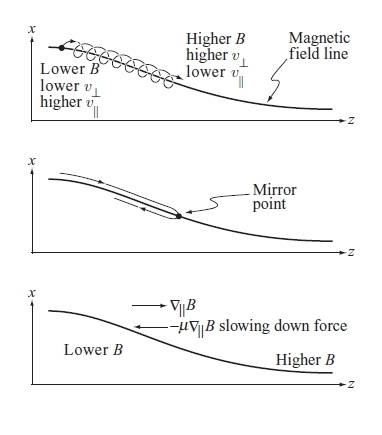
\includegraphics[scale=.6]{images/mirroring.jpg}
\caption{The mirror effect.}
\label{fig:mirroring}
\end{figure}

A particle, with initial velocity $(v_{\|},v_{\perp})$ moves from a region of lower field into the high-field region and the value of $B$ along the guiding center increases. Since $\mu=\frac{mv^2_{\perp}}{2B}=\mathrm{const}$, $v_{\perp}$ must increase and, since in a static magnetic field the kinetic energy of a particle is constant $E=\frac{1}{2}m(v_{\perp}^2+v_{\|}^2)=\mathrm{const}$, $v_{\|}$ must decrease. Therefore, if $B$ increases sufficiently, the particle reaches a point along its trajectory where $v_{\|}=0$: the reflection point. Once reflected, the parallel velocity of the particle reverses direction and the guiding center motion starts moving to the left. The force causing this behavior is $F_{\|}$.

\begin{figure}
\centering
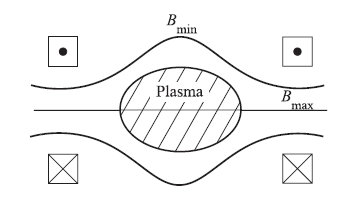
\includegraphics[scale=.6]{images/mirror_machine.jpg}
\caption{Geometry of the simplest mirror machine.}
\label{fig:mirror_machine}
\end{figure}

The mirror effect is the physical principle used to confine plasma in the earliest magnetic fusion configurations: the \textit{mirror machine}, cmp. Fig.(\ref{fig:mirror_machine}). This device simply consists of two coils with currents flowing in the same direction which create a magnetic field with a maximum just under each coil and a local minimum midway between. Using the guiding center theory, it is simple to evaluate that a large fraction of the particles remain confined. Unfortunately practical experiments have shown that the simple mirror machine did not work as well as predicted since macroscopic and microscopic instabilities were observed, leading to anomalously fast losses of particles at the extreme points of the device. Indeed Coulomb collisions scatter many particles to very high parallel velocity and these particles escape from the device.

\section{Grad-Shavranov equation}\label{sec:grad_shavranov}
The densities of plasmas are such that they belong to an intermediate range between fluids and a collection of individual particles. Under appropriate hypothesis the identity of individual particle is negligible and only the motion of conducting fluids is taken into account, so we can study the plasma confinement in the mirror machine within the ideal magnetohydrodynamics (MHD) which is a single-fluid model. The MHD model is a reduction of the two-fluid model, where ions and electrons are described like two fluids by conservation equations coupled with Maxwell's equations, derived by focusing attention on the length and time scales characteristic of macroscopic behavior. For more details cmp. \cite{GUO}, \cite{plasma} and \cite{idealMHD}. The explicit computations are reported in Appendix.
\medskip

The MHD equilibrium model is
\begin{subequations}\label{eq:MHD_equlibrium}
  \begin{align}
    \label{eq:MHD_momentum}\mathbf{J}\times\mathbf{B}&=\nabla\cdot\mathbb{P}\\
    \label{eq:MHD_current}\nabla\times\mathbf{B}&=\mathbf{J}\\
    \label{eq:MHD_maxwell}\nabla\cdot\mathbf{B}&=0
  \end{align}
\end{subequations}
where $\mathbf{B}$ is the magnetic field, $\mathbf{J}$ is the plasma current and $\mathbb{P}$ is the gyrotropic pressure tensor defined as
\begin{equation}\label{eq:pressure_tensor}
  \mathbb{P}=p_\perp\mathbb{I}+(p_\parallel - p_\perp)\mathbf{b}\otimes\mathbf{b}.
\end{equation}

The vector $\mathbf{b}=\frac{\mathbf{B}}{B}$ is the unit vector parallel to $\mathbf{B}$ and $B=\|\mathbf{B}\|$ is the magnitude of the magnetic field; the scalar components $p_\perp$ and $p_\parallel$ are definable in terms of a distribution function $g_0$ of guiding centers , cmp. \cite[p. 1614]{magnetic_mirror}, as
\begin{equation}\label{eq:pressure_components}
  p_\perp=\int g_0\,v^2_\perp \mathrm{d}^3 v \quad\mbox{and}\quad p_\parallel=\int g_0\,v^2_\parallel \mathrm{d}^3 v
\end{equation}
where $v_\perp$ and $v_\parallel$ are the component of fluid velocity perpendicular and parallel to the magnetic field, respectively, and
$\mathrm{d}^3 v=\mathrm{d}v_\perp\mathrm{d}v_\parallel\mathrm{d}\phi$.

Equation (\ref{eq:MHD_current}) is the Ampere law while (\ref{eq:MHD_maxwell}) represents the conservation of magnetic flow; equation (\ref{eq:MHD_momentum}) establishes that at the equilibrium there is a balance force between force due to the pressure and Lorentz force $\mathbf{J}\times\mathbf{B}$.
\medskip

Taking the divergence of (\ref{eq:pressure_tensor}) and introducing the magnetic field-line curvature vector $\mathbf{k}=\mathbf{b}\cdot\nabla\mathbf{b}=(\nabla\times\mathbf{b})\times\mathbf{b}$, we obtain
\begin{equation}\label{eq:div_press}
  \nabla\cdot\mathbb{P}=\nabla p_\perp+(p_\parallel - p_\perp)\mathbf{k}+\left[\mathbf{b}\cdot\nabla(p_\parallel - p_\perp)-
  \frac{1}{B}(p_\parallel - p_\perp)\nabla B\cdot\mathbf{b}\right]\mathbf{b}
\end{equation}
  and taking the dot product between (\ref{eq:div_press}) and $\mathbf{b}$, we find the relation between $p_\perp$ and $p_\parallel$ along the magnetic field
\begin{equation}\label{eq:pressure_balance}
  p_\perp=p_\parallel-B\frac{\partial p_\parallel}{\partial B}.
\end{equation}

This relation replaces the simple condition $\mathbf{b}\cdot\nabla p=0$ of the isotropic scalar pressure theory. The longitudinal pressure balance equation states that only if $p_\perp>p_\parallel$ it is possible to balance the plasma pressure $p_\parallel$ using a positive gradient of $\mathbf{B}$.

Moreover we can find the expression for the parallel and perpendicular components of the plasma current respect to the magnetic field. From Eq.(\ref{eq:MHD_momentum}) we have
\begin{equation}
  \mathbf{B}\times\mathbf{J}\times\mathbf{B}=\mathbf{B}\times\nabla\cdot\mathbb{P}
\end{equation}
but
\begin{equation}
  \mathbf{B}\times\mathbf{J}\times\mathbf{B}=(\mathbf{B}\cdot\mathbf{B})\mathbf{J}-(\mathbf{B}\cdot\mathbf{J})\mathbf{B}=B^2\mathbf{J}-(\mathbf{B}\cdot\mathbf{J})\mathbf{B}
\end{equation}
so
\begin{equation}\label{eq:current_comp}
  \mathbf{J}=\frac{1}{B^2}(\mathbf{B}\cdot\mathbf{J})\mathbf{B}+\frac{1}{B^2}\mathbf{B}\times\nabla\cdot\mathbb{P}=
  (\mathbf{b}\cdot\mathbf{J})\mathbf{b}+\frac{1}{B}\mathbf{b}\times\nabla\cdot\mathbb{P}=\mathbf{J}_\parallel+\mathbf{J}_\perp
\end{equation}
\medskip

It is convenient to rewrite the system of equations (\ref{eq:MHD_equlibrium}) using the Clebsch coordinates $(\psi,\theta,\phi)$ or flux coordinates, cmp. \cite{fluxcoord}. To do that, firstly we define flux surface a smooth surface $S$ with normal $\textbf{n}$ such that $\mathbf{B}\cdot\mathbf{n}=0$ everywhere on $S$ which implies that the magnetic field does not cross $S$ anywhere.  It is then possible to define a scalar flux function $\psi$ such that its value is constant on $S$, and $\mathbf{B}\cdot\nabla \psi=0$. Assuming the flux surfaces have a toroidal topology, the function $\psi$ defines a set of nested surfaces, so it makes sense to use this function to label the flux surfaces, i.e., $\psi$ may be used as a "radial" coordinate. Each toroidal surface $\psi$ encloses a volume $V(\psi)$ and the surface corresponding to an infinitesimal volume is essentially a line which corresponds to the toroidal axis.

From (\ref{eq:MHD_maxwell}) it follows that $\mathbf{B}$ can be rewritten as
\begin{equation}
  \mathbf{B}=\nabla\times\mathbf{A}=\nabla\times(\alpha\nabla\beta)=\nabla\alpha\times\nabla\beta.
\end{equation}
The flux of $\mathbf{B}$ through a surface $S$ with unit normal vector $\mathbf{n}$ outward from the volume $V$, enclosed by $S$, is
\begin{equation}
  \int_S\mathbf{B}\cdot\mathrm{d}\mathbf{S}=\int_S(\nabla\times(\alpha\nabla\beta))\cdot\mathrm{d}\mathbf{S}=\oint_l\alpha\nabla\beta\cdot\mathrm{d}\mathbf{l}=\oint_l \alpha\mathrm{d}\beta;
\end{equation}
choosing $\alpha=\psi$ and $\beta=\theta$ we obtain
\begin{equation}\label{eq:clebsch}
  \mathbf{B}=\nabla\psi\times\nabla\theta
\end{equation}
end
\begin{equation}
 \int_S\mathbf{B}\cdot\mathrm{d}\mathbf{S}=\int_0^{2\pi} \psi\mathrm{d}\theta=2\pi\psi.
\end{equation}

Therefore, except for a proportionality constant, the coordinate $\psi$ measures the total magnetic flux enclosed within a constant $\psi$ surface. Instead $\theta$ is orthogonal to $\psi$ and it is $2\pi$-periodic angle-like on each flux surface. Finally let's call $\phi$ the distance along a field line, cmp. \cite[p. 1617]{magnetic_mirror}. Moreover $\mathbf{b}\cdot\nabla\psi=0$ and $\mathbf{b}\cdot\nabla\theta=0$ which means that $\psi$ and $\theta$ remain constant along field lines, but its value may vary from one filed line to another. In particular $\psi=\mathrm{const}$ define the axial flux surfaces upon which the trapped particle guiding centers move: it can be used to plot the trajectories of particles in the steady flow.
\medskip

Using the Clebsch coordinates it is possible to rewrite the system of equation (\ref{eq:MHD_equlibrium}) like an unique equilibrium equation in that reference frame but, for our purposes, it is better to choose a cylindric coordinates set $(r,\theta, z)$. Under the axisymmetric hypothesis, which means that $z$ is an axis of revolution and $\frac{\partial(\cdot)}{\partial \theta}=0$, the magnetic field is independent of the angular coordinate $\theta$. So $\psi=\psi(r,z)$ and its gradient can be written as
\begin{equation}
  \nabla\psi=\frac{\partial\psi}{\partial r}\nabla r+\frac{\partial\psi}{\partial z}\nabla z
\end{equation}
and (\ref{eq:clebsch}) becomes
\begin{equation}
  \mathbf{B}= \frac{\partial\psi}{\partial r}\nabla r \times\nabla\theta+\frac{\partial\psi}{\partial z}\nabla z \times\nabla\theta
\end{equation}
or in the covariant basis $(\mathbf{e}_r,\mathbf{e}_\theta,\mathbf{e}_z)$, where $\mathbf{e}_\theta=r\nabla\theta$,
\begin{equation}\label{eq:covariantB}
 \mathbf{B}=-\frac{1}{r}\frac{\partial\psi}{\partial z}\mathbf{e}_r+\frac{1}{r}\frac{\partial\psi}{\partial r}\mathbf{e}_z.
\end{equation}

From (\ref{eq:covariantB}) and (\ref{eq:MHD_current}) we obtain the current in contravariant components
\begin{equation}\label{eq:covJ}
  \mathbf{J}=-\left[\frac{\partial}{\partial r} \left(\frac{1}{r} \frac{\partial \psi}{\partial r}\right) + \frac{1}{r} \frac{\partial^2 \psi}{\partial z^2}\right]\mathbf{e}_\theta=
  -r\left[\frac{\partial}{\partial r} \left(\frac{1}{r} \frac{\partial \psi}{\partial r}\right) + \frac{1}{r} \frac{\partial^2 \psi}{\partial z^2}\right]\nabla\theta
\end{equation}
and, since it holds (\ref{eq:current_comp}), we can decompose it as
\begin{subequations}\label{eq:plasma_current}
  \begin{align}
    \mathbf{J}_\parallel=0\\
    \label{eq:perp_curr}\mathbf{J}_\perp=\frac{1}{1+\eta}\bigg[\mathbf{B}\times\nabla\eta+\frac{1}{B^2}\frac{\partial p_\parallel}{\partial \psi}\mathbf{B}\times\nabla\psi\bigg],
  \end{align}
\end{subequations}
which implies that $\mathbf{J}=\mathbf{J}_\perp$.

Equating (\ref{eq:perp_curr}) with (\ref{eq:covJ}) and using (\ref{eq:clebsch}) and the fact that $|\nabla\psi|=rB$ we obtain
\begin{equation}\label{eq:GS_operator}
 -\Delta^*\psi=\frac{1}{1+\eta}\bigg[\nabla\eta\cdot\nabla\psi+r^2\frac{\partial p_\parallel}{\partial \psi}\bigg]
\end{equation}
where
\begin{equation}
  \eta=\frac{1}{B^2}(p_\perp-p_\parallel)=-\frac{1}{B}\frac{\partial p_\parallel}{\partial B}
\end{equation}
 and $\Delta^*$ is the linear elliptic operator defined as
\begin{equation}
  \Delta^*f=r\nabla\cdot\left(\frac{\nabla f}{r}\right)=r\frac{\partial }{\partial r} \left(\frac{1}{r} \frac{\partial f}{\partial r}\right) + \frac{\partial^2 f}{\partial z^2}=
  \Delta f -\frac{2}{r}\frac{\partial f}{\partial r}.
\end{equation}

The Grad-Shafranov equilibrium problem for the simple mirror in the anisotropic case under the axisymmetric hypothesis assumes the following formulation
\begin{equation}\label{eq:GS_eq}
  -\Delta^*\psi=\frac{1}{1-B^{-1}\partial p_\parallel/\partial B}\bigg[-\nabla \Big(B^{-1}\frac{\partial p_\parallel}{\partial B}\Big)\cdot\nabla\psi+
  r^2\frac{\partial p_\parallel}{\partial \psi}\bigg].
\end{equation}

The problem can be solved when we prescribe the parallel pressure profile $p_\parallel(\psi,B)$. It is now possible determine the spatial distribution of the plasma and the field, and then to calculate in detail the magnetostatic equilibria for the mirror.
\medskip

The equilibrium equation (\ref{eq:GS_eq}) involves two differentiation operators $\nabla$ and $\partial/\partial\psi$, so two kinds of formulations are possible.

The first one, referred as \textit{direct problem}, consist to solve (\ref{eq:GS_eq}) in the real space $(r,z)$ and find the solution $\psi(r,z)$.

The second one, referred as \textit{inverse problem}, consist to solve (\ref{eq:GS_eq}) in the magnetic flux coordinates and find the solutions $r(\psi,\phi)$ and $z(\psi,\phi)$. This formulation is useful for linear stability analyses which often is written by using a flux coordinate system. Nevertheless this problem required the plain control of the Jacobian $\partial (r,z)/\partial(\psi,\phi)$,
\begin{equation}
  \mathcal{J}=(\nabla\psi\times\nabla\theta\cdot\nabla\phi)^{-1}=(\mathbf{B}\cdot\mathbf{b})^{-1}=\frac{1}{B}
\end{equation}
which tends to infinity when the magnetic field tends to zero. This happens in our configuration on the \textit{separatrix} surfaces located in correspondence of the magnetic field inflection points.
\medskip

For the Eq.(\ref{eq:GS_eq}) we can impose different boundary conditions:
\begin{itemize}
  \item \textit{fixed boundary}, the plasma occupied the entire domain and its boundary is replaced by a perfect conductor;
  \item \textit{semi-fixed boundary}, several points on plasma boundary are prescribed;
  \item \textit{free-boundary} plasma, boundary is unknown and the value of $\psi$ is given on the computational domain;
  \item \textit{constrain boundary}, for a given external magnetic field there is a contact point with the domain boundary.
\end{itemize}
\medskip

In the following we are going to solve the direct problem in the case of fixed conditions.


\chapter{Discretization of the Grad-Shavranov equation}\label{chapter:sem}
In this chapter in first place we set the Grad-Shavranov equation, cmp. Sec.(\ref{sec:grad_shavranov}), in an appropriate domain and, starting from the physic of the problem, we choose reasonable boundary conditions which respect the physic. After that, we rigorously compute the variational formulation of the problem since we are going to solve it with a Galerkin method. Finally we shortly explain the spectral element method and we calculate the discretized expression of our problem.

\section{The Equilibrium problem for fixed conditions}\label{sec:eq_problem_fixed_bc}
We want to solve numerically the equilibrium equation (\ref{eq:GS_eq}), derived in Sec.(\ref{sec:grad_shavranov}), that we report for simplicity
\begin{equation}\label{eq:compact_equlibrium}
  -\Delta^*\psi(r,z)=-\mathbf{F}(r,z,B,\psi,\nabla B, \nabla\psi)\cdot\nabla\psi(r,z)+r^2\:f(r,z,B,\psi)
\end{equation}
in the domain $\Omega$, where
\begin{equation}\label{eq:functional_F}
  \mathbf{F}(r,z,B,\psi,\nabla B, \nabla\psi)=\frac{1}{1-\frac{\partial_B p_\parallel(\psi,B)}{B(r,z,|\nabla\psi|)}}\nabla \Big(\frac{\partial_B p_\parallel(\psi,B)}{B(r,z)}\Big)
\end{equation}
and
\begin{equation}
  f(r,z,B,\psi)=\frac{1}{1-\frac{\partial_B p_\parallel(\psi,B)}{B(r,z,|\nabla\psi|)}}\partial_\psi p_\parallel(\psi,B),
\end{equation}
using fixed boundary condition. Therefore our domain is not the geometrical surface enclosed by the mirror machine but it is the inner region occupied exclusively by plasma.
\medskip

In Fig.(\ref{fig:mirror_domain}) we show the domain $\Omega$ where we are going to solve the problem. The horizontal axis corresponds to the symmetry axis $z$ while the vertical one corresponds to the cylindrical coordinate $r$. We have normalized all the quantities respect to the horizontal length $L$ of the domain, which has been imposed unitary, so $L=1$, and $0\leq z\leq 1$.

Since we have a longitudinally directed magnetic field, we look for solutions satisfying periodic boundary condition in $z$-direction \cite[\S 6.2]{magnetic_mirror} and we have $\frac{\partial\mathbf{B}}{\partial r}|_{\Gamma_1}=0$. To impose this periodicity, the border $\Gamma_1$ have to intersect $\Gamma_2$ and $\Gamma_4$ perpendicularly. We choose for $\Gamma_1$ a sinusoidal shape because it is close to the shape of the magnetic field; more precisely we use
\begin{equation}\label{eq:border_equation}
  \gamma:r=\frac{1}{25}\sin(2\pi(z-\frac{1}{4}))+\frac{1}{5}.
\end{equation}

\begin{figure}
\centering
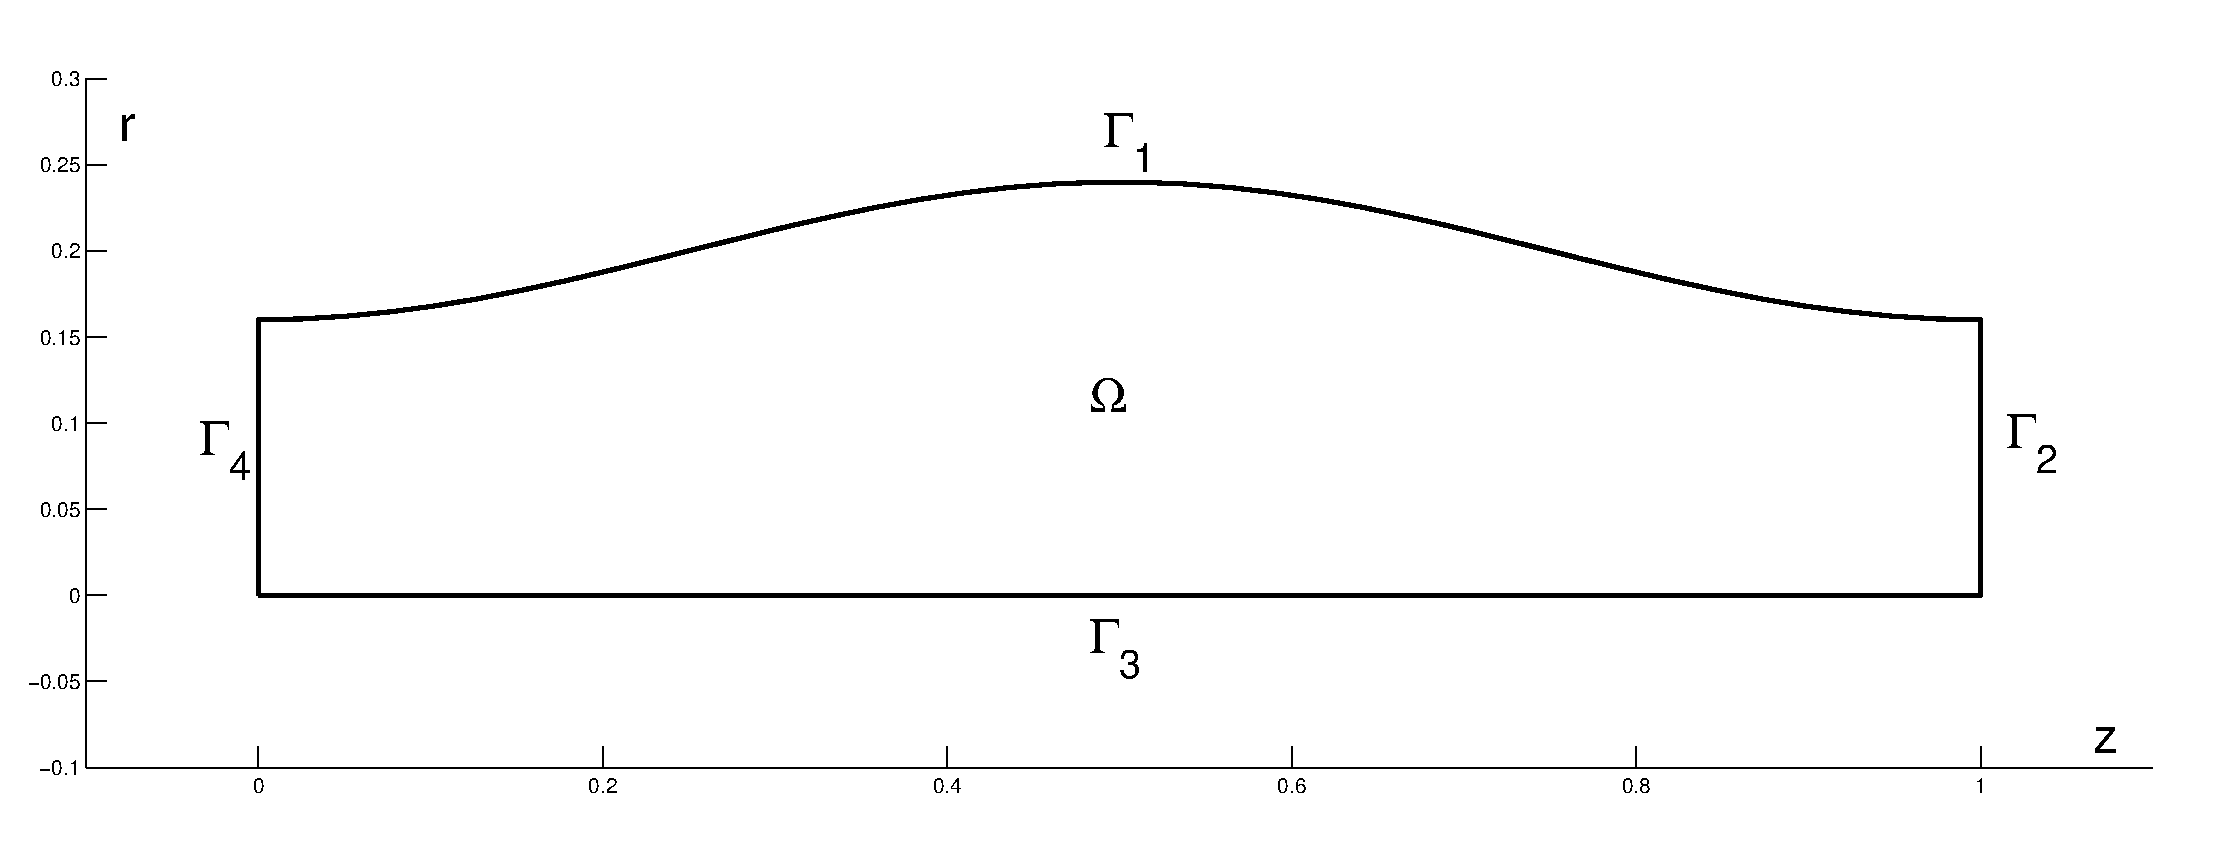
\includegraphics[scale=0.4]{images/mirror_matlab.eps}
\caption{Computational domain $\Omega$ for the fixed-boundary problem.}\label{fig:mirror_domain}
\end{figure}

From the physics of the problem, it makes sense to impose the following boundary conditions:
\begin{itemize}
  \item On $\Gamma_1$ Dirichlet;
  \item On $\Gamma_2$ periodicity with $\Gamma_4$
\end{itemize}
which are equivalent to
\begin{equation}\label{eq:bc}
  \begin{cases}
    \psi|_{\Gamma_1}=g(z)\\
    \psi|_{\Gamma_2}=\psi|_{\Gamma_4}\\
    \nabla\psi|_{\Gamma_2}=\nabla\psi|_{\Gamma_4}.
  \end{cases}
\end{equation}

It is important to notice that no condition are imposed on the boundary $\Gamma_3$. This happens since we are using the axisymmetric hypothesis therefore no condition can be imposed there. In the following section, cmp. Sec.(\ref{sec:weak_formulation}), this fact will come out naturally from the weak formulation.

Therefore the equilibrium problem is the following:
\begin{equation}\label{eq:equlibrium_and_bc}
  \begin{cases}
    -\Delta^*\psi+\mathbf{F}\cdot\nabla\psi-r^2\:f=0 & \mathrm{in}\:\Omega\\
    \psi(z,\gamma(z))=g(z)& \\
    \psi(0,r)=\psi(1,r)\\
    \nabla\psi(0,r)=\nabla\psi(1,r).
  \end{cases}
\end{equation}

\section{Weak formulation}\label{sec:weak_formulation}
For the numerical discretization we need to derive the weak form, or distributional formulation, of Eq.(\ref{eq:compact_equlibrium}), which requires less regularity on the solution, at the expense of increasing the regularity requirement on the test functions.
\medskip

The Laplace operator in cylindrical coordinates, under axisymmetric hypothesis, assumes the following expression
\begin{equation}\label{eq:laplace_operator}
  \Delta f=\frac{1}{r}\frac{\partial}{\partial r}\bigg(r\frac{\partial f}{\partial r}\bigg)+\frac{\partial^2f}{\partial z^2}=\frac{\partial^2f}{\partial r^2}+\frac{\partial^2f}{\partial z^2}+\frac{1}{r}\frac{\partial f}{\partial r},
\end{equation}
while the gradient has the same expression
\begin{equation}\label{eq:gradient_operator}
  \nabla f=\frac{\partial f}{\partial r}\mathbf{e}_r+\frac{\partial f}{\partial z}\mathbf{e}_z,
\end{equation}
therefore the Grad-Shafranov operator, cmp. Eq.(\ref{eq:GS_operator}), defined as
\begin{equation}
  \Delta^* \psi=\Delta\psi-\frac{2}{r}\partial_r\psi;
\end{equation}
assumes the following formulation
\begin{equation}\label{eq:GS_explicit}
  \Delta^* \psi=\partial_{rr}\psi+\partial_{zz}\psi-\frac{1}{r}\partial_r\psi.
\end{equation}
We can rewrite Eq.(\ref{eq:compact_equlibrium}), substituting inside Eq.(\ref{eq:GS_explicit}) and multiplying  everything by $r$ to get rid of the denominator, as
\begin{equation}\label{eq:compact_equlibrium_bis}
  -r\:(\partial_{rr}\psi+\partial_{zz}\psi)+\partial_r\psi+r\:\mathbf{F}\cdot\nabla\psi-r^3\:f=0
\end{equation}
which in ,distributional formulation, becomes
\begin{equation}\label{eq:compact_equlibrium_var}
  -\int_{\Omega}(\partial_{rr}\psi+\partial_{zz}\psi)\:rv\:\mathrm{d}\Omega + \int_{\Omega}\partial_r\psi\:v\:\mathrm{d}\Omega + \int_{\Omega}\mathbf{F}\cdot\nabla\psi\:rv\:\mathrm{d}\Omega - \int_{\Omega}r^3\:f\:v\:\mathrm{d}\Omega = 0.
\end{equation}
Applying the divergence theorem to the first term
\begin{equation}\label{eq:divergence_theorem}
  -\int_V (\partial_{rr}u+\partial_{zz}u)\:w\:\mathrm{d}V= \int_V \nabla u\cdot\nabla w\mathrm\:{d}V-\int_S w\nabla u\cdot\mathrm{d}\mathbf{S},
\end{equation}
taking $w=rv$ and $u=\psi$ over the domain $\Omega$, we obtain
\begin{equation}\label{eq:weak_GS_second_order_term}
  -\int_{\Omega}(\partial_{rr}u+\partial_{zz}u)\:rv\:\mathrm{d}\Omega=\int_\Omega \nabla\psi \cdot\nabla(rv)\:\mathrm{d}\Omega -\int_{\partial\Omega} rv\nabla \psi\cdot\mathrm{d}\mathbf{\partial\Omega}.
\end{equation}
The volume integral of Eq.(\ref{eq:weak_GS_second_order_term}), using the fact that
\begin{equation}
  \nabla(rv)=r\nabla v+v\left(\begin{array}{c}0\\1\end{array}\right),
\end{equation}
can be rewritten as
\begin{equation}
  \int_\Omega\nabla\psi \cdot\nabla(rv)\:\mathrm{d}\Omega=\int_\Omega r\:\nabla\psi \cdot\nabla v\:\mathrm{d}\Omega+\int_{\Omega}\partial_r\psi\:v\:\mathrm{d}\Omega
\end{equation}
while the surface integral becomes
\begin{equation}
  -\int_{\partial\Omega} rv\nabla \psi\cdot\mathrm{d}\mathbf{\partial\mathbf{\Omega}} = -\int_{\Gamma_1} rv\nabla \psi\cdot\mathrm{d}\mathbf{\Gamma}_1 - \int_0^{\gamma(1)}r(v\:\partial_z\psi)|_{z=1}\:\mathrm{d}r + \int_0^{\gamma(0)}r(v\:\partial_z\psi)|_{z=0}\:\mathrm{d}r
\end{equation}
where the line integral over $\Gamma_3$ is null due to the fact that $r=0$. Moreover it holds
\begin{equation}
  \begin{split}
    -\int_0^{\gamma(1)}r(v\:\partial_z\psi)|_{z=1}\:\mathrm{d}r + \int_0^{\gamma(0)}r(v\:\partial_z\psi)|_{z=0}\:\mathrm{d}r=\\
  =\int_0^{\gamma(1)=\gamma(0)}r\big((v\:\partial_z\psi)|_{z=0}-(v\:\partial_z\psi)|_{z=1}\big)\mathrm{d}r;
  \end{split}
\end{equation}
the quantity $(v\:\partial_z\psi)|_{z=0}-(v\:\partial_z\psi)|_{z=1}$ is the jump of the function $\partial_z\psi \:v$ on the line where we impose the periodicity, therefore $\Gamma_2\equiv\Gamma_4$. From the periodicity conditions, cmp. Eq.(\ref{eq:equlibrium_and_bc}), we know that $\psi\in C^1(\Gamma_2\equiv\Gamma_4)$ and $v\in C^0(\Gamma_2\equiv\Gamma_4)$ therefore $\partial_z\psi\:v\in C^0(\Gamma_2\equiv\Gamma_4)$ and its jump on that line must be equal to zero which leads to
\begin{equation}
  \int_0^{\gamma(1)=\gamma(0)}r\big((v\:\partial_z\psi)|_{z=0}-(v\:\partial_z\psi)|_{z=1}\big)\mathrm{d}r=0.
\end{equation}
Therefore we can rewrite Eq.(\ref{eq:weak_GS_second_order_term}) as
\begin{equation}
  -\int_{\Omega}(\partial_{rr}u+\partial_{zz}u)\:rv\:\mathrm{d}\Omega=\int_\Omega r\:\nabla\psi \cdot\nabla v\:\mathrm{d}\Omega+\int_{\Omega}\partial_r\psi\:v\:\mathrm{d}\Omega-\int_{\Gamma_1} rv\nabla \psi\cdot\mathrm{d}\mathbf{\Gamma}_1
\end{equation}
which leads to the the following weak formulation for Eq.(\ref{eq:equlibrium_and_bc})
\begin{equation}\label{eq:GS_BC_weak}
  \begin{split}
    \int_\Omega r\:\nabla\psi \cdot\nabla v\:\mathrm{d}\Omega+2\int_\Omega v\:\partial_r \psi\:\mathrm{d}\Omega+\int_\Omega rv\:\mathbf{F}(\psi,B)\cdot\nabla\psi\:\mathrm{d}\Omega +\\ -\int_\Omega r^3vf\:\mathrm{d}\Omega =\int_{\Gamma_1} rv\nabla \psi\cdot\mathrm{d}\mathbf{\Gamma}_1\quad\forall v\in V.
  \end{split}
\end{equation}
\medskip

In order to define the space of solution and test functions, the integrals in Eq.(\ref{eq:GS_BC_weak}) must have sense, which means that integrands must be in $L^1(\Omega)$. To satisfy this condition we use the H\"{o}lder's inequality in his generalized version: assume that $p\in(0, \infty)$ and $p_1,\dots, p_n  \in (0, \infty]$ such that
\begin{equation}
  \sum_{k=1}^n \frac1{p_k}=\frac{1}{p}
\end{equation}
than
\begin{equation}
  f_k\in L^{p_k}(\mu)\;\;\forall k\in\{1,\ldots,n\}\implies\prod_{k=1}^n f_k \in L^p(\mu).
\end{equation}
Since $r\in L^\infty(0,R)$ and also its positive integer powers, then we required at least that $\nabla \psi$, $\psi$ and $\nabla v$, $v$ are in $L^2(\Omega)$,
i.e.$\psi,v\in H^1(\Omega)$. In addition we need the nonlinear terms be $\mathbf{F}\in L^\infty(\Omega)$ and $f\in L^2(\Omega)$. These last assumptions are not trivial.
\medskip

We want to use a Galerkin formulation therefore we need to define the test space and the trial space as close as possible. Usually the space where we look for the solution is influenced by the Dirichlet conditions, in particular that ones in (\ref{eq:bc}) can be included fully in the trial space, instead the test functions can vanish on the Dirichlet boundary. Let the test space be
\begin{equation}\label{eq:test_space}
\begin{split}
 V&=\{v\in H^1(\Omega):\:v|_{\Gamma_1}=0\}\cap\{v\in H^1(\Omega):\:v|_{\Gamma_3}=0 \}\\
&\cap\{v\in C^0(\overline{\Omega}):v|_{\Gamma_2}=v|_{\Gamma_4}\}=V_0^{\Gamma_1}\cap V_0^{\Gamma_3} \cap C^0(\Omega)=V_0 \cap C^0(\Omega)
\end{split}
\end{equation}
and let the trial space be
\begin{equation}\label{eq:trial_space}
 W=V_0^{\Gamma_3}\cap\{v\in H^1(\Omega):\:v|_{\Gamma_1}=g \}\cap C^0_{p_z}(\Omega)=V_0^{\Gamma_3}\cap V_g^{\Gamma_1}\cap C^0(\Omega).
\end{equation}

$V_g$ is an affine manifold of $H^1(\Omega)$, not a subspace of $H^1(\Omega)$ therefore it is not possible to express the solution as an expansion of a basis as it is not true that linear combinations of elements in $V_g$ are still elements of $V_g$. There are two usual ways to treat this problem:
\begin{itemize}
  \item if $g\in H^{1/2}(\Gamma_1)$, so $\exists\: R_g\in H^1(\Omega)$, called Dirichlet lift, such that $R_g|_{\Gamma_1}=g$, the solution can be split into two contributions $\psi=\psi_0+R_g$, where $\psi_0\in V$ and $R_g\in V_g$;
  \item the matrix system can be assembled including all degrees of freedom of our approximation and then we can zeroing the rows which correspond to the Dirichlet degree of freedom,
  placing a unit term on the diagonal and setting the right-hand side to the known values. It means that we look for $\psi\in V_0^{\Gamma_3}\cap C^0(\Omega)$ such that $\psi|_{\Gamma_1}=g$.
\end{itemize}
Numeric approximation makes easy the task of building the Dirichlet lift: it can be done from an approximation of the boundary data $g$, generally as a linear combination of the basis function on the Dirichlet boundaries. This splitting technique is useless when we have to treat nonlinear term and we can only apply the zeroing technique at the final system. So we look for the complete solution though the knowledge of the value of the solution on the Dirichlet boundaries making its calculations useless and the final problem will not be yet symmetric since we request, in principle, different constraints to the trial and test spaces.

In the light of space definitions, the weak formulation (\ref{eq:GS_BC_weak}) becomes
\begin{equation}\label{eq:prob_var}
  \left\{\begin{array}{ll}\textrm{Find $\psi\in W$ such that}\\
  \textrm{$a(\psi,v)=0$ $\forall v\in V$ and $\psi|_{\Gamma_3}=g$}\\
\end{array}\right.
\end{equation}
where $a(\psi,v)$ is the nonlinear map $a:W_g\times V_0\rightarrow\mathbb{R}$:
\begin{equation}\label{eq:a_operator}
  a(\psi,v)=\int_\Omega \big(r\:\nabla\psi \cdot\nabla v+2v\:\partial_r \psi+rv\:\mathbf{F}\cdot\nabla\psi -r^3vf\big)\mathrm{d}\Omega.
\end{equation}
Since the mapping is nonlinear $a(u_0+R_g,v)\neq a(u_0,v)+a(R_g,v)$ which implies that it is not possible to use the Dirichlet lift to impose Dirichlet boundary conditions but it is necessary to apply the zeroing technique.

\section{Spectral element method}\label{sec:spectral_aproximation}
Spectral Element Method (SEM) is a particular type of Finite Element Method (FEM). The difference with a classical FEM are the interpolation nodes, indeed for the former they are distributed at position corresponding to the zeros of a family of orthogonal polynomials while for the latter on some special points on the element.

The choice of an orthogonal basis allows the accuracy of the method to be spectral, i.e. the rate of convergence of the interpolation with respect to degree $p=\min p_m$ of polynomial is faster than any power of $1/p$. Indeed its order of convergence is related to the maximum regularity of the solution, namely it is exponential for a very smooth solution but this fast convergence is easily lost if the solution has finite regularity or if the domain is irregular. In this case the order of convergence is reduced to a classical FEM where it is fixed by the choice of the basis and it does not depend on the regularity of the solution.

Unfortunately the stiffness matrix which arise from a SEM discretization is more dense than the one generated by a classical FEM, therefore the computational cost is higher. For this reason it is worthing to use this type of discretization when a smooth solution is expected, which it is our case since we are solving an equilibrium problem.

In the following we give a brief overview of the method and we point out the concepts which will be important in the implementation of the code. For an introductory description cmp. \cite{QUARTERONI} while for a more advance analysis  of the method cmp. \cite{CHQZ06} for 1-D domains and \cite{CHQZ07} for multidimensional domains. For what concern the implementation cmp. \cite{KARNIADAKIS} and \cite{HENDERSON}.

\subsection{Spectral element}\label{subsec:sem_element}
The mirror domain $\Omega\subset\mathbb{R}^2$, see Fig.(\ref{fig:mirror_domain}), can be represented as a union of $M$ disjoint quadrilateral sub-domain $\Omega_m$ with straight edges:
\begin{equation}
  \Omega\approx\mathcal{T}_h=\bigcup_{m=1}^M\Omega_m.
\end{equation}
We consider only a geometrically conforming partition which means that neighboring sub-domains share either a vertex or a complete edge. Let $h$ be
\begin{equation}
  h=\max_m h_m=\max_m\big(\mathrm{diam}(\Omega_m)\big)
\end{equation}
where $\mathrm{diam}(\Omega_m)$ is the length of longest edge of the element $\Omega_m$. Moreover we assume that these diameters are uniformly bounded below.

We define \textit{spectral element} the triplet $(\Omega_m, \mathbb{Q}_{p_m}(\Omega_m),\{v_k\})$ where
\begin{itemize}
  \item $\Omega_m$ convex quadrilateral $\subset \Omega$ so that $\Omega_m=\textbf{F}_m(\hat{\Omega})$;
  \item $\mathbb{Q}_{p_m}(\Omega_m)$ space of polynomials of degree $\leq p_m$ in each coordinate in $\Omega_m$, which dimension is $N=(p_m+1)^2$
  \item $\{v_k\}_0^N$ degrees of freedom for $\mathbb{Q}_{p_m}(\Omega_m)$
\end{itemize}

To standardize the local basis on $\Omega_m$, we introduce a logical domain $\hat{\Omega}=[-1,1]\times[-1,1]$ and an invertible bilinear map $\textbf{F}_m$,
\begin{equation}
\textbf{F}_m:\hat{\Omega} \rightarrow \Omega_m,
\end{equation}
between these two spaces. The maps which we will use it is not affine therefore it does not preserve the parallel property of edges and faces therefore the partition of the domain, in general, is not made by parallelogram. The explicit equation of the map used is given in Sec.(\ref{subsec:mapping}).
\medskip

We want to approximate our problem projecting it onto a space of functions that are piecewise polynomials on the element $\Omega_m$. We define the family of finite spaces of trial functions $W_\delta\subset W\subset C^0(\Omega)$
\begin{equation}
  W_\delta=\{w\in W:\: w|_{\Omega_m}=\hat{v}\circ \mathbf{F}^{-1}_m,\:\hat{v}\in\mathbb{Q}_{p_m}(\hat{\Omega})\:\forall\Omega_m\in\mathcal{T}_h\}
\end{equation}
and, analogously, the finite trial space is
\begin{equation}
 V_\delta=\{v\in V:\: v|_{\Omega_m}=\hat{v}\circ \mathbf{F}^{-1}_m,\:\hat{v}\in\mathbb{Q}_{p_m}(\hat{\Omega})\:\forall\Omega_m\in\mathcal{T}_h\}.
\end{equation}
where the subindex $\delta$ is an abridged notation for \textquotedblleft{discrete\textquotedblright} that accounts for the geometric sizes $h$ and the polynomial degrees $p=\min_m(p_m)$.

Ergo these two spaces are formed by functions that are images of polynomial functions $\hat{v}\in\mathbb{Q}_{p_m}(\Omega_m)$ through $\mathbf{F}_m$, so $v(x,y)=\hat{v}(\mathbf{F}_m^{-1}(x,y))$ $\forall(x,y)\in\Omega_m$. It is important to notice that $\mathbf{F}_m$ describes only the geometric transformation, whereas the function $v$ is not more a polynomial of the same degree of $\hat{v}$ as $\mathbf{F}_m$ is not affine.

In general both the mapping $\mathbf{F}_m$ and the polynomial order $p_m$  can vary within each element $\Omega_m$ thereby permitting both $h$- type refinement which alters $\mathbf{F}_m$ and $M$, and $p$-type refinement witch alters $p_m$. It is for this reason that SEM is called also $hp$-FEM. The polynomial basis chosen is given in Sec.(\ref{sec:modal_basis}).

\subsection{SEM}
The \textit{Galerkin approximation} consists in substitute the exact solution $\psi$ with the approximate solution $\psi_{\delta}$ into the weak formulation of our problem, cmp. Eq.(\ref{eq:prob_var}),
\begin{equation}
 \psi_\delta\in W_\delta:\: a(\psi_\delta,v_\delta)=0\quad\forall v_\delta\in V_\delta
\end{equation}
or, exploiting the linearity of the integral operator $a_m(u,v)=a(u,v)|_{\Omega_m}$,
\begin{equation}\label{eq:sem_formulation}
 \psi_\delta\in W_\delta:\: \sum_{m=1}^M a_m(\psi_\delta,v_\delta)=0\quad\forall v_\delta\in V_\delta
\end{equation}
which is the SEM formulation of our original problem.
\medskip

The discrete solution $\psi_{\delta}$ can be written as the truncated series on the global basis $\{\phi_k\}\in W_{\delta}$ or in the local one $\{\phi_j^{(m)}\}\in\mathbb{Q}_{p_m}(\Omega_m)$ in the following way
\begin{equation}\label{eq:solution_series}
  \psi_\delta=\sum_k \psi_k \phi_k=\sum_{m=1}^{M} \sum_{j=0}^{p^2_m} \psi^{(m)}_j \phi_j^{(m)}.
\end{equation}
Taking the scalar product of Eq.(\ref{eq:solution_series}) with $\phi_i$
\begin{equation}
  (\psi_\delta,\phi_i)=\sum_k \psi_k (\phi_k,\phi_i)
\end{equation}
we obtain the definition of the coefficients of the expansion
\begin{equation}\label{eq:expansion_coeff}
 \psi_k=\sum_l M^{-1}_{kl}(\psi_\delta,\phi_l)
\end{equation}
where $M^{-1}$ is the inverse matrix of mass matrix $M_{ik}=(\phi_k,\phi_i)$.
\medskip

Substituting Eq.(\ref{eq:solution_series}) in Eq.(\ref{eq:sem_formulation}), using the Einstein convention, the local problem becomes a non linear algebraic problem:
\begin{equation}\label{eq:algebraic_system}
  \left\{\begin{array}{ll}\textrm{Find $\{\psi^{(m)}_j\}$ such that}\\
  \textrm{$A^{(m)}_{ij} \psi_j^{(m)}=0,\:\forall i\in\{0,\dots,p^2_m\}$}\\
\end{array}\right.
\end{equation}
where $A$ is the local stiffness matrix.

The global stiffness matrix is formed assembling all the local one \textquotedblleft{gluing\textquotedblright} together the local basis to obtain a global $C^0$ basis, cmp. Sec.(\ref{sec:global_assembling}).

\subsection{SEM-NI}
Now we want do derive the final discrete formulation that we are going to implement and solve. Since all the functions will be mapped in the logical domain through the mapping $\mathbf{F}_m$, cmp. Sec.(\ref{subsec:sem_element}), we rewrite how the quantities involved are transformed trough this mapping. For what concern the integral, it holds the following identity
\begin{equation}\label{eq:integral_transf}
  \int_{\Omega_m} f(z,r)\:\mathrm{d}\mathbf{x} =\int_{\hat{\Omega}}f(\mathbf{F}_m(\hat{x},\hat{y}))|\det(J_{\mathbf{F}_m}(\hat{x},\hat{y}))|\:\mathrm{d}\hat{\mathbf{x}}
\end{equation}
where $J_{\mathbf{F}_m}$ is the jacobian of our mapping. Moreover, using the chain rule, it is possible to find that the gradient of a function is transformed as
\begin{equation}\label{eq:grad_transf}
  \nabla f(x,y)=J_{\mathbf{F}_m}^{-T}(\hat{x},\hat{y})\hat{\nabla}\hat{f}(\hat{x},\hat{y})
\end{equation}
where $\hat{f}=f\circ\mathbf{F}_m$ and $\hat{\nabla}(\cdot)=\left(\begin{array}{c}\partial_{\hat{x}}(\cdot)\\\partial_{\hat{y}}(\cdot)\end{array}\right)$.
\medskip

Instead of evaluating the exact integrals to find the contributes of the stiffness matrix, we substitute the inner product with the discrete version using a quadrature formula:
\begin{equation}\label{eq:quadrature_formula}
  \int_{\Omega_m} f(z,r)\:\mathrm{d}\mathbf{x} \approx\sum_{n=0}^{N}w_n f(z_n,r_n).
\end{equation}
The couples $(z_n,r_n)$ are the quadrature nodes while $w_n$ are the weights with $n\in\{0,\dots,N\}$. If we apply Eq.(\ref{eq:integral_transf}) to the quadrature formula (\ref{eq:quadrature_formula}) we obtain the quadrature formula in the logical domain
\begin{equation}
  \begin{split}
    \int_{\Omega_m} f(z,r)\:\mathrm{d}\mathbf{x} =\int_{\hat{\Omega}}f(\mathbf{F}_m(\hat{x},\hat{y}))|\det(J_{\mathbf{F}_m}(\hat{x},\hat{y}))|\:\mathrm{d}\hat{\mathbf{x}}\approx&\\
    \approx\sum_{n=0}^{N}w_k \hat{f}(\hat{x}_n,\hat{y}_n)|\det(J_{\mathbf{F}_m}(\hat{x}_n,\hat{y}_n))|.\\
  \end{split}
\end{equation}
Therefore the nodes are defined on the logical domain; more precisely both the node and the weights are obtained with a tensor product of the nodes and the weights of the quadrature formula
on one-dimensional interval [-1,1]. For the expression of the nodes and weigths used cmp. Sec.(\ref{sec:gaussian_integration}).

If we substitute the local integrals with their discrete approximations we obtain the following SEM-NI, where NI states for Numerical Integration, version of (\ref{eq:sem_formulation})
\begin{equation}\label{eq:SEM_NI}
  \psi^*_\delta\in W_\delta:\: \sum_{m=1}^M a_m^{N_m}(\psi^*_\delta,v_\delta)=0\quad\forall v_\delta\in V_\delta
\end{equation}
where $N_m+1$ is the number of quadrature nodes used.
\medskip

Now we can rewrite our variational system, cmp. Eq.(\ref{eq:prob_var}), in the discrete formulation. Firstly we need to rewrite Eq.(\ref{eq:a_operator}) in the logical domain. Using Eq.(\ref{eq:integral_transf}) and Eq.(\ref{eq:grad_transf}) we can rewrite the first term as
\begin{equation}\label{eq:first_logical}
  \begin{split}
    \int_{\Omega_m}r\:\nabla\psi\cdot\nabla v\:\mathrm{d}\Omega_m &=\int_{\hat{\Omega}} \mathbf{F}^r_m(J_{\mathbf{F}_m}^{-T}\:\hat{\nabla}\hat{\psi})^T\:
    J_{\mathbf{F}_m}^{-T}\:\hat{\nabla}\hat{v}\:|\det(J_{\mathbf{F}_m})|\:\mathrm{d}\hat{\Omega}=\\
    &=\int_{\hat{\Omega}} \hat{\nabla}^T\hat{\psi}\:J_{\mathbf{F}_m}^{-1}\:J_{\mathbf{F}_m}^{-T}\:\hat{\nabla}\hat{v}\:|\det(J_{\mathbf{F}_m})|\:\mathrm{d}\hat{\Omega},\qquad\forall\Omega_m\in\mathcal{T}_h
  \end{split}
\end{equation}
where with $\mathbf{F}_m^r$ we indicate the second component of the image of the transformation $\mathbf{F}_m$.

Similarly, for the second term we have
\begin{equation}\label{eq:second_logical}
  \begin{split}
    &\int_{\Omega_m}2\:v\:\partial_r\psi\:\mathrm{d}\Omega_m =\int_{\Omega_m}2v\:((0,1)\cdot\nabla\psi)\:\mathrm{d}\Omega_m=\\
    &=\int_{\hat{\Omega}}2\hat{v}\:((0,1)\cdot(J_{\mathbf{F}_m}^{-T}\:\hat{\nabla}\hat{\psi})\:|\det(J_{\mathbf{F}_m})|\:\mathrm{d}\hat{\Omega}=\\
    &=\int_{\hat{\Omega}}2\hat{v}\:(\partial_{\hat{x}}\hat{\psi}\:\partial_r\hat{x}+\partial_{\hat{y}}\hat{\psi}\:\partial_r\hat{y})\:|\det(J_{\mathbf{F}_m})|\:\mathrm{d}\hat{\Omega},\qquad\forall\Omega_m\in\mathcal{T}_h,
  \end{split}
\end{equation}
while for the third one we obtain
\begin{equation}\label{eq:third_logical}
  \int_{\Omega_m}rv\:\mathbf{F}\cdot\nabla\psi\:\mathrm{d}\Omega_m = \int_{\hat{\Omega}}\mathbf{F}_m^r\hat{v}\:\mathbf{\hat{F}}\:J_{\mathbf{F}_m}^{-T}\:\:\hat{\nabla}\hat{\psi}\:|\det(J_{\mathbf{F}_m})|\:\mathrm{d}\hat{\Omega},\qquad\forall\Omega_m\in\mathcal{T}_h,
\end{equation}
and for the last one we find
\begin{equation}\label{eq:fourth_logical}
  -\int_{\Omega_m}r^3v\:f\:\mathrm{d}\Omega_m = -\int_{\hat{\Omega}}(\mathbf{F}_m^r)^3\hat{v}\:\hat{f}\:|\det(J_{\mathbf{F}_m})|\:\mathrm{d}\hat{\Omega},\qquad\forall\Omega_m\in\mathcal{T}_h.
\end{equation}
We want to point out that $\mathbf{F}$ and $\mathbf{F}_m$ are two unrelated quantities: indeed the former is the functional which represent the first order term of the equation, cmp. Eq.(\ref{eq:functional_F}), while the latter is the mapping from the logical domain to the physical one.
\medskip

We can finally obtain the explicit formulation of our SEM-NI problem, cmp. Eq.(\ref{eq:SEM_NI}), summing the four terms just obtained, cmp. Eq.(\ref{eq:first_logical}), Eq.(\ref{eq:second_logical}), Eq.(\ref{eq:third_logical}) and Eq.(\ref{eq:fourth_logical}), substituting the exact integral with the quadrature formula, cmp. Eq.(\ref{eq:quadrature_formula}), choosing the test function $v_{\delta}$ among the basis function $\phi_i\in V_{\delta}$ and approximating the exact solution $\psi$ in series, cmp. Eq.(\ref{eq:solution_series}). This procedure leads, for what concern the degrees of freedom, to the following discrete formulation
\begin{equation}\label{eq:discrete_formulation}
  \begin{split}
    &\sum_m \bigg\{\sum_j \psi_j \sum_n w_n\:\mathbf{F}_m^r(\mathbf{\hat{x}}_n)\hat{\nabla}\hat{\phi}_j(\mathbf{\hat{x}}_n)J_{\mathbf{F}_m}^{-1}(\mathbf{\hat{x}}_n)J_{\mathbf{F}_m}^{-T}(\mathbf{\hat{x}}_n)\hat{\nabla}\hat{\phi}_i(\mathbf{\hat{x}}_n)|\det(J_{\mathbf{F}_m}(\mathbf{\hat{x}}_n))| +\\
    &+2\:\sum_j\psi_j\sum_n w_n[\frac{\partial\hat{x}}{\partial r},\frac{\partial\hat{y}}{\partial r}]_{\big|_{\mathbf{\hat{x}}_n}}\hat{\nabla} \hat{\phi}_j(\mathbf{\hat{x}}_n)\:\hat{\phi}_i(\mathbf{\hat{x}}_n)|\det(J_{\mathbf{F}_m}(\mathbf{\hat{x}}_n))|+\\
    &+\sum_j \psi_j \sum_n w_n\:\mathbf{F}_m^r(\mathbf{\hat{x}}_n)\mathbf{\hat{F}}(\sum_l\psi_l\hat{\phi}_l(\mathbf{\hat{x}}_n),\mathbf{\hat{x}}_n)J_{\mathbf{F}_m}^{-T}(\mathbf{x}_n)\hat{\nabla} \hat{\phi}_j(\mathbf{\hat x}_n)\hat{\phi}_i(\mathbf{\hat{x}}_n)|\det(J_{\mathbf{F}_m}(\mathbf{\hat{x}}_n))|+\\
    &-\sum_n w_n\:\mathbf{F}_m^r(\mathbf{\hat{x}}_n)^3 \hat{f}(\sum_l\psi_l\hat{\phi}_l(\mathbf{\hat{x}}_n),\mathbf{\hat{x}}_n)\hat{\phi}_i(\mathbf{\hat{x}}_n)|\det(J_{\mathbf{F}_m}(\mathbf{\hat{x}}_n))|\bigg\}=0, \qquad\forall i\in\mathcal{I}
  \end{split}
\end{equation}
where
\begin{equation}
\mathcal{I}=\sum_{m=1}^M\mathcal{I}_m
\end{equation}
and $\mathcal{I}_m$ is the number of local degrees of freedom. Instead, the summations over $j$ range in $\{0,\dots,\mathcal{I}_m+\mathcal{D}_m\}$ where $\mathcal{D}_m$ is the number of local non degrees of freedom due to the Dirichlet conditions. This is true since our discrete solution can be decomposed in the following way
\begin{equation}
  \psi^*_\delta=\sum_{k=0}^{\mathcal{I}+\mathcal{D}}\psi_k\phi_k=\sum_{m=1}^M \sum_{j=0}^{\mathcal{I}_m}\psi_j\phi_j+\sum_{m=1}^M \sum_{j=0}^{\mathcal{D}_m}\psi_j\phi_j
\end{equation}
and
\begin{equation}
  \{\psi_j\}_{\mathcal{D}}=\{g_j\}_{\mathcal{D}}
\end{equation}
where $g_j$ are the coefficients of the projection of the boundary condition which can be find solving the system (\ref{eq:expansion_coeff}) using $\psi_{\delta}=g$.

Finally we like to point out that in Eq.(\ref{eq:discrete_formulation}) the trial space and test space coincide. Indeed we are taking the trial space without imposing the Dirichlet condition therefore they are exactly the same space, cmp Eq.(\ref{eq:trial_space}) and Eq.(\ref{eq:test_space}). The Dirichlet boundary condition are imposed later using the zeroing technique.
\medskip

For what concern the approximation error, it is possible to demonstrate, that the following inequality holds
\begin{equation}
  \|u-u_\delta\|_{H^m}\leq C(s)\: h^{\min(p+1,s)-m}\:p^{m-s}\|u\|_{H^s}.
\end{equation}

\subsection{The Abstract Newton method}\label{subsec:newton_method}
The discrete formulation obtained, cmp. Eq.(\ref{eq:discrete_formulation}), in general gives origin to a non linear algebraic system when $f$ or $\mathbf{F}$ are function of the solution $\psi$. A common way to deal with this is to use the Abstract Newton Method which consist to linearize the system using the functional derivative.
\medskip

Let $V$  be a Sobolev space, and let $F$ be a non linear operator s.t. $F\,:\,V\rightarrow V$. We consider the problem
\begin{equation}
  \left\{\begin{array}{ll}
    \textrm{Find $u^{\star}\in V$ such that}\\
    \textrm{$F(u^{\star})=0.$}\\
  \end{array}\right.
\end{equation}
The Abstract Newton method, given an initial guess $u^{0}\in V$, proceeds in this way:
\begin{enumerate}
\item Calculation of the increment $\delta u^{(k)}$ s.t.
\begin{equation}
  \mathcal{F}(u^{(k)})\delta u^{(k)}=-F(u^{(k)})
\end{equation}
where $\mathcal{F}\,:\,V\rightarrow\mathcal{L}(V;V)$ is the Gateux derivative, cmp. \cite{SERRA}, related to $F$.
\item Updating of the solution
\begin{equation}
  u^{(k+1)}=u^{(k)}+\delta u^{(k)}.
\end{equation}
\end{enumerate}
This steps are repeated until the following convergence criterion is satisfied
\begin{equation}
\| u^{(k+1)}-u^{(k)}\|_{L^{\infty}(\Omega)}\leq\varepsilon
\end{equation}
where $\varepsilon$ is a given tolerance. The Gateux derivative is defined as
\begin{equation}
  \mathcal{F}(u)\delta u=\lim_{h\rightarrow0}\frac{F(u+h\delta u)-F(u)}{h}.
\end{equation}

It has been proved that: if $F$ is Lipschitz continuous in $V_{\varepsilon}^{\star}=\{v\in V\:\textrm{s.t.}\:\| u^{\star}-v \|_{V}\:\leq\varepsilon\}$, where $\varepsilon$ is suitably fixed, then $\exists\:\varepsilon'\in(0,\varepsilon]$ s.t. $\forall u^{(0)}\in V_{\varepsilon'}^{\star}$ the  sequence $\{ u^{(k)}\}$ converges in mean square to $u^{\star}$. Therefore this theorem guarantees the local convergence of the method but it depends on how close is the initial solution to the exact solution.

For this reason the updating of the solution can be modified in the following way
\begin{equation}
  u^{(k+1)}=u^{(k)}+\tau_{k}\,\delta u^{(k)}
\end{equation}
where $\tau_{k}$ is the damping coefficient. The latter is initially equal to one but if $\| F(u^{(k+1)})\|_{L^{\infty}(\Omega)}\leq\| F(u^{(k)})\|_{L^{\infty}(\Omega)}$ we proceed with the next Newton's iteration, otherwise, $\tau_{k}$ becomes $\frac{\tau_{k}}{2}$ and $u^{(k+1)}$ is recalculated until $\| F(u^{(k+1)})\|_{L^{\infty}(\Omega)}>\|F(u^{(k)})\|_{L^{\infty}(\Omega)}$.
\medskip

In our case the operator which we want to linearize is $a(\psi,v)$, cmp. Eq.(\ref{eq:a_operator}), therefore, in the light of the Newton method introduced, we have $F(\psi)=a(\psi,v)$ and $V$ is the usual test space, cmp. Eq.(\ref{eq:test_space}). To be precise, $V$ should be the trial space $W$, cmp. Eq.(\ref{eq:trial_space}), but since we are solving only the degrees of freedom and after we impose the Dirichlet boundary condition, we can simply use the test space.

The Gateux derivative $\mathcal{F}$ depends on $\mathbf{F}$ and $f$ therefore there will be evaluated case by case in Ch.(\ref{ch:numerical_results}) after the two functionals are been chosen to perform the different numerical simulations. With the same procedure used in the previous section, it is possible to find the discrete formulation of the derivative. It is also possible to evaluate the derivatives using some numerical approximation, usually finite difference, instead of evaluates them analytically but we choose to evaluate them in a precise way.
\medskip

An equivalent approach would be to evaluate the derivative $\mathcal{F}$ of the discretized form of our problem, cmp. Eq.(\ref{eq:discrete_formulation}), instead of discretized the derivative obtained from the exact functional.


\chapter{Mesh}\label{chapter:mesh}
In this chapter the part of the code regarding the management of a grid will be explained . The code can take as input all the information about the grid stored in a \verb|GMSH| file format and distributes all the grid information among N processes in an optimal way using the \verb|ParMETIS| and \verb|METIS| libraries. Both this part of the code and the chapter regarding it have been developed by a collaboration among Marco Agnese, Francesco Boffa and Marco Chiaramello. We decided to develop this parts together because each of us solves a problem on unstructured and conformal grids. Definitions of these grids will be explained in Sec.(\ref{subsection:gmsh}). In Fig.(\ref{fig:mesh_diagram}) it is possible to see the general structure of the code and the inheritances of the classes involved.

\begin{figure}
\centering
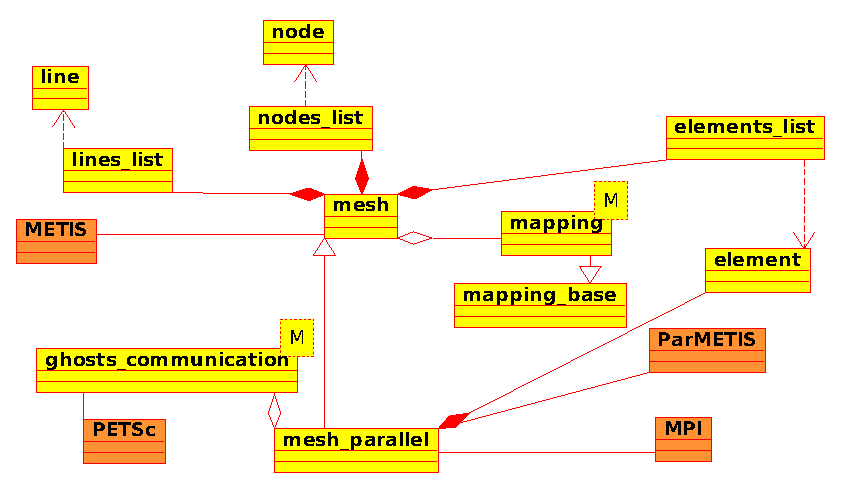
\includegraphics[scale=1]{images/mesh_diagram.eps}
\caption{Mesh management: classes structure.}
\label{fig:mesh_diagram}
\end{figure}

\section{Sequential mesh management}\label{section:mono_cpu}
The mesh management part of the code is structured in two main different classes. The class \verb|mesh| is implemented in a sequential way: its methods can be invocate in the same way when the code is run in a sequential or parallel way. Depending on which way it is run, its members will contain information of the global mesh or the local one.

The second class is \verb|mesh_parallel| and it manages the parallel methods, cmp. Sec.(\ref{section:multi_CPUs}).

\subsection{Data structures}\label{subsection:data_structures}
This part of the code involves the definition of some data structures in which all the information about the grid are stored.

\subsubsection{Nodes data structures}
The class \verb|node| contains all the methods to manage the information about the nodes of the grid. The physical coordinates are stored in a vector of \verb|double|, while the global index is stored an integer variable. A vector of classes \verb|node| is created in the class \verb|nodes_list|. The class \verb|nodes_list| contains also the methods to set the coordinates and the index of each node in the nodes list and to add an element to the vector of \verb|node|.

\subsubsection{Elements data structures}
In the class \verb|element| we have implemented all the methods necessary to completely define each element of the mesh. In particular, we have defined seven members of this class: four vectors of integers containing respectively the index of the vertex, the neighboring elements, the position of the corner elements and the relative position of the reference element on each neighboring element, and other two variables storing the global index of the element and the surface tag. The latter allows to define many different surfaces on the same domain, distinguishing the different portion. In the last variable (type: \verb|boolean|) is stored a flag which reveals if an element is a ghost or not, when the code is run in parallel. The vector of neighboring is set of variable dimension, due to the fact on a unstructured grid the number of elements neighboring a reference element is not fixed; both the elements situated on the sides and on the corner of the reference element are stored in this vector, cmp. Fig.(\ref{fig:element_neigh}) and Fig.(\ref{fig:element_corner}). The vector of position of the corner elements allows to determine, when the vector of neighboring has been created, on which corner each neighbor sharing one vertex with the reference element is located. The vector storing the relative position of the reference element on each neighboring element (called \verb|neighbor_cor_pos|) allows to reconstruct uniquely the position of each element respect to the others, regardless the orientation of each element. In the class \verb|element_list| a vector of \verb|element| is created, together with all the methods necessary to set the \verb|element| members. In the \verb|element_list| member variable called \verb|number_ghosts| is stored the number of ghosts allocated on each process, cmp. Sec.(\ref{section:multi_CPUs}).

\begin{figure}
\centering
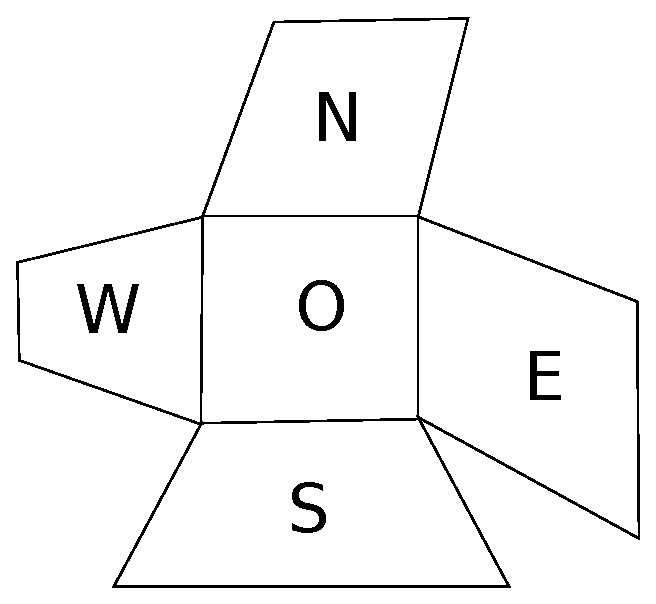
\includegraphics[scale=.45]{images/mono_cpu_data_structures_element_neigh}
\caption{Elements S,W,N,E are neighbors of element 0 located on its sides.}
\label{fig:element_neigh}
\end{figure}

\begin{figure}
\centering
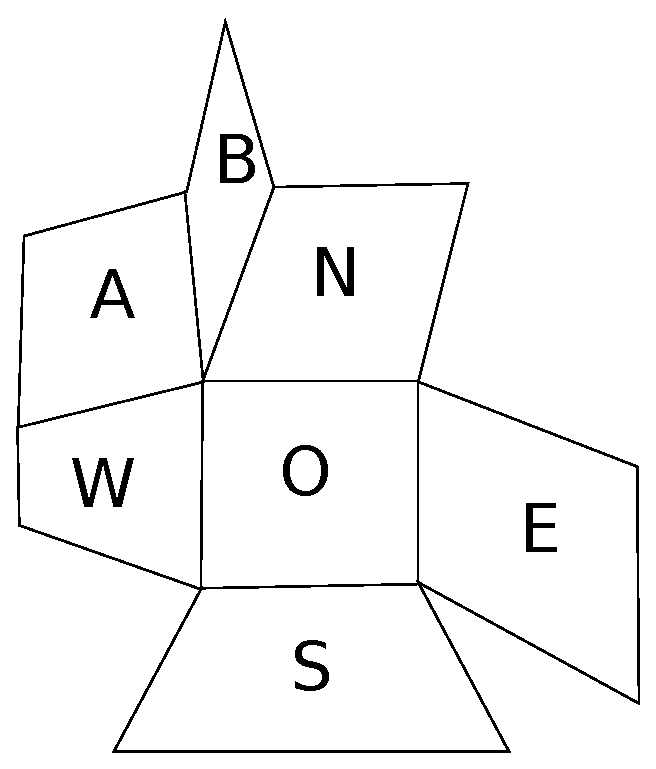
\includegraphics[scale=.45]{images/mono_cpu_data_structures_element_corner}
\caption{Elements A,B are neighbors of element 0 located on its corners.}
\label{fig:element_corner}
\end{figure}

\subsubsection{Lines data structures}
The class \verb|line| contains the methods to characterize the lines belonging to the border of the domain. In a vector of integers we store the vertexes of each line. In other four members of type \verb|int| we store the global index of the line, a tag, the index of the element to which the line belongs and the index of the side of the element in which the line is located, respectively. The tag indicates the type of boundary condition is imposed on that line. Then in the class \verb|lines_list| we create a vector of \verb|line|, together with all the methods necessary to set all the members of \verb|line|.

\subsection{Main methods involved}\label{subsection:mono_cpu_methods}
All the most important algorithms involved in the definition of the topology of the mesh are included in the class \verb|mesh|. In particular, the methods implemented in this class allows the user to read the grid information from a file (in a \verb|.msh| format ), to evaluate all the neighbors situated on each side of the reference element, to determine the elements situated on the corners, to define if an element is a border one. All these methods are reported in detail below.

\subsubsection{read\_file}
It takes as input the name of the file in which the grid information are stored. Following the \verb|GMSH| format (cmp. \ref{subsection:gmsh}), it stores the data in the classes (\verb|nodeslist|, \verb|elementslist| and \verb|lineslist|) converting from a string format to a numerical one.

\subsubsection{eval\_topology}
It reconstructs the topology of each element. This means that determines all the elements that share one or two vertexes with a reference element. This evaluation has been implemented using the command \verb|METIS_MeshToDual| of the \verb|Metis| library. All the neighboring elements are stored without making any difference if they are located on a side of the reference element or if they share a single vertex.
\medskip

For example, the vector of neighbors of the element 0 reported in Fig.(\ref{fig:mono_cpu__main_methods_involved__eval_topology}) will be:
\medskip

neighbors=[1,7,9,5,2];

\begin{figure}
\centering
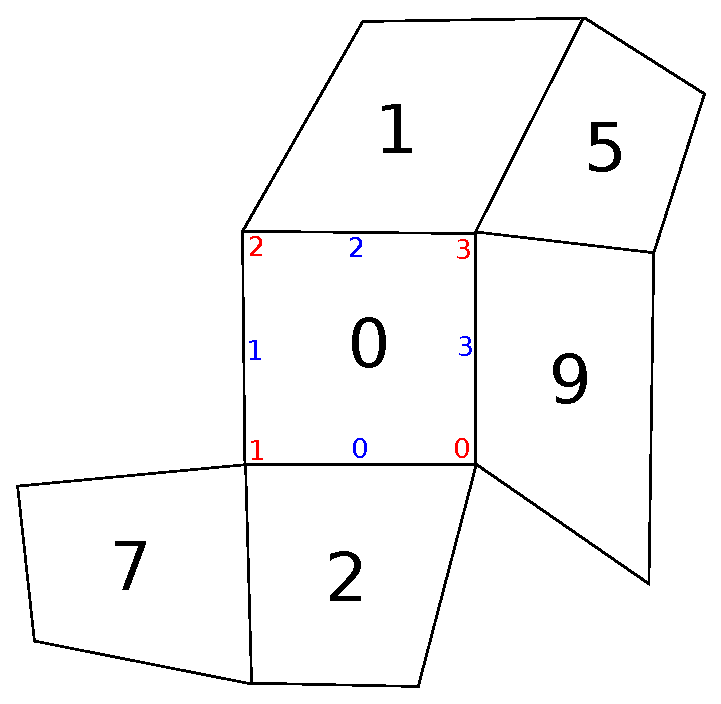
\includegraphics[scale=.45]{images/mono_cpu_main_methods_involved_eval_topology}
\caption{Example of configuration; in red local numbering of nodes, in blue local numbering of lines.}
\label{fig:mono_cpu__main_methods_involved__eval_topology}
\end{figure}

\subsubsection{reorder\_neighbors}
The neighboring elements are stored by \verb|Metis| in a not ordered way. This function reorders the neighbors in order to have the side neighboring positioned in the first four position of the neighbors vector reordered. If the reference element has less than 4 neighbors located on the edge, in the vector of the neighbors will be reported the number of the correspondent line multiplied (-1) and reduced of 1. A support vector is used as pointer to determine in which position of the vector the neighbors of the i-th corner are located.
\medskip

For example, referring to Fig.(\ref{fig:mono_cpu__main_methods_involved__eval_topology}), the reordered vector of neighboring and the vector of pointers will be:
\medskip

neighbors=[2,9,1,-4,7,5]; ptr=[4,4,5,5];

\subsubsection{set\_neighbors\_cor\_pos}
\verb|GMSH| creates a mesh orienting the elements in a pseudo random way. Considering a reference element and one of its neighbors, this function sets on which edge the reference element is located respect to the neighbor considered. In that way is possible to match uniquely the sides of the elements. This information is stored in the vector \verb|neighbor_cor_pos|, member of the class \verb|element|. It is possible to obtain this information using the method \verb|neighbor_orientation|.

\subsubsection{write\_file}
It writes all the information elaborated on each element in a \verb|.msh| format (cmp. Sec.(\ref{subsection:gmsh})). The name of the file is specified as input to the method.

\subsection{Boundary conditions}
We create a vector of vector of function pointers, called \verb|border_function_ptr|, that allows to set different boundary functions on the same region (for example, a different boundary function for each degree of freedom of the problem) or in different regions of the domain. The method \verb|set_border_function| allows the user to set these boundary functions: it takes in input the function itself, the index of the first and the last line involved, a flag referring to the type of boundary condition (\verb|DIRICHLET|, \verb|NEUMANN|, \verb|WALL|, \verb|NOCONDITION|) and the number of degree of freedom we want to set (default 1). The method \verb|get_bc_type| returns the type of the boundary condition imposed on a line while the method \verb|eval_bc| determines the value of the boundary function in a given point.

Periodicity boundary conditions deserve a particular attention. The user has to guarantee a correspondence 1 to 1 between elements periodic to each other and he must not override the line with the lower index. This condition is set using the function \verb|set_periodicity_mesh| where the lines indexes of first border are imposed in ascending order while the corresponding border is specified giving the index number of the first corresponding line and the las corresponding line. This method simply change the neighbors of the elements involved in the periodicity. Moreover it constructs the following mapping between the lines:

\begin{itemize}
\item 0, no periodic condition;
\item $i<0$, periodic with the line $-i-1$ in reverse order of the nodes;
\item $i>0$, periodic with the line $i-1$ in direct order of the nodes.
\end{itemize}

\subsection{Logical to physical transformation}\label{subsec:mapping}
It is necessary to define a transformation between a logical domain (on which the problem is solved) and the physical domain. In the following, the map from from a logical quadrangular of coordinates $[-1,1]\times[-1,1]$ to a physical one is reported:

\begin{equation}\label{eq:transf_1}
\textbf{F}_m:[-1,1]^2 \rightarrow \Omega_m \subset \mathbb{R}^2
\end{equation}
where
\begin{equation}\label{eq:transf_2}
\textbf{x}=\textbf{F}_m(\hat{\textbf{x}})= \frac{1}{4} \sum_{i=1}^{4} (1+\sigma_{\hat{x}}\hat{x})(1+\sigma_{\hat{y}}\hat{y}) \textbf{v}_i
\end{equation}
where $\textbf{x}$ are the coordinates of a point in the physical domain, $\hat{x}$ and $\hat{y}$ are the coordinates of the point in the logical domain, $\sigma_{\hat{x}}$ and $\sigma_{\hat{y}}$ are the coordinates of the reference quadrangular in the logical domain:

\begin{table}
\centering
\begin{tabular}{|c|c|}
\hline
$\sigma_{\hat{x}}$ & $\sigma_{\hat{y}}$\\
\hline
+1 & +1\\
\hline
+1 & -1\\
\hline
-1 & -1\\
\hline
-1 & +1\\
\hline
\end{tabular}
\caption{Transformation coefficients.}
\label{tab:coeff}
\end{table}

In Eq.(\ref{eq:transf_2}) the vector $\textbf{v}_i$ there are the coordinates of each vertex of a quadrangular in the physical domain. So, knowing the logical coordinate $\hat{\textbf{x}}=(\hat{x},\hat{y})$ of a point in the logical domain, it's possible reconstruct its position respect to the quadrangular of physical vertex $\textbf{v}_i$ in the physical domain. Based on this transformation, it is possible to build the Jacobian of the transformation, the determinant of the Jacobian and the inverse Jacobian. All the methods regarding the transformation from the logical domain to the physical one are implemented in the classes \verb|mapping_base| and \verb|mapping|.

\section{Parallel mesh management}\label{section:multi_CPUs}
The core part of the mesh management is contained in the class \verb|mesh_parallel| which implements all the methods necessary to obtain a good partitioning of the grid over the cluster. It is a derived class because it inherits from the class \verb|mesh|, cmp. Sec.(\ref{section:mono_cpu}). The logic behind this implementation is that all the mesh data, the I/O methods and all the methods to evaluate the topology of the mesh are implemented in \verb|mesh| which can be used alone, for a sequential code, or it becomes the base class in a parallel code. Therefore, in the case of a parallel code, each process will allocate a \verb|mesh_parallel| variable which will not contain the global informations of the mesh but only the local ones.
\medskip

In a parallel code, each process is identified by an unique positive number called $rank$. In the following we will use use the convention to call \textit{root process} the the process with $rank=0$.

\subsection{Overview of the class}\label{subsection:multi_CPU_overview}
After doing a mesh with the software \verb|GMSH|, cmp. Sec.(\ref{subsection:gmsh}), the user has to save the file in the \verb|.msh| format. The basic things that the class perform are: the class allocated on root process reads the file and loads the data in its data structures, then operates a simple pre-partitioning sending equal parts of the mesh to each process and finally operates a good partitioning redistributing the mesh over the processes. The user can decide to write on file, one for each process, the local part of the mesh obtained with the pre-partitioning and/or with the partitioning in \verb|.msh| format to avoid to recompute every time the partitioning. The constructor of the class accepts several variables to choose what the class have to do:

\begin{itemize}
 \item $1^{st}$ parameter: rank of the process;
 \item $2^{nd}$ parameter: size, therefore the number of processes available for the simulation;
 \item $3^{rd}$ parameter (default=0): number of refinements , how many times the partition  has to be refined;
 \item $4^{th}$ parameter (default=\verb|"mesh.msh"|): file name (type \verb|string|), it is the name of the input file for the mesh;
 \item $5^{th}$ parameter (default=\verb|READ_MONO|): flag that indicates the input mesh type: \verb|READ_MONO| if the root process reads the full mesh, \verb|READ_PARALLEL_PRE| if each process reads its local non optimized partitioned mesh and \verb|READ_PARALLEL_PAR| if each process reads its local optimized partitioned mesh;
 \item $6^{th}$ parameter (default=\verb|WRITE_OFF|): flag that indicates the output mesh type: \verb|WRITE_OFF| if there is no output, \verb|WRITE_PREPARTITIONING| if each process writes on file its local mesh after the pre-partitioning, \verb|WRITE_PARTITIONING| after the partitioning, \verb|WRITE_REFINEMENT| after the refinement and \verb|WRITE_ALL| after each phase. Each process save a file with is local mesh, the file name is the one given in the first parameter adding the $rank$ of the process and the suffix \textit{pre} or \textit{par} or \textit{ref} depending on the flag chosen.
 \item $7^{th}$ parameter (default=1); \verb|ncon| used as option in the function \verb|ParMETIS_V3_PartMeshKway|, cmp. Sec.(\ref{subsection:parmetis});
 \item $8^{th}$ parameter (default=2); \verb|ncommonnodes|, like parameter $7^{th}$;
 \item $9^{th}$ parameter (default=1.05): \verb|ubvecc|, like parameter $7^{th}$.
\end{itemize}
There are other 3 possible parameters to add, but the explanation will be given in the last part of this section.
\medskip

When the class is constructed, according to the constructor input variables, the mesh is partitioned over the processes and all the necessary information are evaluated therefore no methods have to be called after that. The constructor of the class \verb|mesh_parallel| performs the following operations:

\begin{enumerate}
 \item reads the mesh file using the method \verb|read_file|, class \verb|mesh.msh|;
 \item computes the mesh topology, therefore for each element it computes the surrounding squares, using the method \verb|eval_neighbors|, class \verb|mesh.msh|;
 \item sends a portion of the mesh from the root process to the other processes using the method \verb|pre_partitioning|, class \verb|mesh_parallel|;
 \item writes on file the pre-partitioned mesh using the method \verb|write_file|, class \verb|mesh.msh|;
 \item computes the new topology, like point 2;
 \item finds a better partition and redistributes the local meshes among the processes using the method \verb|partitioning|, class \verb|mesh_parallel|;
 \item computes the new topology, like point 2;
 \item writes on file the partitioned mesh, like point 4;
 \item performs some refinements using the method \verb|refinement|, class \verb|mesh_parallel|;
 \item writes on file the refined mesh,like point 4;
 \item reorders the neighbors in a proper way using the method \verb|reorder_neighbors|, class \verb|mesh|;
 \item set for each line the global index and the local position of the element that contains the line using the method \verb|eval_border|, class \verb|mesh|;
 \item set for each element its position respect to its neighbors using the method \verb|set_neighbors_cor_pos|, class \verb|mesh|;
 \item creates the mapping of the ghosts using the method \verb|create_ghosts_mapping|, class \verb|mesh_parallel|.
\end{enumerate}

It is important to notice that the methods \verb|reorder_neighbors|, \verb|eval_border|, \verb|set_neighbors_cor_pos| and \verb|create_ghosts_mapping| are used only at the end since those information are not used during the pre-partitioning, partitioning and refinement phases.

\subsection{Principal methods}\label{subsection:multi_CPU_methods}
To better understand how all these operations are performed, we now explain how the principal methods have been implemented. We use the \verb|MPI| library, cmp. Sec.(\ref{subsection:mpi}), or \verb|PETSc| library, cmp. Sec.(\ref{subsection:PETSc}),for all the methods which perform parallel communication.

\subsubsection{Pre-partitioning}
The pre-partitioning is performed by the method \verb|pre_partitioning|. The goal of this method is to split and distribute the initial mesh loaded on root process in a uniform way, from the point of view of number of elements, among all the processes. It is important to notice that only the elements are distributed among the processes while each process owns a copy of the whole \verb|nodes_list| and \verb|lines_list|. Obviously this approach is not optimal for what concern the memory usage because there are data duplications; moreover it implies a lot of communication among the processes. On the other hand, it is not necessary to find which nodes and lines has to be sent to each process, operation quite expensive, and it is not necessary to create a mapping. Finally, having a copy on each process, means that it is not necessary to compute and send these information each time that the partition changes but only during the pre-partitioning. Therefore the gain is bigger than the drawback in general; obviously,
if there are problem of memory availability, the first solution should be preferred.
\medskip

For what concerns the \verb|nodes_list|, we use the function \verb|MPI_Bcast| to send the data from the root process to the others. The sender packs the data into two different buffers: one of type \verb|double| containing the coordinates of all the nodes and the other of type \verb|int| containing their global index. The receivers unpack the buffers storing the information in their local \verb|nodes_list|. Before this step it is necessary to know the size of the buffers to send, therefore the number of nodes is broadcasted to each process. The broadcasting of the \verb|nodes_list| is exactly the same except that now the buffer is only one due to the fact that all the data are integer.
\medskip

The preliminary step for the splitting the \verb|elements_list| over the processes is to decide the destination of each element. We use a very simple method to do this: we divide the \verb|elements_list| into blocks of almost equal size each containing a consecutive sequence, considering the \verb|global_index|, of elements and each block is assigned to one process. The pros of this method are that it is very fast and simple to implement, the cons are that close indexes doesn't mean close elements because the \verb|GMSH| numbering is quite random and therefore the resulting pre-partition is usually very inefficient. It is necessary that each process knows which elements will receive, therefore we create a vector with the structure of the \verb|ParMETIS| \verb|elmdist| and we broadcast them to each process; with the information contained in the \verb|elmdist|, each process knows exactly the number and the global indexes of the elements that it will receive. Then the root process packs all the data of one
block in a buffer of \verb|int| and sends it to the corresponding process using the function \verb|MPI_Send|, while the receiving process receives the data using the function \verb|MPI_Receive| and unpacks the buffer. It is important to notice that the data contained in the buffer are always different and, since it is use only one buffer, it is necessary to use a blocking communication to avoid loss of data.
\medskip

It is necessary that each process stores not only its own elements but also the ghosts elements to evaluate in a proper way the mesh topology using the function \verb|eval_topology|. Ghost elements are the neighboring elements which do not belong to the process. They are necessary otherwise, the topology evaluation, instead of neighbors, would find border. After evaluating the ghosts, like for the elements, we scatter the number of ghosts to send and then the buffer of ghosts.
\medskip

Obviously, the root process has the data of the whole mesh therefore at the end all the elements which belongs to other process must be free.

\subsubsection{Partitioning}
In general the pre-partitioned mesh is an ensemble of disjointed clusters of elements and therefore it is quite inefficient to perform calculations on such domains because it implies a lot of communication and a consequent waste of time. For this reason it is necessary to repartition the mesh in a way that each process own only a connected cluster of elements to ensure a minimal number of ghosts elements.

The \verb|ParMETIS|, cmp. Sec.(\ref{subsection:parmetis}), function \verb|ParMETIS_V3_PartMeshKway| evaluates a better partitioning knowing the initial mapping of the elements. The output is a local mapping which maps each element to a certain process. Given this mapping the function \verb|partitioning_move_elements| physically moves the elements among the processes.
\medskip

Every process keeps a certain amount of elements and receives all the other from other processes; it is very inefficient to perform a direct substitution in its \verb|elements_list| since it is necessary to be sure not to overwrite elements which have not already been moved, otherwise it could happen a data loss. The direct substitution could be implemented storing a flag in each element to indicate if that element has already been moved or not: if it has not been moved yet, that element have to be stored in a temporary variable to avoid the overwriting.

This mechanism works but it is not very efficient because the number of elements to move is generally very large indeed it is almost the same order of magnitude of the elements present in the process. We adopt the solution to create a new \verb|elements_list| for each process to store the elements received. The previous \verb|elements_list| is destroyed and substitute with the new one at the end of all the communications. The inefficiency of this method is that it is necessary to perform a copy of the elements which are mapped in the same process. Instead of using \verb|MPI_Send| and \verb|MPI_Receive| for what concern the communication each process communicates how many elements will it send to the other process using the function \verb|MPI_Scatter| and after it sends a buffer of elements with the function \verb|MPI_Scatterv|. Each process receives the number of elements and the buffer calling the same functions. These functions are both blocking, therefore, starting for process with $rank=0$ until the
highest $rank$ one process scatters its elements and all the others receive; until process with $rank=n$ has finished to send and all the other processes have finished to receive, process with $rank=n+1$ can't start. The blocking communication is not the fastest because some processes have to idle to wait the others but it avoid problems of overwriting and data losses.
\medskip

After the scattering of the elements, in a similar way, each process scatters the ghosts.

\subsubsection{Refinement}
The mesh partitioning obtained with \verb|ParMETIS_V3_PartMeshKway| is not optimal but can be refined with the function \verb|ParMETIS_V3_RefineKway| that asymptotically converges to the optimal partitioning. This function does not work with a mesh but it is necessary to create the dual graph using \verb|ParMETIS_V3_Mesh2Dual| and than using the output dual graph as input of the refinement function. As seen before, the re-mapping provided by \verb|ParMETIS| is used by the method \verb|partitioning_move_elements| to physically move the elements among the processes.

Since \verb|ParMETIS_V3_RefineKway| is an iterative algorithm which can be called an arbitrary amount of time, it is necessary to recompute the mesh topology and the \verb|elmdist| each time at the end of each iteration.

\subsubsection{Ghosts' Mapping}\label{subsection:ghost_mapping}
Each process stores only a certain part of the mesh, therefore it is necessary to have a way to know which process owns a certain information. To perform this task it is required to have a mapping. There are in general two types of mapping:

\begin{itemize}
\item \textit{local to global}: it returns the global index knowing the local index;
\item \textit{global to local}: it returns the process and the local index knowing the global index;
\end{itemize}

Since each element contains its global index, the local to global mapping is already present. Instead, for what concern the local to global one, it is necessary to know it only for the ghost elements. The method \verb|create_ghosts_mapping| create this mapping which consists, for each ghost, in the rank of the process which stores the element and its local position. The evaluation of this mapping is very simple since it is based on the class \verb|ghost_communicaton|: each process set for each elements its own rank and the local position and then the class perform all the necessary communication. Each process stores its mapping in a vector and it is possible to know the rank and the position of a certain ghost using the functions \verb|get_ghosts_rank| and \verb|get_ghosts_pos|.

\subsubsection{Set Periodicity condition}\label{subsection:set_periodicity}
The periodicity condition when it is set for a parallelized mesh is slightly different from the sequential case since it is possible that the periodic elements are stored partly or completely in an other process. The function \verb|set_periodicity| first call the function \verb|set_periodicty_mesh| of the class \verb|mesh| which add all periodic elements like ghosts if they are not locally stored and change simply the neighbors information for the others. But this method add these ghosts with only the information of their global index because when it is used only on a single process there will be no need to add new ghosts since the process stores all the mesh. Therefore the function, in the parallel class, use the class \verb|ghost_communicaton| to obtain all the information needed for this new ghosts, namely the vertex global index. This operation is performed simply setting on each process and for each elements the four vertex information and storing the ghosts values after the class has performed the
communication.

\subsection{Class ghost\_communication}\label{subsection:ghost_communication}
The class mesh contains as member a pointer to the class ghost\_communication. This class has the purpose of providing methods to update the values needed in ghost elements. It relies completely on \verb|PETSc| functions which will be explain in detail in  Sec.(\ref{subsection:PETSc}).

The class is built in a way that it is easily possible to change the amount of data which has to be communicated per element by the call of a single function. This is a very desirable feature, because it can be used for different purpose and the user doesn't have to deal with \verb|PETSc| functions every time. In fact the constructor creates the local \verb|PETSc| vec which will contain the values on the processor and the ghost values after being updated. Then it is mandatory to call the function \verb|set_size| before using it the first time and every time one wants to change the number of values per element. This function calls first \verb|set_idxs| which sets the arrays of indices needed by the \verb|PETSc| function \verb|VecCreateGhost|, which is called right after, and needed to set local values and retrieve local ghost values. In this way a global ghosted vector is created.

To update ghost values it is sufficient to call the function \verb|set_global_vec| passing to it a vector of local values which contains the values for the actual elements on the processor. This functions contains the calls to \verb|PETSc| functions:

\begin{itemize}
\item \verb|VecSetValues|;
\item \verb|VecAssemblyBegin|;
\item \verb|VecAssemblyEnd|;
\item \verb|VecGhostUpdateBegin|;
\item \verb|VecGhostUpdateEnd|;
\item \verb|VecGhostGetLocalForm|;
\item \verb|VecGetValues|;
\item \verb|VecGhostRestoreLocalForm|.
\end{itemize}

After this sequence the private member \verb|ghost_values| contains the updated values and to retrieve them it is possible to call the public functions \verb|get_ghosts_values| to obtain a reference to all the vector and  \verb|get_ghosts_value| to obtain a reference to the element specified during the call.

The implementation allows the user to communicate only \verb|double| values.

It is also possible to specify two indices of the local vector,where to start and end to fill the global \verb|PETSc| Vec.

The function \verb|free| is provided to free the memory from \verb|PETSc| variables when not needed anymore.

\section{Libraries and tools}\label{section:lib}
In this section different libraries and free software used for the code are explained.

The mesh generation is performed using \verb|GMSH|, while \verb|METIS| and \verb|ParMETIS| are used to evaluate neighboring squares and compute an optimized partitioning of the elements among the processes.

\verb|MPI| is used to actually send data to processes according to the partitioning previously computed.

\verb|PETSc| provides the functions to update ghosts' values and it is used to obtain information about periodic ghost elements.

Functions of interest are shown for each library and the logic behind their algorithms is analyzed.

\subsection{GMSH}\label{subsection:gmsh}
The mesh is generated with the free software \verb|GMSH|. This software is a tool to create meshes in both bi-dimensional and tri-dimensional domains. In this section we give a little presentation of the software. For further information cmp. \cite{gmsh_man} and \cite{gmsh_art}.

Before explaining the software some useful definitions are given:

\begin{itemize}
\item \textit{Structured grid}: grid built with a tassellation of n-dimensional Euclidean space by congruent parallelotopes\cite{wolfram_struct}.
\item \textit{Unstructured grid}: tassellation of an Euclidean domain by simple shapes in irregular pattern.
\item \textit{Conformal grid}: grid where each node of each element is in correspondence of nodes of other elements. In such a grids there are no nodes on element edges.
\item \textit{Unconformal grid}: nodes on elements edges are allowed.
\end{itemize}

The software allows the drawing of a geometry as set of points and lines which connect these points. Once the geometry is drawn as a closed set of lines it is sufficient to create a plane surface inside it and then generate the mesh. It is also possible to give the initial geometry as input if one knows the \verb|GMSH| format, which will be explained later. In fact it is possible to write a textfile in the format \verb|.msh| in which only the points, or the points and the lines connecting them are written. \verb|GMSH| can read this kind of files and build up the initial geometry on which the mesh is then generated.

For the purpose of this work we used only meshes which contain quadrangular elements. In our code we use always a clockwise ordering of the vertexes of each element. To respect this convention, it is necessary to draw the geometry using a clockwise sense.

\verb|GMSH| gives the possibility to choose between three different algorithms for the creation of the first coarse mesh. In each of them a Delaunay mesh that contains all the points of the initial geometry is first constructed using a divide-and-conquer algorithm. Missing edges are recovered using edge swaps. After this initial step three different algorithms can be applied to generate the final mesh:

\begin{itemize}
\item \textit{Delaunay} algorithm in which new points are inserted sequentially at the circumcenter of the element that has the largest adimensional circumradius. The mesh is then reconnected using an anisotropic Delaunay criterion.
\item \textit{MeshAdapt} algorithm is based on local mesh modifications. This technique makes use of edge swaps, splits, and collapses: long edges are split, short edges are collapsed, and edges are swapped if a better geometrical configuration is obtained.
\item \textit{Frontal} algorithm is inspired by the work of S. Rebay, which is based on a Delaunay triangulation, but computes simultaneously point positions and connections.
\end{itemize}

The three different algorithms are ranked in Tab.(\ref{tab:rank}):

\begin{table}
\centering
\begin{tabular}{|l|c|c|c|}
\hline
 & Robustness & Performance & Element quality\\
\hline
\verb|MeshAdapt| & 1 & 3 & 1\\
\hline
\verb|Delaunay| & 2 & 1 & 2\\
\hline
\verb|Frontal| & 3 & 2 & 1\\
\hline
\end{tabular}
\caption{Algorithms ranking.}
\label{tab:rank}
\end{table}

All these algorithms produce triangular elements, which are then subdivided in quadrangular connecting the center of each of them with all middle points of the edges, therefore all triangles are subdivided in quadrangles.

The same procedure is also applied when one want to refine the mesh: it is possible to use the \textit{Refine by Splitting} tool to build four elements from each element of the previous mesh. Each refinement will contain four times the elements than the previous one.

Since the algorithm always connects the center with the middle points of the edges it maintains the conformity of the mesh and creates block structured meshes.

A simple example of mesh generated with this software is shown in Fig.(\ref{fig:simple_mesh}).

\begin{figure}
\centering
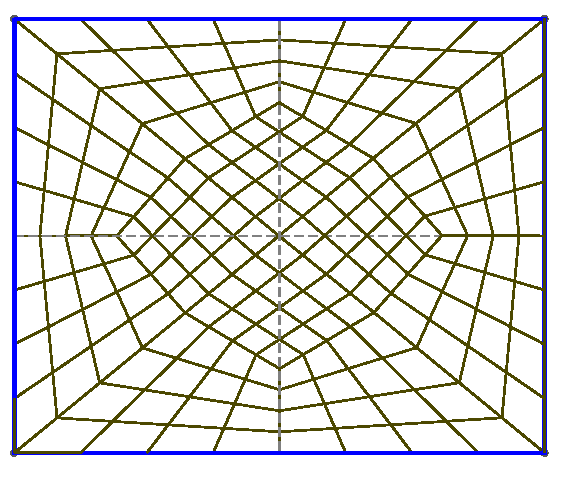
\includegraphics[scale=.6]{images/simple_mesh.pdf}
\caption{GMSH mesh generation example, using Delaunay algorithm.}
\label{fig:simple_mesh}
\end{figure}

\subsubsection{GMSH file format}\label{subsubsection:gmsh_format}
The mesh is stored in a \verb|.msh| file, which is written in \verb|ASCII| format. This type of file is subdivided in sections, which are separated by flags of begin and end.

The first section is mandatory and it starts with the flag \verb|\$MeshFormat|. It contains on the  same row:

\begin{itemize}
\item \textit{version of the format};
\item \textit{type of the file};
\item \textit{data size}.
\end{itemize}

It is ended with the flag \verb|\$EndMeshFormat|.

The second section contains the information on nodes. It begins with the line \verb|\$Nodes|. On the next line there is the total number of nodes,and each of the following lines contains:

\begin{itemize}
\item \textit{global index} of the node;
\item \textit{coordinates} of the node.
\end{itemize}

The section ends with the line \verb|\$EndNodes|.

The next section begins with \verb|\$Elements| and contains the initial points used to build the mesh, the lines connecting these points and the list of elements of the mesh. The first line contains the sum of the total numbers of these three things.  Every element is stored in a line, and for each of them it is possible to find:

\begin{itemize}
\item \textit{global index} of the element;
\item \textit{type of element}: typically this value is 15 for points, 1 for lines, 2 for triangles and 3 for quadrangles;
\item \textit{number of tags}: an integer number which denotes how many of the following numbers are tags which give additional informations;
\item \textit{tags}: by default, the first tag is the number of the physical entity to which the element belongs; the second is the number of the elementary geometrical entity to which the element belongs; for the lines this tag will be used to assign border conditions; the third is the number of mesh partitions to which the element belongs, followed by the partition ids (negative partition ids indicate ghost cells). A zero tag is equivalent to no tag.
\item \textit{global indexes} of the corner nodes of the element.

\end{itemize}

\verb|GMSH| can compute a partition, but we decided to implement our on code to do that, to have more flexibility. Also, the computational cost of the partition is very high, so it is better to perform it on multi processors.

\subsection{METIS}\label{subsection:metis}
\verb|METIS| is a serial software package for partitioning large irregular graphs, partitioning large meshes, and computing fill-reducing orderings of sparse matrices developed at the 	\textit{Department of Computer Science and Engineering} at the \textit{University of Minnesota}.

Since the parallel version, \verb|ParMETIS| is very similar and it is more used in the code, some of the logic behind the algorithms will be explained in the next section. Only the called function will be explained here. For more information cmp. \cite{metis}.

\verb|METIS| is called only to compute neighboring squares for each element using the function \verb|METIS_MeshToDual|. The function contains a quite fast algorithm to compute neighbors, but but we don't know its exact complexity. The function transform a mesh into its dual graph, giving as output the adjacency of the graph. From this it is possible to obtain the neighbors of each element. Inputs of the function are:

\begin{itemize}
\item \verb|ne|, number of elements in the mesh;
\item \verb|nn|, number of nodes in the mesh;
\item \verb|eptr|, \verb|eind|, a pair of arrays storing the mesh. This two arrays are correlated: \verb|eptr| contains indexes of \verb|eind|. \verb|eind| contains global indexes of nodes. The ith element of \verb|eptr| is the index of \verb|eind| from where the nodes of the ith element of the mesh start. So \verb|eind| will contain the node of element $i$ from position \verb|eptr[i]| until position \verb|eptr[i+1]|.
\item \verb|ncommon| specifies the minimum number of nodes that two elements have to be in common to be considered as neighbors. It may be 1 or 2 for quadrangular elements. In this case a value of 1 is used since also the corner neighbors have to be evaluated;
\item \verb|numflag| denotes the style of numbering order. For C-style it has the value of 0, hence here is set to zero.
\end{itemize}

Outputs are:

\begin{itemize}
\item \verb|xadj|,\verb|adjncy|: this two arrays have similar structures of \verb|eptr| and \verb|eind|: the ith value of \verb|xadj| contains the index of \verb|adjncy| where the indexes of the neighboring squares of the ith element start.
\end{itemize}

\subsection{ParMETIS}\label{subsection:parmetis}
The parallel version of \verb|METIS| is \verb|ParMETIS| and it is called to perform the partition optimization. Information about the library are taken from \cite{parmetis}. \verb|ParMETIS| is an \verb|MPI|-based (cmp. Sec.(\ref{subsection:mpi})) parallel library that implements a variety of algorithms for partitioning and repartitioning unstructured graphs and for computing fill-reducing orderings of sparse matrices.

Fig.(\ref{fig:parmetis_diagram}) shows an overview of the functionality provided by \verb|ParMETIS| as well as a guide to its use.

\begin{figure}
\centering
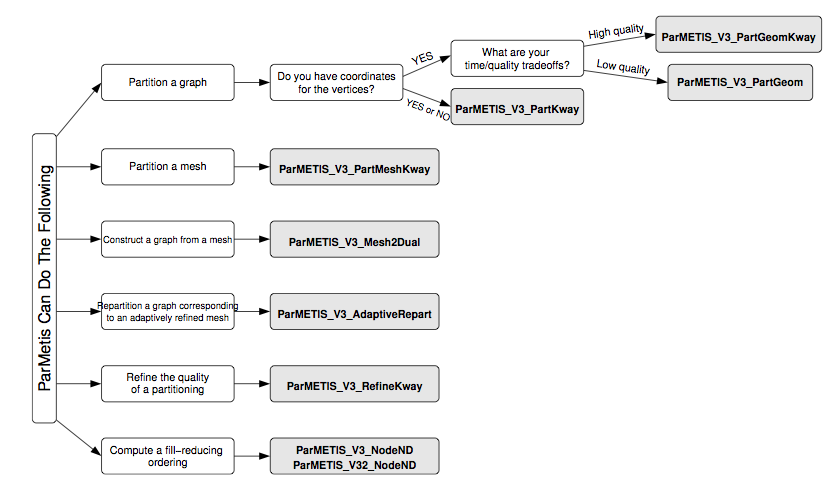
\includegraphics[scale=.45]{images/parmetis.png}
\caption{Functionality of ParMETIS.}
\label{fig:parmetis_diagram}
\end{figure}

The function used to perform the partition optimization is \verb|ParMETIS_V3_PartMeshKway|. Since the algorithm contained in \verb|ParMETIS| can only partition graphs, this function contains a call to \verb|ParMETIS_V3_Mesh2Dual| and then a call to the function \verb|ParMETIS_V3_PartKway|. In this way the dual graph of the mesh is created and then is partitioned using a serial multilevel k-way partitioning algorithm.

This algorithm has been shown to quickly produce partitioning that are of very high quality. It consists of three phases: graph coarsening, initial partitioning, and uncoarsening/refinement. In the graph coarsening phase, a series of graphs is constructed by collapsing together adjacent vertices of the input graph in order to form a related coarser graph. Computation of the initial partitioning is performed on the coarsest (and hence smallest) of these graphs, and so it is very fast. Finally, partition refinement is performed on each level graph, from the coarsest to the finest (i.e., original graph) using a KL/FM-type refinement algorithm.

Fig.(\ref{fig:parmetis_algorithm}) illustrates the multilevel graph partitioning algorithm.

\begin{figure}
\centering
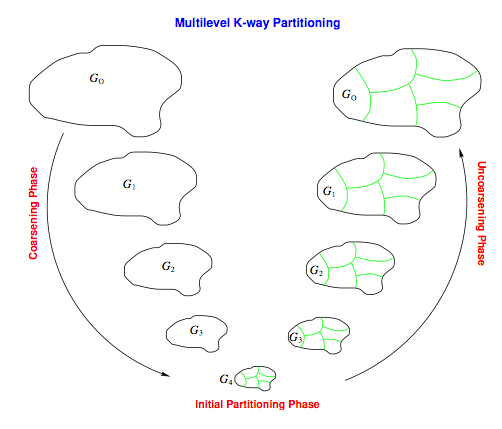
\includegraphics[scale=.45]{images/parmetis_algorithm.png}
\caption{Multilevel K-way partitioning algorithm.}
\label{fig:parmetis_algorithm}
\end{figure}

\verb|ParMETIS_V3_Mesh2Dual| is  used for the refinement. Infact \verb|ParMETIS| can only perform partitioning refinements on graphs, so the sequence \verb|ParMETIS_V3_Mesh2Dual| \verb|ParMETIS_V3_RefineKway| is called for each refinement.

It follows a little explanation of inputs and outputs of the functions used.

\subsubsection{PartMeshKway}\label{subsubsection:partmeshkway}
The function accepts as input a pre-partitioned mesh and returns as output the total number of cut edge in the partition and an array which contains a mapping between elements and processes where they have to be sent.

The pre-partitioned mesh that must be put as input has a different format from the one stored in the code. It is constituted by three arrays:

\begin{itemize}
\item \verb|elmdist| is an array equal in each process and contains the number of elements in each process. The length of \verb|elmdist| is equal to the number of the processes plus one, because each element in \verb|elmdist| denotes the first of the elements on that process, so the last number of \verb|elmdist| is the last element on the last process plus one;
\item \verb|eptr| and \verb|eind| are arrays different in each process. The meaning is exactly the same as described for \verb|METIS| function.
\end{itemize}

The function accepts other inputs:

\begin{itemize}
\item \verb|elmwgt| is a local array of length equal to the length of the local element list and stores the weights for the elements. How this array is obtained will be discussed in detail later.
\item \verb|wgtflag| is a flag which can assume two values: 0 if the partition has to be performed without weights (\verb|elmwgt| is \verb|NULL|), 2 if weights are on vertexes only;
\item \verb|numflag| has the same meaning as in \verb|METIS| function;
\item \verb|ncon| is the number of vertex which every node has (for multiphysics problems);
\item \verb|ncommonnodes| specifies the minimum number of nodes that two elements must have in common to be considered as neighbors. It may be 1 or 2 for quadrangular elements;
\item \verb|nparts| specifies the number of sub-domains desired. In this case it is equal to the number of the processes;
\item \verb|tpwgts| is an array of size \verb|ncon| x \verb|nparts| which specifies the fraction of weights that has to be assigned to each sub-domain. If the distribution has to be uniform each element of this array will have a value of 1/\verb|nparts|;
\item \verb|ubvec| is an array of size \verb|ncon| and specifies the imbalance for each constraint. A value of 1.05 is recommended and used in the code;
\item \verb|options| is an array of integer used to pass some parameters to the routine. Since here this parameters are not used, the first value of options is set to zero and this says to the routine that no options are passed;
\item a pointer to the communicator. Here it is a pointer to \verb|MPI_COMM_WORLD|.
\end{itemize}

The outputs of the function are:

\begin{itemize}
\item \verb|edgecut| contains the number of cut edges;
\item \verb|partition| is an array which contains the ranks of the processes where the elements have to be sent.
\end{itemize}

\subsubsection{Mesh2Dual}\label{subsubsection:mesh2dual}
This function takes in input a mesh with the same format of the previous one, and gives as output the connectivity of the corresponding dual graph. Inputs are:

\begin{itemize}
\item \verb|elmdist|;
\item \verb|eptr|,\verb|eind|;
\item \verb|numflag|;
\item \verb|ncommonnodes|;
\item a pointer to \verb|MPI_COMM_WORLD|.
\end{itemize}

The outputs are the following:

\begin{itemize}
\item \verb|xadj|,\verb|adjncy| with the same meaning as in \verb|METIS| function.
\end{itemize}

\subsubsection{RefineKway}\label{subsubsection:refinekway}
This function take as input a partitioned graph and refines the partition optimizing the number of ghost--cells for each process. As output it gives the rank of the process where each vertex has to be sent. Since the code gives as input the dual graph of a mesh, the output will be the rank of the process where each element (associated to a vertex in the dual graph) has to be sent. As inputs it requires:

\begin{itemize}
\item \verb|vtxdist|: this array has the same function of \verb|elmdist| and specifies how many vertices are stored on each process. The ith element of the array contains the cumulative of the element on the previous processes plus one. The length of the array is equal to the number of the processes plus one;
\item \verb|xadj|,\verb|adjncy|;
\item \verb|vwgt|,\verb|adjwgt| arrays store the weights on vertices and edges;
\item \verb|ncon|;
\item \verb|nparts|;
\item \verb|wgtflag| now can also assume values 1 or 3: 1 if weights are on edges only (\verb|vwgt| is \verb|NULL|), 3 if weights are on both vertices and edges. If it assumes value 2 (weights on vertices only) \verb|adjwgt| is \verb|NULL|;
\item \verb|numflag|;
\item \verb|tpwgts|;
\item \verb|ubvec|;
\item \verb|options|;
\item a pointer to \verb|MPI_COMM_WORLD|.
\end{itemize}

Outputs are:

\begin{itemize}
\item \verb|edgecut|;
\item \verb|partition|;
\end{itemize}

\verb|ParMETIS_V3_RefineKway| can be called repeatedly to further improve the partitioning. However, each successive call will tend to produce smaller improvements in quality.

\subsection{MPI}\label{subsection:mpi}
\verb|MPI| is a \textit{message-passing library interface specification}; for a complete reference to the library cmp. \cite{mpi}. Here we give some information extracted from the manual to explain how the library works. It addresses primarily the message--passing parallel programming model, in which data is moved from the address space of one process to that of another process through cooperative operations on each process. \verb|MPI| is a specification, not an implementation; there are multiple implementations of \verb|MPI|. This specification is for a library interface; \verb|MPI| is not a language, and all \verb|MPI| operations are expressed as functions, subroutines, or methods. It includes point--to--point message--passing, collective communications, group and communicator concepts, process topologies, environmental management, process creation and management, one--sided communications, extended collective operations, external interfaces, I/O, some miscellaneous topics, and a profiling interface.

In the code \verb|MPI| is used to broadcast on each process initial information about the nodes, to send and receive elements information according to different partitioning, and to gather on root process and then send again on each process other information about the partitioning.

All the functions used are blocking. A procedure is blocking if return from the procedure indicates the user is allowed to reuse resources specified in the call. Some functions involve point--to--point communication as  \verb|MPI_Send| and \verb|MPI_Recv|, while the others are collective. The formers may be called only on particular processes, while the latter have to be called at the same moment on each process of the same communicator. Collective calls over the same communicator must be executed in the same order by all members of the process group.

It follows a short explanation of all the functions used.

\subsubsection{MPI\_Send}\label{subsubsection:send}
\verb|MPI_Send| is a point--to--point blocking function. It is used to send data from a particular process to another particular one. It accepts the following inputs:

\begin{itemize}
\item \verb|buf|, the initial address of send buffer;
\item \verb|count|, number of elements in send buffer;
\item \verb|datatype|, type of each send buffer elements (\verb|MPI_DATATYPE|);
\item \verb|dest|, rank of destination;
\item \verb|tag|, message tag (integer);
\item \verb|comm|, \verb|MPI| communicator.
\end{itemize}

\subsubsection{MPI\_Recv}\label{subsubsection:recv}
Each time data are sent to a specific process this process must call this function to receive the buffer of data. The function accepts the followings:

\begin{itemize}
\item \verb|buf|, the initial address of send buffer;
\item \verb|count|, number of elements in send buffer;
\item \verb|datatype|, type of each send buffer elements (\verb|MPI_DATATYPE|);
\item \verb|source|, rank of source or \verb|MPI_ANY_SOURCE|;
\item \verb|tag|, message tag or \verb|MPI_ANY_TAG| (integer);
\item \verb|comm|, \verb|MPI| communicator;
\end{itemize}

Outputs are:

\begin{itemize}
\item \verb|buf|, the initial address of send buffer;
\item \verb|status|, status object.
\end{itemize}

\subsubsection{MPI\_Bcast}\label{subsubsection:bcast}
\verb|MPI_Bcast| is a collective blocking function. It's goal is to send the same data from a single process to each process of the communicator. The logic is outlined in Fig.(\ref{fig:bcast}).

\begin{figure}
\centering
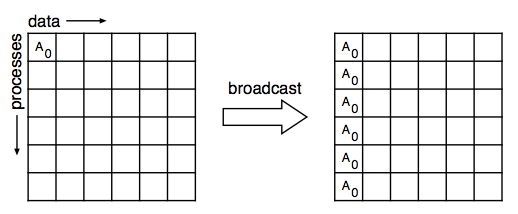
\includegraphics[scale=.45]{images/broadcast.png}
\caption{MPI\_Bcast logic.}
\label{fig:bcast}
\end{figure}

The function accepts the followings:

\begin{itemize}
\item \verb|buf|, starting address of the buffer; it is an input on root processor and an output on the other ones.
\item \verb|count|, number of elements in buffer;
\item \verb|datatype|, type of each send buffer elements (\verb|MPI_DATATYPE|);
\item \verb|root|, rank of broadcast root;
\item \verb|comm|, \verb|MPI| communicator.
\end{itemize}

\subsubsection{MPI\_Scatter}\label{subsubsection:scatter}
\verb|MPI_Scatter| is a collective blocking function. It is used to send from root process to each other process a different part of a buffer. All the parts have the same size. The logic and the one of gather function are specified in Fig.(\ref{fig:scatter_gather}).
\begin{figure}
\centering
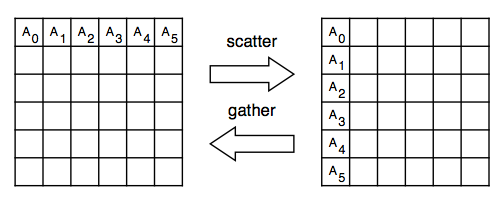
\includegraphics[scale=.45]{images/scatter_gather.png}
\caption{MPI\_Bcast logic.}
\label{fig:scatter_gather}
\end{figure}

The function requires the followings:

\begin{itemize}
\item \verb|sendbuf|, address of send buffer;
\item \verb|sendcount|, number of elements send to each process;
\item \verb|sendtype|, type of each sent buffer elements (\verb|MPI_DATATYPE|);
\item \verb|recvbuf|, address of receive buffer;
\item \verb|recvcount|, number of elements in receive buffer;
\item \verb|recvtype|, data type of receive buffer elements (\verb|MPI_DATATYPE|);
\item \verb|root|, rank of broadcast root;
\item \verb|comm|, \verb|MPI| communicator.
\end{itemize}

The output is:

\begin{itemize}
\item \verb|recvbuf|, address of receive buffer;
\end{itemize}

\subsubsection{MPI\_Scatterv}\label{subsubsection:scatterv}
It has the same logic of \verb|MPI_Scatter|, but it is possible to specify how many elements send to each process. Only two parameters change from the previous function:

\begin{itemize}
\item \verb|sendcounts|, non-negative integer array (of length group size) specifying the number of elements to send to each rank;
\item \verb|displs|, integer array(of length group size). Entry i specifies the displacement (relative to \verb|sendbuf|) from which to take the outgoing data to process $i$.
\end{itemize}

\subsubsection{MPI\_Gather}\label{subsubsection:gather}
This function has the goal to gather data coming from different processes on a single process. The logic is shown in Sec.(\ref{subsubsection:scatter}) paragraph. It accepts the same parameters as \verb|MPI_Scatter|.

A further explanation is given in Fig.(\ref{fig:gather})

\begin{figure}
\centering
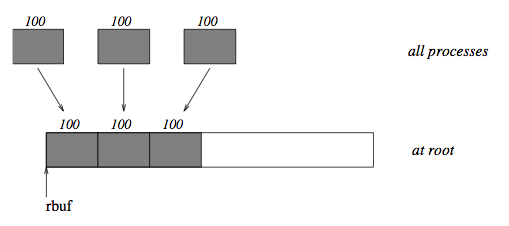
\includegraphics[scale=.45]{images/gather.png}
\caption{MPI\_Gather logic.}
\label{fig:gather}
\end{figure}

\subsection{PETSc}\label{subsection:PETSc}
\verb|PETSc|, \textit{Portable, Extensible Toolkit for Scientific Computation} is a suite of data structures and routines that provide the building blocks for the implementation of large scale application codes on parallel (and serial) computers. The information reported here are taken from \cite{petsc}. Compare it for additional guidelines.

It is a hierarchically organized library, which, by using an object-oriented programming, enables users  to employ the level of abstraction that is most appropriate for a particular problem, providing enormous flexibility. \verb|PETSc| uses \verb|MPI| standard for all message-passing communication.

The library contains modules to deal with:

\begin{itemize}
\item index sets (\verb|IS|), including permutations, for indexing into vectors, renumbering, etc;
\item vectors (\verb|Vec|);
\item matrices (\verb|Mat|) (generally sparse);
\item managing interactions between mesh data structures and vectors and matrices (\verb|DM|);
\item over fifteen Krylov subspace methods (\verb|KSP|);
\item dozens of preconditioners, including multi-grid, block solvers, and sparse direct solvers (\verb|PC|);
\item nonlinear solvers (\verb|SNES|);
\item time steppers for solving time-dependent (nonlinear) PDEs, including support for differential algebraic equations (\verb|TS|).
\end{itemize}

In this section we explain the functions used in the class \verb|ghost_communication|.

\subsubsection{VecCreate}\label{subsubsection:VecCreate}
This is the general function to create an empty vector without any type. Input parameters:

\begin{itemize}
\item \verb|comm| - the communicator for the vector object.
\end{itemize}
Output parameters:
\begin{itemize}
\item \verb|vec| - a pointer to the vector object.
\end{itemize}

\subsubsection{VecCreateGhost}\label{subsubsection:VecCreateGhost}
Creates a parallel vector with ghost padding on each processor. Input parameters:

\begin{itemize}
\item \verb|comm| - the communicator to use;
\item \verb|n| - local vector length;
\item \verb|N| - global vector length (or \verb|PETSC_DECIDE| if \verb|n| is given);
\item \verb|nghost| - number of local ghost points;
\item \verb|ghosts| - array of global indices of ghost points.
\end{itemize}

Output parameters:

\begin{itemize}
\item \verb|vv| - a pointer to the global vector representation (without ghost points as part of vector).
\end{itemize}

\subsubsection{VecSetValues}\label{subsubsection:VecSetValues}
Inserts or adds values into certain locations of a vector. Input parameters:

\begin{itemize}
\item \verb|x| - vector to insert in;
\item \verb|ni| - number of elements to add;
\item \verb|ix| - array of indexes where to add;
\item \verb|y| - array of values;
\item \verb|iora| - insert mode (\verb|INSERT_VALUES| or \verb|ADD_VALUES|).
\end{itemize}

\subsubsection{VecAssemblyBegin and VecAssemblyEnd}\label{subsubsection:VecAssembly}
The former begins and the latter ends to assembly a vector. This routines should be called in sequence after completing a call to \verb|VecSetValues|. Input parameters:

\begin{itemize}
\item \verb|vec| - the vector.
\end{itemize}

\subsubsection{VecGhostUpdateBegin and VecGhostUpdateEnd}\label{subsubsection:VecGhostUpdate}
The former begins and the latter ends the vector scatter to update the vector from local representation to global or global representation to local. They should be called in sequence after having updated the local or global vector. Input parameters:

\begin{itemize}
\item \verb|g| - the vector;
\item \verb|insertmode| - \verb|ADD_VALUES| or \verb|INSERT_VALUES|;
\item \verb|scattermode| - \verb|SCATTER_FORWARD| or \verb|SCATTER_REVERSE|.
\end{itemize}

\subsubsection{VecGhostGetLocalForm and VecGhostRestoreLocalForm}\label{subsubsection:VecGhostGetLocalForm}
Obtains the local ghosted representation of a parallel vector. Input parameters:

\begin{itemize}
\item \verb|g| - the global vector.
\end{itemize}
\begin{itemize}
\item \verb|l| -a pointer to the local ghosted representation.
\end{itemize}

\subsubsection{VecGhostRestoreLocalForm}\label{subsubsection:VecGhostRestoreLocalForm}
Restores the local ghosted representation of a parallel vector after being used. Input parameters:

\begin{itemize}
\item \verb|g| - the global vector;
\item \verb|l| - a pointer to the local ghosted representation.
\end{itemize}

\subsubsection{VecGetValues}\label{subsubsection:VecGetValues}
Gets values from certain locations of a vector. Can only get values on the same processor. Input parameters:

\begin{itemize}
\item \verb|x| - vector to get the values from;
\item \verb|ni| - number of elements to get;
\item \verb|ix| - array of indices where to get them from (in global 1d numbering).
\end{itemize}

Output parameters:

\begin{itemize}
\item \verb|y| - array of values.
\end{itemize}

\subsubsection{PetscFree}\label{subsubsection:PetscFree}
Frees memory. Input parameters:

\begin{itemize}
\item \verb|memory| - memory to free.
\end{itemize}

\subsubsection{VecDestroy}\label{subsubsection:VecDestroy}
Destroys a vector. Input parameters:

\begin{itemize}
\item \verb|v| - a pointer to the vector.
\end{itemize}

\section{Examples}\label{section:mesh_ex}
Now we report two examples in which we test the performance of this part of the code. In the first example, Sec.(\ref{subsection:Tokamak_section}) we mesh the Scrape of Layer (SOL) and the internal part of the toroidal section of a Tokamak.In the second one, Sec.(\ref{subsection:mirror_machine}) we mesh the interior part of the mirror machine following the magnetic field lines.

\subsection{Tokamak section}\label{subsection:Tokamak_section}
As explained previously (cmp. Sec(\ref{subsection:gmsh})) \verb|GMSH| allows the user to build the mesh on the domain using different algorithms; in particular it's possible to choose as option an algorithm based on a \textit{frontal} approach, or a \textit{Delaunay} or a \textit{mesh adaptation} one. As it is possible to see in Fig.(\ref{fig:mesh}) the density of elements is higher in the upper  and the lower part of the domain: this is due to the fact \verb|GMSH| builds an higher number the elements where the density of points on the border of the domain is higher. In this particular example the \textit{frontal} and the \textit{mesh adaptation} algorithms seem to build a mesh in which the distribution of elements is more uniform.
\medskip

In the following figures the part of the code regarding the management of the grid as been run on four process using a finer grid (11746 elements) built using a mesh adaptation algorithm. The Fig.(\ref{fig:prepartitioning}) shows the results obtained at the first step of the distribution of the elements on the processes pre-partitioning as been implemented simply dividing the list of elements in almost equal part on each process. GMSH creates a pseudo-random numbering of the elements: so, on each process, a disjointed domain is created (cmp Fig.(\ref{fig:prepartitioning})). In Fig.(\ref{fig:partitioning}) the new redistribution of elements among processes is reported: on each process part the domain is reconstructed using \verb|ParMetis|, creating a non-disjointed domain. The four domain seem to be different: the partitioning has been constructed using a uniform distribution of the \verb|weights|, so almost the same number of elements has been associated to each processor. In the last Fig.(\ref{fig:refinement}) we performed 5 refinements of the mesh partitioning.

\begin{figure}
\centering
\subfigure[{Frontal: 4197 elements}\label{fig:tokamak_layer_frontal}]
{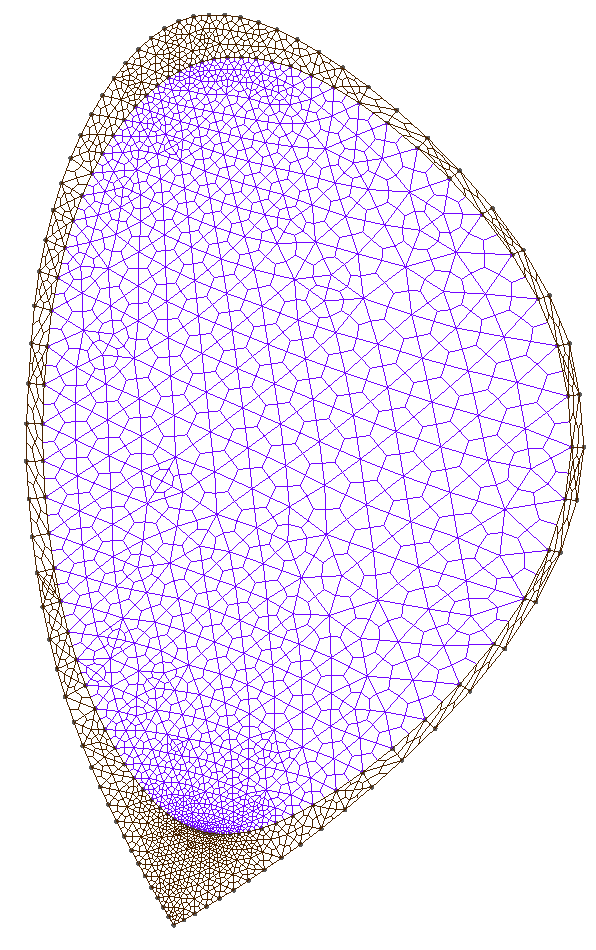
\includegraphics[scale=.55]{images/tokamak_layer_frontal.pdf}}\quad\quad
\subfigure[{Delaunay: 4803 elements.}\label{fig:tokamak_layer_delaunay}]
{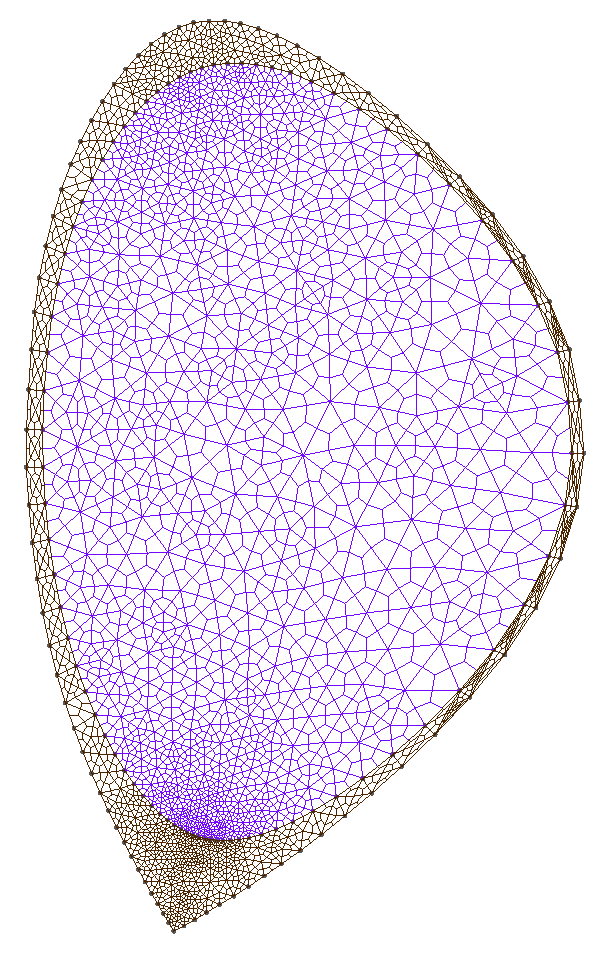
\includegraphics[scale=.55]{images/tokamak_layer_delaunay.pdf}}\quad\quad
\subfigure[{Mesh adaptation: 3213 elements}\label{fig:tokamak_layer_mesh_adapt}]
{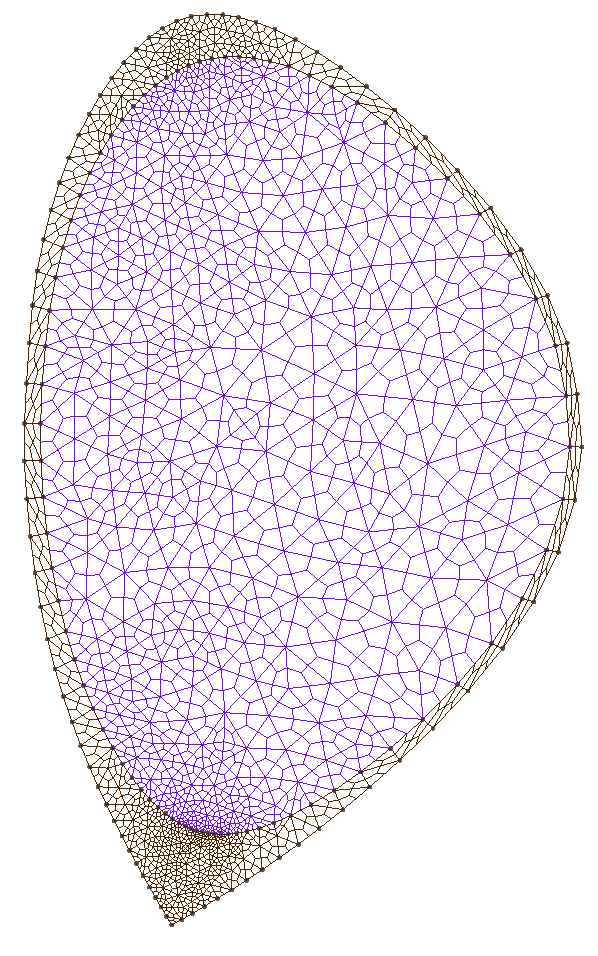
\includegraphics[scale=.55]{images/tokamak_layer_mesh_adapt.pdf}}
\caption{Mesh creation options of a Tokamak section.}\label{fig:mesh}
\end{figure}

\begin{figure}
\centering
\subfigure[{rank = 0}\label{fig:tokamak_layer_mesh_adapt_fine_0_pre}]
{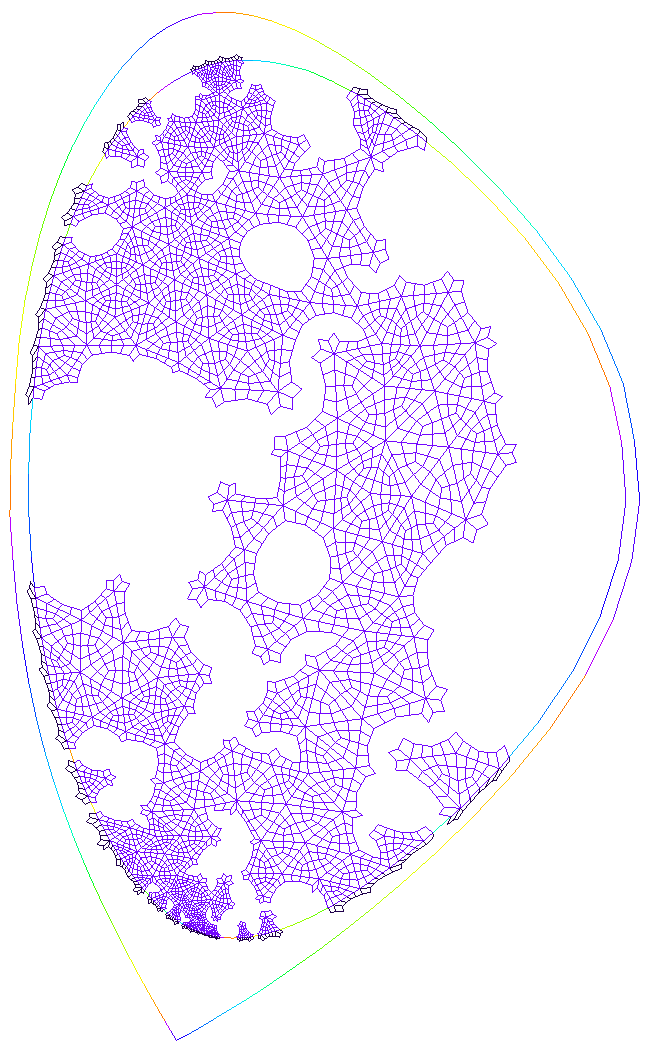
\includegraphics[scale=.5]{images/tokamak_layer_mesh_adapt_fine_0_pre.pdf}}\quad
\subfigure[{rank = 1}\label{fig:tokamak_layer_mesh_adapt_fine_1_pre}]
{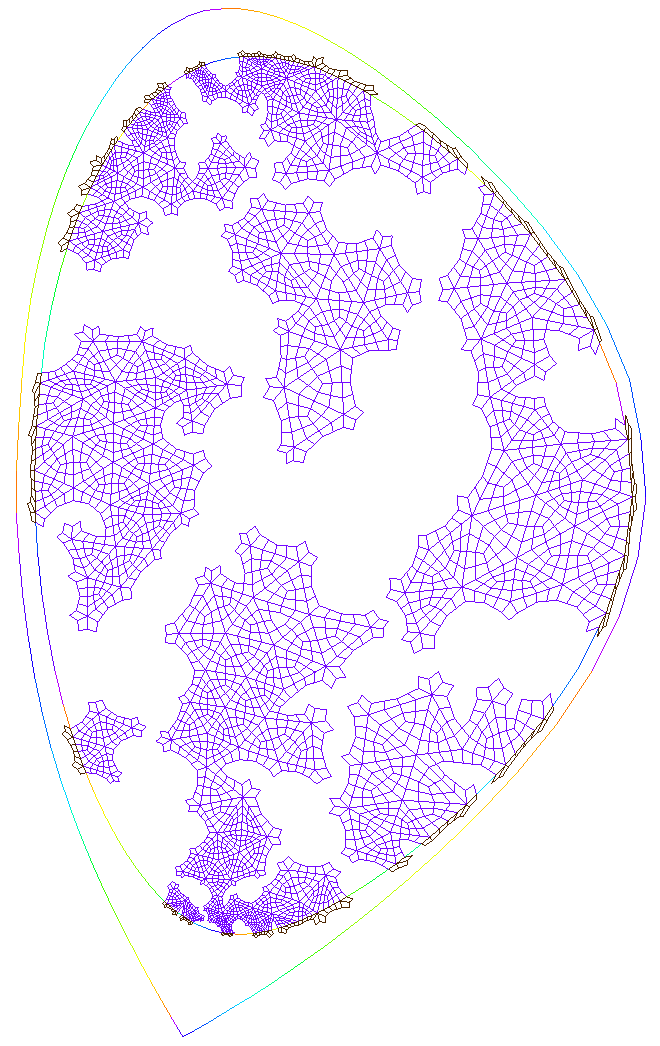
\includegraphics[scale=.5]{images/tokamak_layer_mesh_adapt_fine_1_pre.pdf}}\quad
\subfigure[{rank = 2}\label{fig:tokamak_layer_mesh_adapt_fine_2_pre}]
{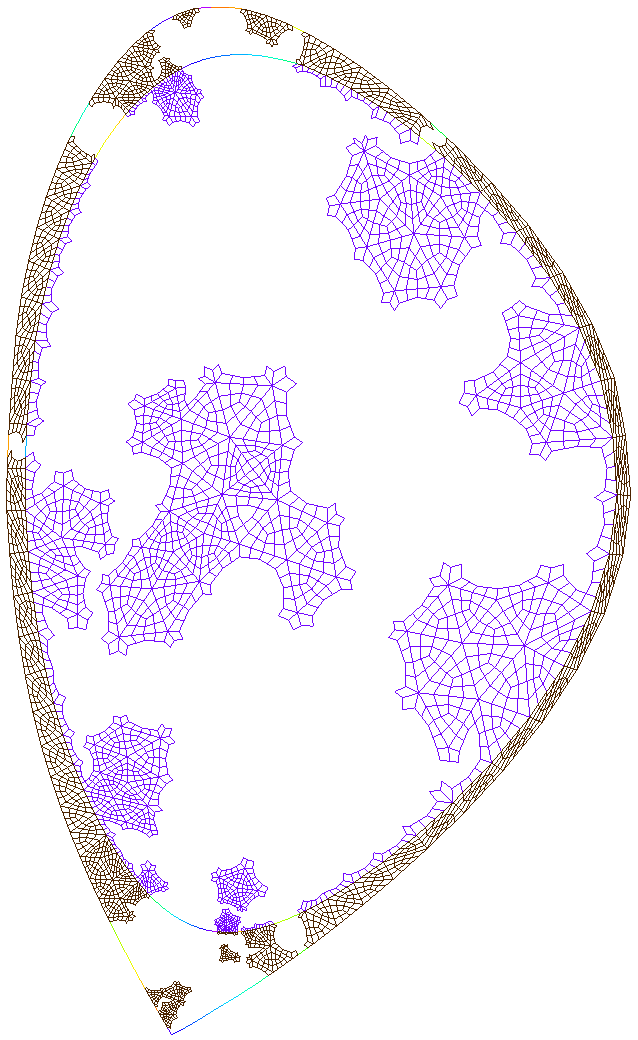
\includegraphics[scale=.5]{images/tokamak_layer_mesh_adapt_fine_2_pre.pdf}}\quad
\subfigure[{rank = 3}\label{fig:tokamak_layer_mesh_adapt_fine_3_pre}]
{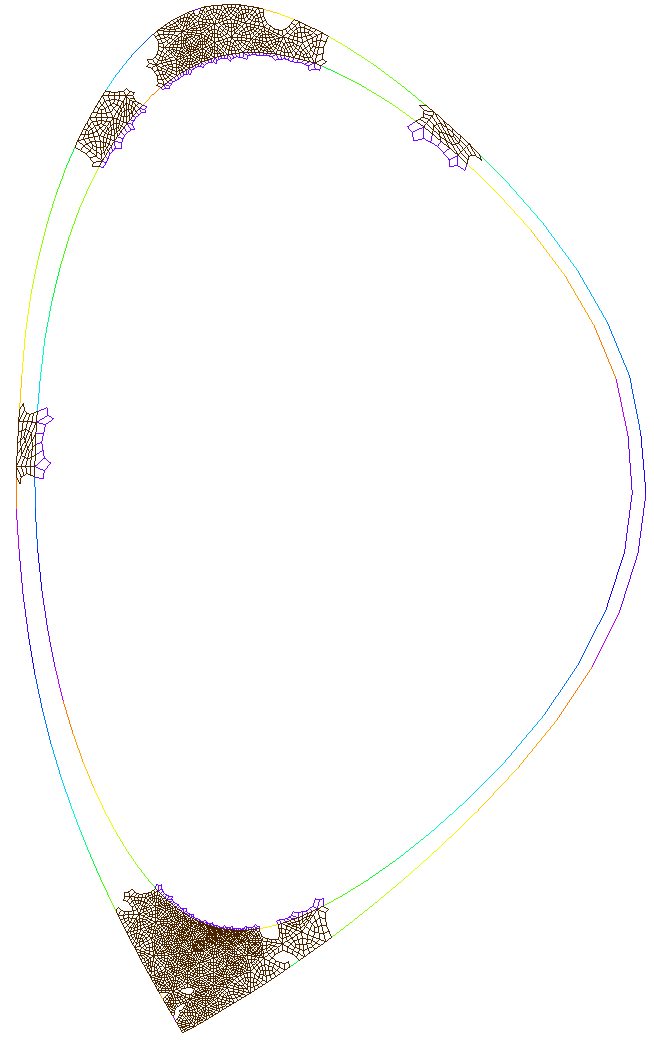
\includegraphics[scale=.5]{images/tokamak_layer_mesh_adapt_fine_3_pre.pdf}}\quad
\caption{Prepartitioning of a Tokamak section.}\label{fig:prepartitioning}
\end{figure}

\begin{figure}
\centering
\subfigure[{rank = 0}\label{fig:tokamak_layer_mesh_adapt_fine_0_par}]
{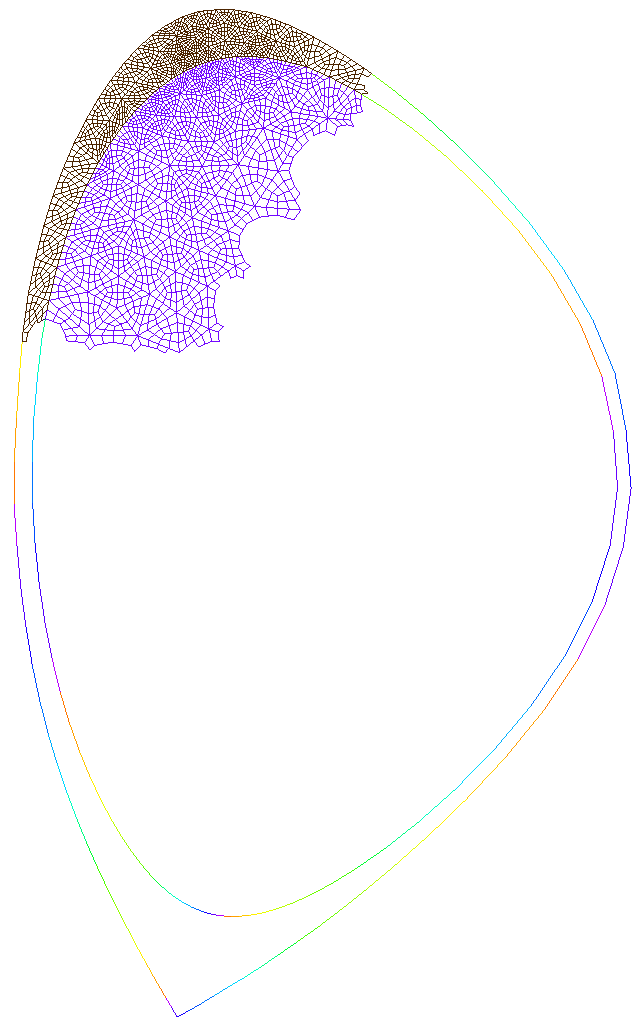
\includegraphics[scale=.5]{images/tokamak_layer_mesh_adapt_fine_0_par.pdf}}\quad
\subfigure[{rank = 1}\label{fig:tokamak_layer_mesh_adapt_fine_1_par}]
{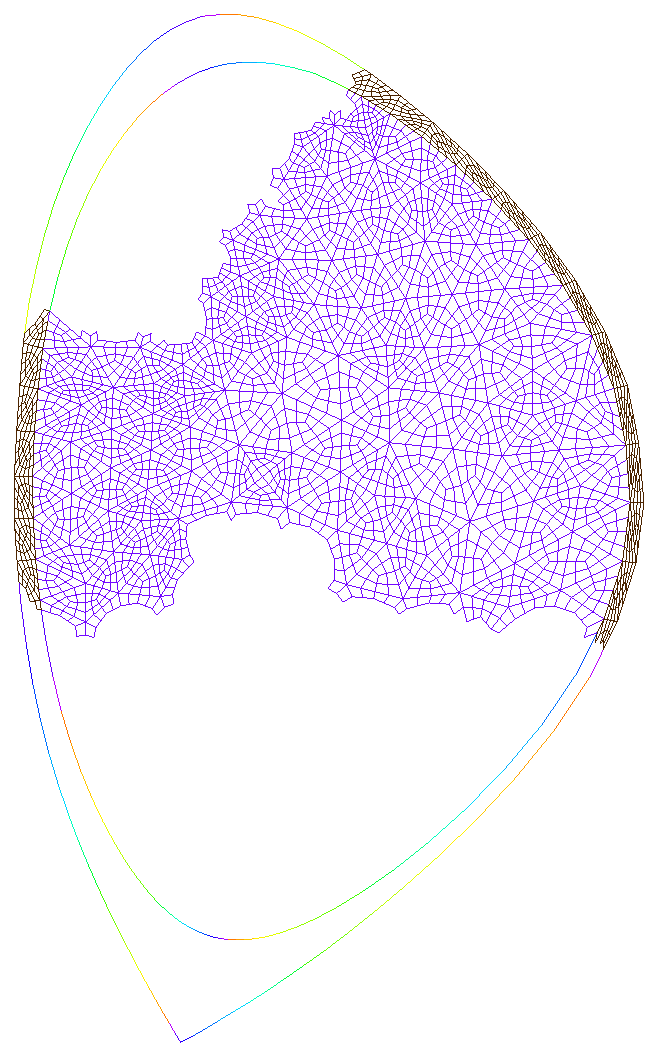
\includegraphics[scale=.5]{images/tokamak_layer_mesh_adapt_fine_1_par.pdf}}\quad
\subfigure[{rank = 2}\label{fig:tokamak_layer_mesh_adapt_fine_2_par}]
{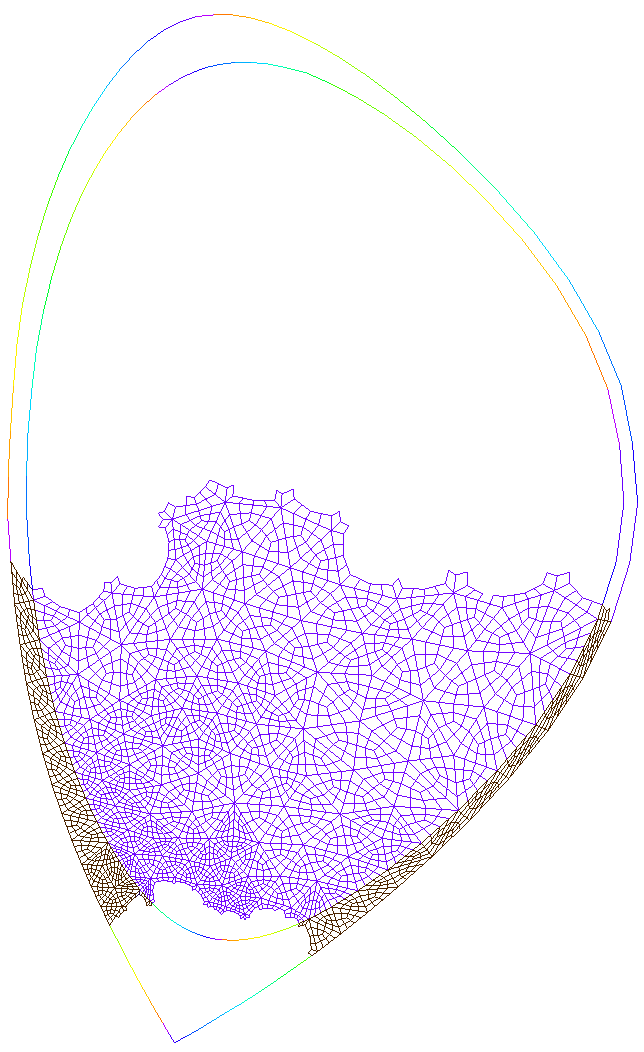
\includegraphics[scale=.5]{images/tokamak_layer_mesh_adapt_fine_2_par.pdf}}\quad
\subfigure[{rank = 3}\label{fig:tokamak_layer_mesh_adapt_fine_3_par}]
{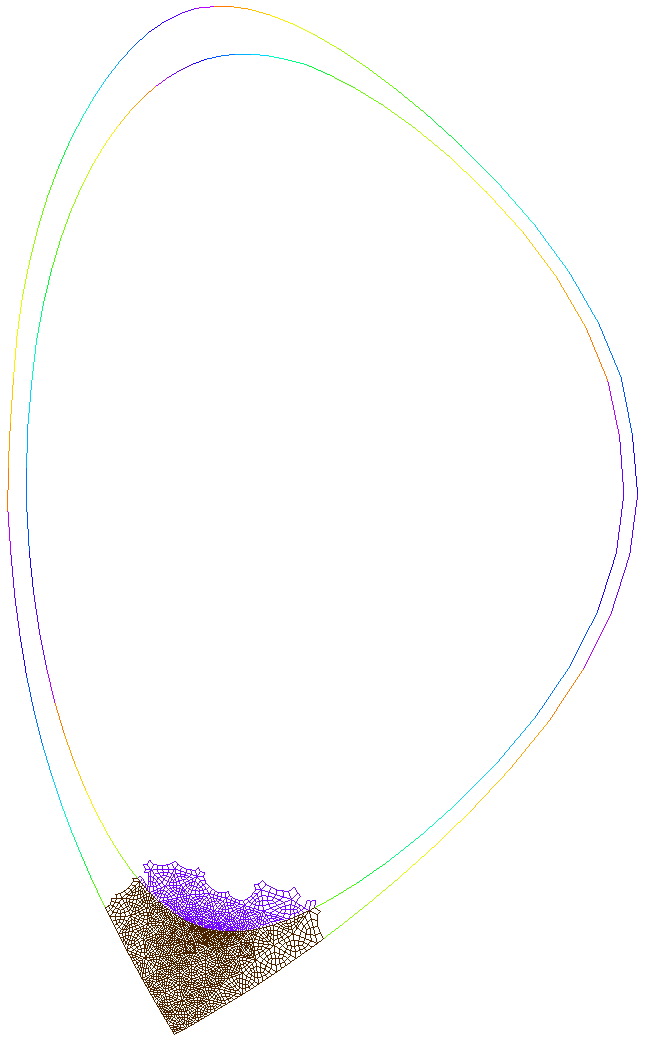
\includegraphics[scale=.5]{images/tokamak_layer_mesh_adapt_fine_3_par.pdf}}\quad
\caption{Partitioning of a Tokamak section.}\label{fig:partitioning}
\end{figure}

\begin{figure}
\centering
\subfigure[{rank = 0}\label{fig:tokamak_layer_mesh_adapt_fine_0_ref}]
{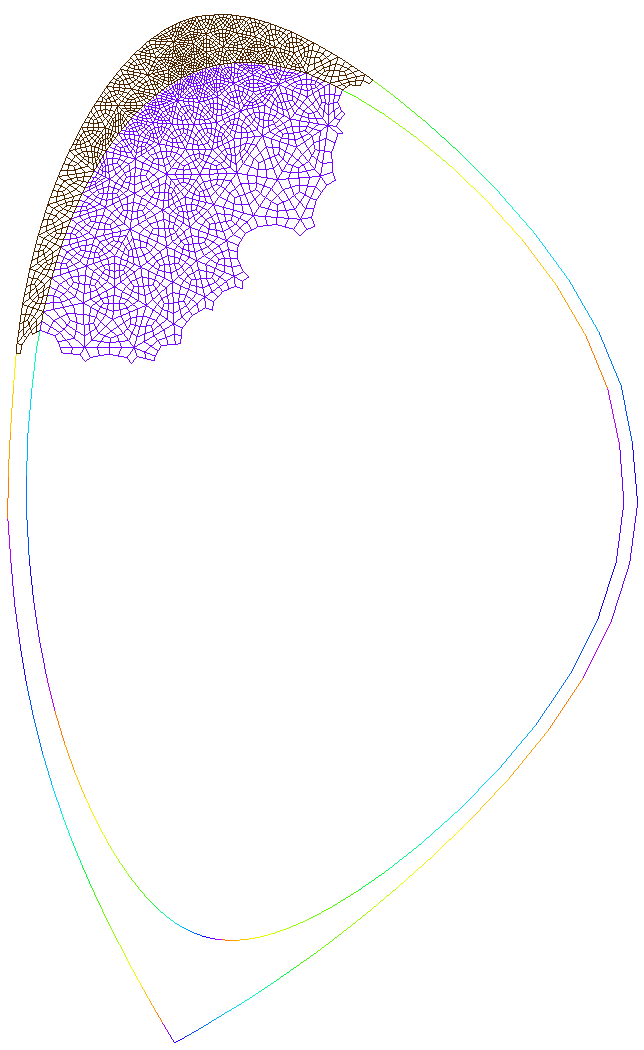
\includegraphics[scale=.5]{images/tokamak_layer_mesh_adapt_fine_0_ref.pdf}}\quad
\subfigure[{rank = 1}\label{fig:tokamak_layer_mesh_adapt_fine_1_ref}]
{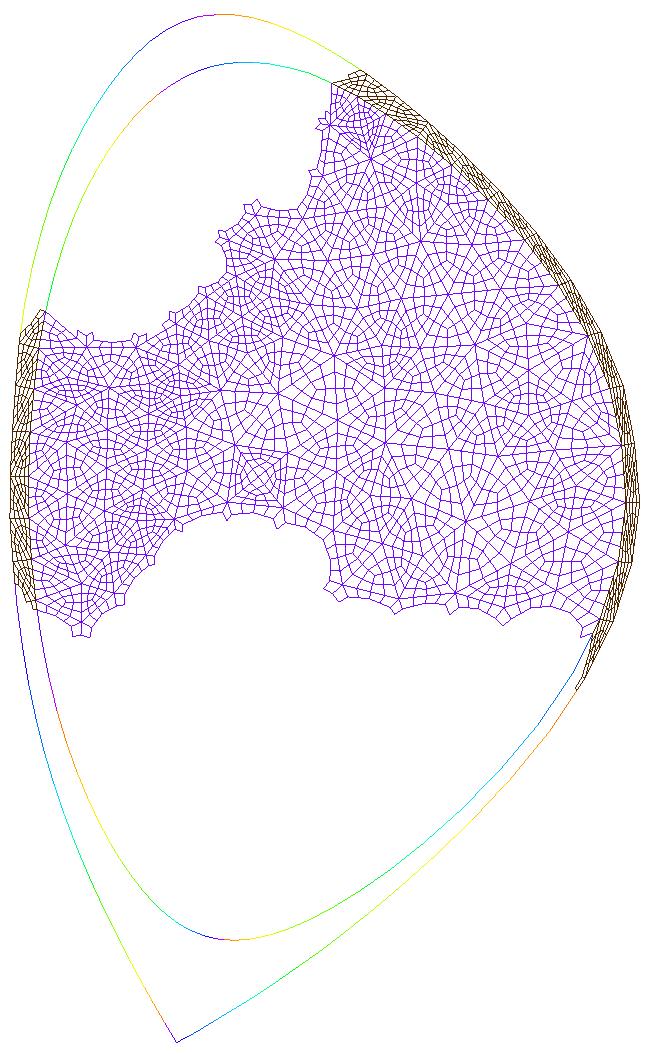
\includegraphics[scale=.5]{images/tokamak_layer_mesh_adapt_fine_1_ref.pdf}}\quad
\subfigure[{rank = 2}\label{fig:tokamak_layer_mesh_adapt_fine_2_ref}]
{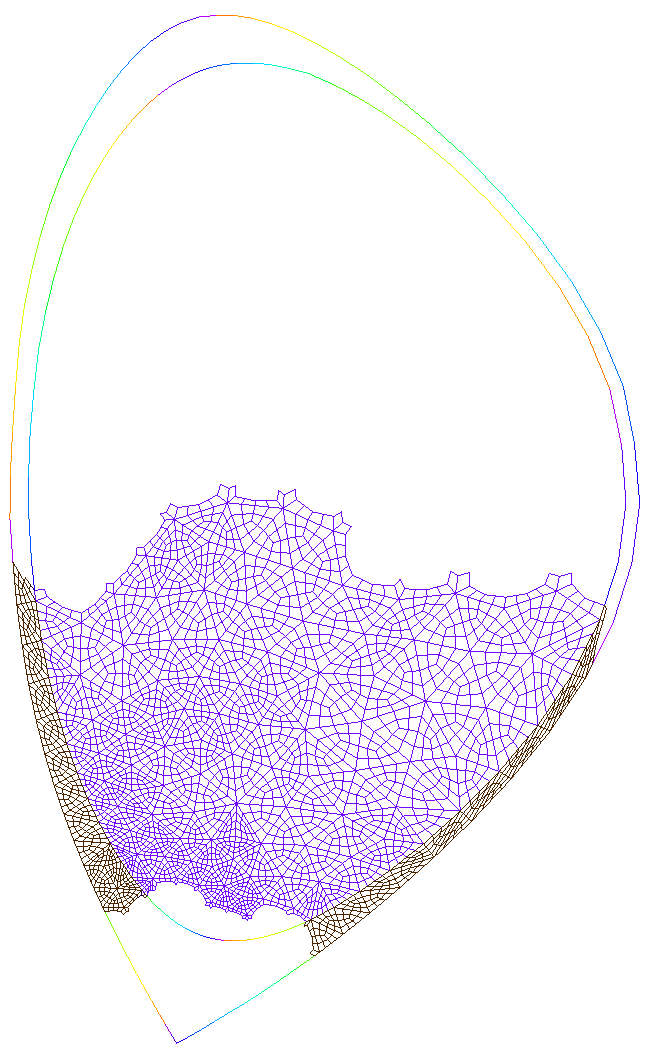
\includegraphics[scale=.5]{images/tokamak_layer_mesh_adapt_fine_2_ref.pdf}}\quad
\subfigure[{rank = 3}\label{fig:tokamak_layer_mesh_adapt_fine_3_ref}]
{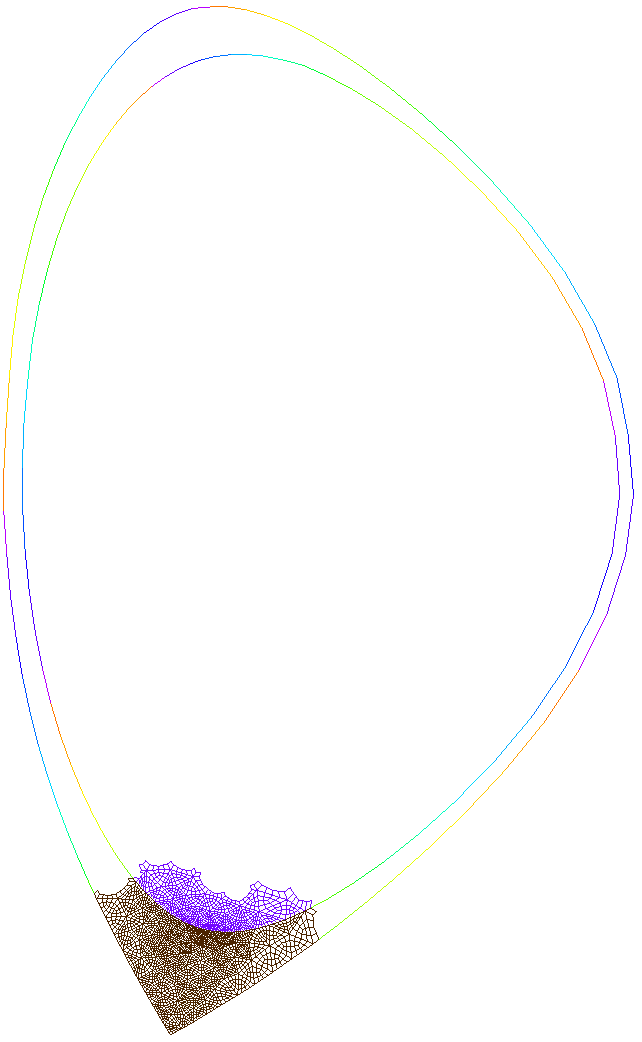
\includegraphics[scale=.5]{images/tokamak_layer_mesh_adapt_fine_3_ref.pdf}}\quad
\caption{5 refinements of a Tokamak section.}\label{fig:refinement}
\end{figure}
\newpage

\subsection{Mirror machine section}\label{subsection:mirror_machine}
In Fig.(\ref{fig:mirror}) we report the meshed section of the magnetic fields lines inside a mirror machine; this mesh is partitioned over 8 processes, indicated by different colors.

\begin{table}
\centering
\begin{tabular}{|c|c|c|}
\hline
 N. Refinements & Time (s) & N. Ghosts\\
\hline
 0 & 0.23 & 163\\
\hline
 1 &  0.28 & 155\\
\hline
 2 & 0.35 & 153\\
\hline
 3 & 0.42 & 153\\
\hline
 4 & 0.49 & 153\\
\hline
 5 & 0.55 & 153\\
\hline
\end{tabular}
\caption{Mirror machine ($3.6\cdot 10^{4}$ elements).}
\label{tab:mirror_36k}
\end{table}

We compare the performances, in terms of execution time and reduction of number of ghosts, of \verb|ParMETIS| refine algorithm. In Tab.(\ref{tab:mirror_36k}) we use a mesh of $3.6\cdot 10^{4}$ elements starting from 0 refinements until 5 refinements. We can notice that the average number of ghosts slightly reduces with the first two refinements and after it remains constant: the improvement is about 6\%, so the parallel communication is reduced of the same amount. It is worth to compare the time of execution with a larger grid. In fact, while in the small grid case the time of execution is influenced mainly by the reading and partitioning, then each refinement contributes by a fraction of the total time, in the second case (cmp. Tab.(\ref{tab:mirror_26M})) every refinement takes almost three times the time spent in the first part. This means that the complexity of the refinement algorithm is not linear. The final improvement after 5 refinements is 6.5\%.

\begin{table}
\centering
\begin{tabular}{|c|c|c|}
\hline
 N. Refinements & Time (s) & N. Ghosts\\
\hline
 0 & 63.43 & 1369\\
\hline
 1 &  242.23 & 1319\\
\hline
 2 & 418.63 & 1300\\
\hline
 3 & 604.96 & 1292\\
\hline
 4 & 778.94 & 1285\\
\hline
 5 & 956.44 & 1280\\
\hline
\end{tabular}
\caption{Mirror machine ($2.6\cdot 10^{6}$ elements).}
\label{tab:mirror_26M}
\end{table}

\begin{figure}
\centering
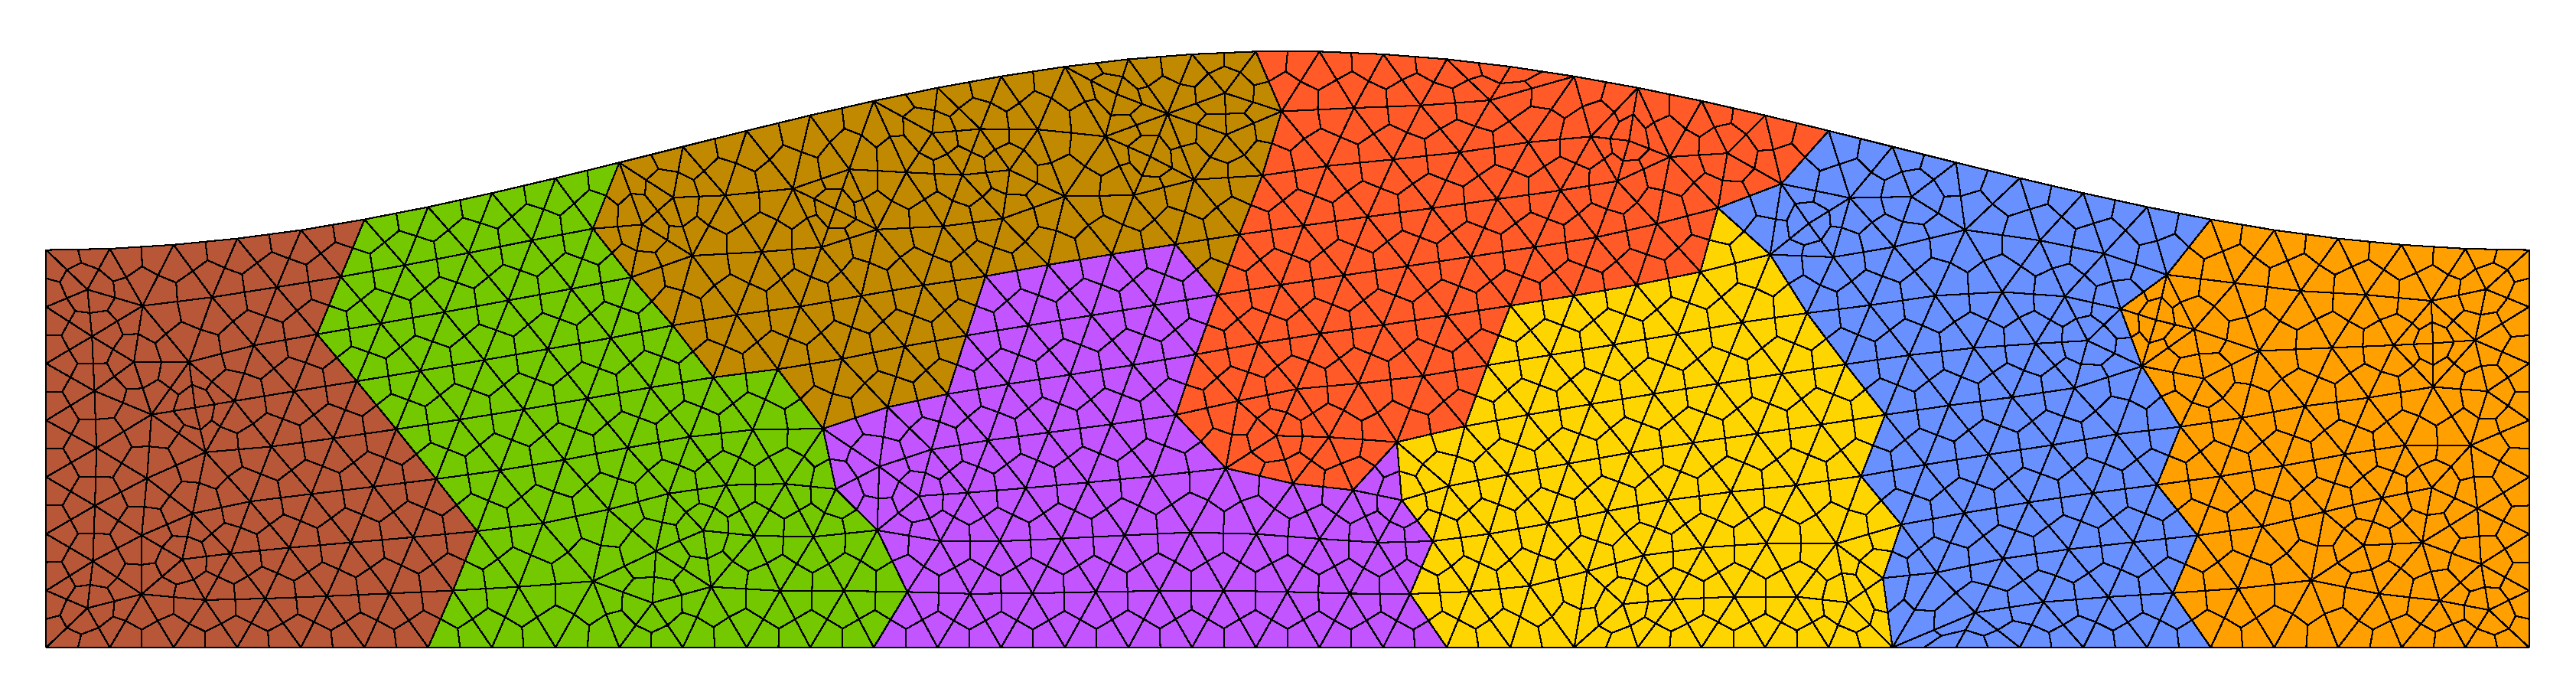
\includegraphics[scale=.27]{images/mirror_partitioned.eps}
\caption{Partitioning of a mirror machine section (2350 elements).}
\label{fig:mirror}
\end{figure}


\chapter{Simulator}\label{ch:simulator}
In this chapter we explain the core part of the code which is devoted to define the classes necessary to implement our discrete equations, the linear and the nonlinear solver and the storing of the solution. We will give a general overview of the main methods, the logic behind them and how all the classes are related.

We design our code to achieve a great flexibility since the final goal of the project is to obtain a framework for multi-physics simulations. For this reason we wrote a code strongly object-oriented with base classes very generic to permit a simple implementation of new basis, quadrature formulas, discrete equations, etc. . To achieve this results we used templates since they are statically bound and we tried to avoid virtual function, which are dynamically bound. Cmp. \cite{cpp_primer}.

In Fig.(\ref{fig:sem_diagram}) it is shown a simplified diagram of the main classes which will be explained in this chapter.

\begin{figure}
\centering
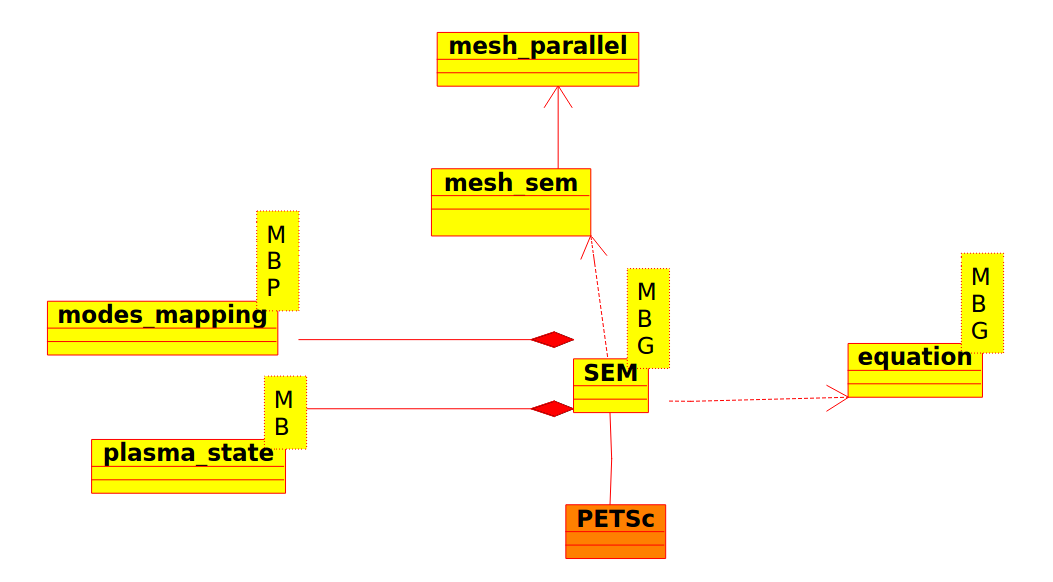
\includegraphics[scale=0.3]{images/sem_diagram.png}
\caption{Simulator: classes structure.}\label{fig:sem_diagram}
\end{figure}

\section{Mesh}\label{sec:mesh}
The mesh is defined in the class \verb|mesh_sem| which inherits from the class \verb|mesh_parallel|. The class \verb|mesh_parallel| already contains all the methods and all the informations needed by our method; the only additional information needed is the local degree of the basis. Therefore this derived class contains a vector where are stored all the elements degrees which are locally stored. Since we need also to know the degrees of each ghost we used the class \verb|ghost_communication| to keep updated these values. Moreover there are implemented some inline methods to extract the maximum degree, the local degree of an element and the degree of the edge which is the minimum degree of the two elements which share that edge.

\section{Polynomial basis}\label{sec:modal_basis}

We choose to adopt a modal basis which is built in a recursive way using the Legendre polynomials $\{L_k\}_0^p$ which are defined, over the logical domain $[-1,1]$, as
\begin{equation}
  \begin{cases}
    L_0(\hat{x})=1\\
    L_1(\hat{x})=\hat{x}\\
    (k+1)L_{k+1}(\hat{x})=(2k+1)\hat{x}L_k(\hat{x})-kL_{k-1}(\hat{x}),\quad k=1,\dots,p_m-1
  \end{cases}
\end{equation}
with derivatives
\begin{equation}
  (1-\hat{x}^2)L'_k(\hat{x})=kL_{k-1}(\hat{x})-k\hat{x} L_k(\hat{x}),\quad k\geq 1.
\end{equation}
These polynomials form a modal basis of $\mathbb{P}_p(-1,1)$, indeed it is hierarchic, which means that the expansion set of order $p$ is contained within the expansion set of order $p+1$. By definition they are orthogonal respect the Legendre inner product, $(u,v)_w=\int uvw$ with $w\equiv 1$ so it is the usual inner product in $L^2(-1,1)$.
\medskip

The Legendre polynomials are implemented in the class \verb|legendre| which contains four variables, stored as \verb|vector<vector<double> >|, to store the coefficients of the Legendre polynomials and their derivatives both in ascending and descending orders. The $i^{th}$-row store the coefficients of polynomials $L_i$. We store the coefficients in both order because sometimes it is necessary to pass this array of coefficients to some C library functions which operates with ascending or descending order array.

The main method are the ones which returns the vector of coefficients: \verb|c(j)|, \verb|c_der(j)|, \verb|c_reverse(j)| and \verb|c_der_reverse(j)| where \verb|j| is the number of the polynomials. If \verb|j| is bigger than the maximum value stored, the new coefficients are evaluated and added to the vectors, before returning the reference.
\medskip

Unfortunately the Legendre modal basis cannot be extended, without great difficulties, to an elemental decomposition which is globally $C^0$ therefore we adopt a new defined using the Legendre polynomials. We defined our basis with the following recursive formula
\begin{equation}\label{eq:modal_basis_1D}
  \begin{cases}
    \phi_0(\hat{x})=\frac{1-\hat{x}}{2}\\
    \phi_1(\hat{x})=\frac{1+\hat{x}}{2}\\
    \phi_k(\hat{x})=\frac{1}{\sqrt{2(2k-1)}}(L_{k-2}(\hat{x})-L_k(\hat{x})), & k=2,\dots,p
  \end{cases}
\end{equation}
which defines a modal hierarchic boundary-adapted basis.

\begin{figure}
\centering
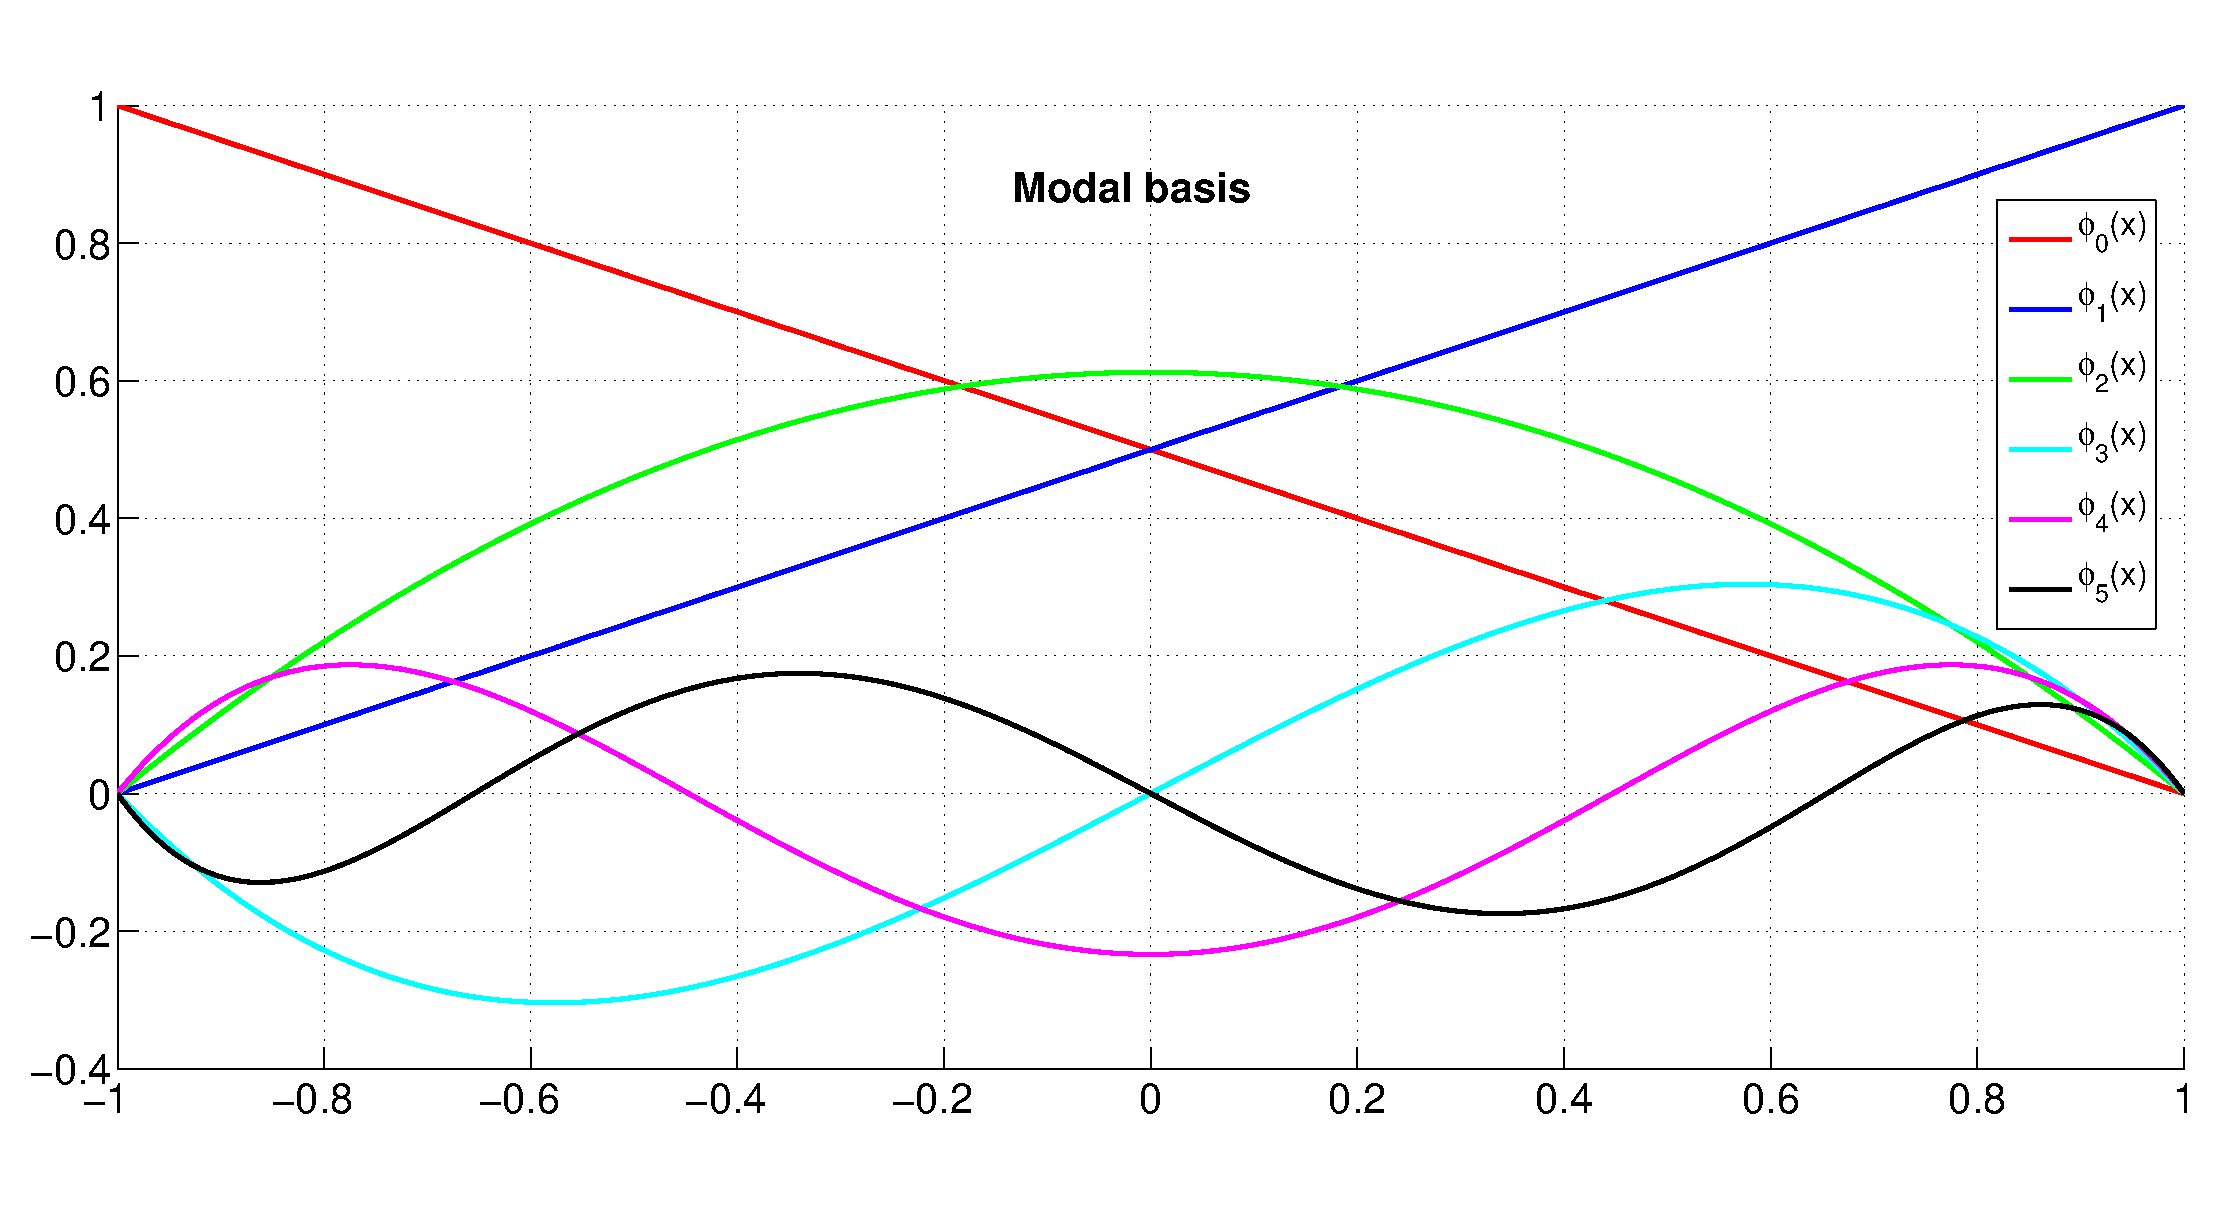
\includegraphics[scale=0.3]{images/1D_basis.eps}
\caption{Modal basis $\phi_i(\hat{x})$, with $i\in\{0,\dots,5\}$, defined on the interval [-1,1].}\label{fig:1D_basis}
\end{figure}

The first six modes are plotted in Fig.(\ref{fig:1D_basis}). A hierarchic basis is convenient, from a computational point of view, to increase locally the degree of polynomials which is necessary when one needs to perform a p-refinement. Indeed, for a hierarchic basis, it holds that the basis of $\mathbb{P}_p$ is a subset of $\mathbb{P}_{p+1}$ therefore
\begin{equation}
  \{\phi_i\}_0^p\subset\{\phi_i\}_0^{p+1}=\{\phi_i\}_0^p\cup\{\phi_p+1\}.
\end{equation}

A basis of $\mathbb{P}_p(-1,1)$ is defined boundary-adapted if contains two modes, called \textit{vertex functions}, that are nonzero at precisely one endpoint of the interval (red and blue functions plotted in Fig.(\ref{fig:1D_basis})), and $p-1$ modes, called \textit{bubble functions}, that vanish at both endpoints (green, light blue, magenta and black functions plotted in Fig.(\ref{fig:1D_basis})). The drawback of the new basis is that it is not orthogonal.
\medskip

It is possible to demonstrate that the derivatives of our basis can be evaluated using the following iterative formula
\begin{equation}
  \begin{cases}
    \phi'_0(\hat{x})=-\frac{1}{2}\\
    \phi'_1(\hat{x})=\frac{1}{2}\\
    \phi'_k(\hat{x})=-\sqrt{\frac{2k-1}{2}}L_{k-1}(\hat{x}), & k=2,\dots,p.
  \end{cases}
\end{equation}
\medskip

We implement a base class, called \verb|basis_function|, which is a pure abstract class for basis management. It contains two matrices, type \verb|vector<vector<double> >|, to store the coefficients of the basis and the coefficients of its derivatives in descending order. It has two methods to evaluate the value of the basis and the value of its derivative in a certain point of the logical domain, respectively \verb|eval(x,j)| and \verb|eval_der(x,j)|. It has a pure abstract method, \verb|set_basis_order(j)|, which must be overload; it fills the vector of coefficients of the basis. Before using the methods to evaluate the basis or its derivative in a certain points it is necessary to call once the method \verb| set_order(j)|. This method call the overloaded method \verb|set_basis_order| to fill the vector with the coefficients of the basis and than it computes and stores the coefficients of the derivatives of the basis in another vector.
\medskip

Our basis is implemented in the class \verb|leg_modal_basis| which inherits from the pure abstract class \verb|basis_function|. It simply has a variable of type \verb|legendre| and the method \verb|set_basis_order| which is the implementation of the recursive formula to evaluate the basis Eq.(\ref{eq:modal_basis_1D}).
\medskip

From the one-dimensional basis we can build the two-dimensional basis. Let's start defining on the logical element, the square $\hat{\Omega}=[-1,1]\times[-1,1]$, the space of polynomials of degree $\leq N$ in each coordinate $\mathbb{Q}_N$, for $N\geq 1$. We cannot have different maximum degrees on the two space variables because it is integral to definition of $\mathbb{Q}_N$. More precisely $\mathbb{Q}_N$ is defined as
\begin{equation}
  \mathbb{Q}_N(\hat{\Omega})=\mathrm{span}\{\hat{x}^i \hat{y}^j, \: 0\leq i,j\leq N,(\hat{x},\hat{y})\in \hat{\Omega}\}
\end{equation}
and its dimension is $(N+1)^2$.

For that space $\mathbb{Q}_N(\hat{\Omega})$ we choose to adopt a boundary-adapted modal basis. The basis is simply constructed using the tensor product of one-dimensional basis; the resulting functions are defined on Cartesian products of intervals. Precisely, given two families$\{\phi_i(\hat{x})\}_0^p$ and $\{\phi_j(\hat{y})\}_0^p$ with $0\leq i,j\leq N$, the family $\{\phi_{ij}(\hat{x},\hat{y})\}_0^p$ is defined as
\begin{equation}
  \phi_{ij}(\hat{x},\hat{y})=\phi_i(\hat{x})\phi_j(\hat{y}),\qquad i,j=0,\dots,N
\end{equation}
In Fig.(\ref{fig:2D_basis}) is shown the basis in the special case of $p=2$.

\begin{figure}
\centering
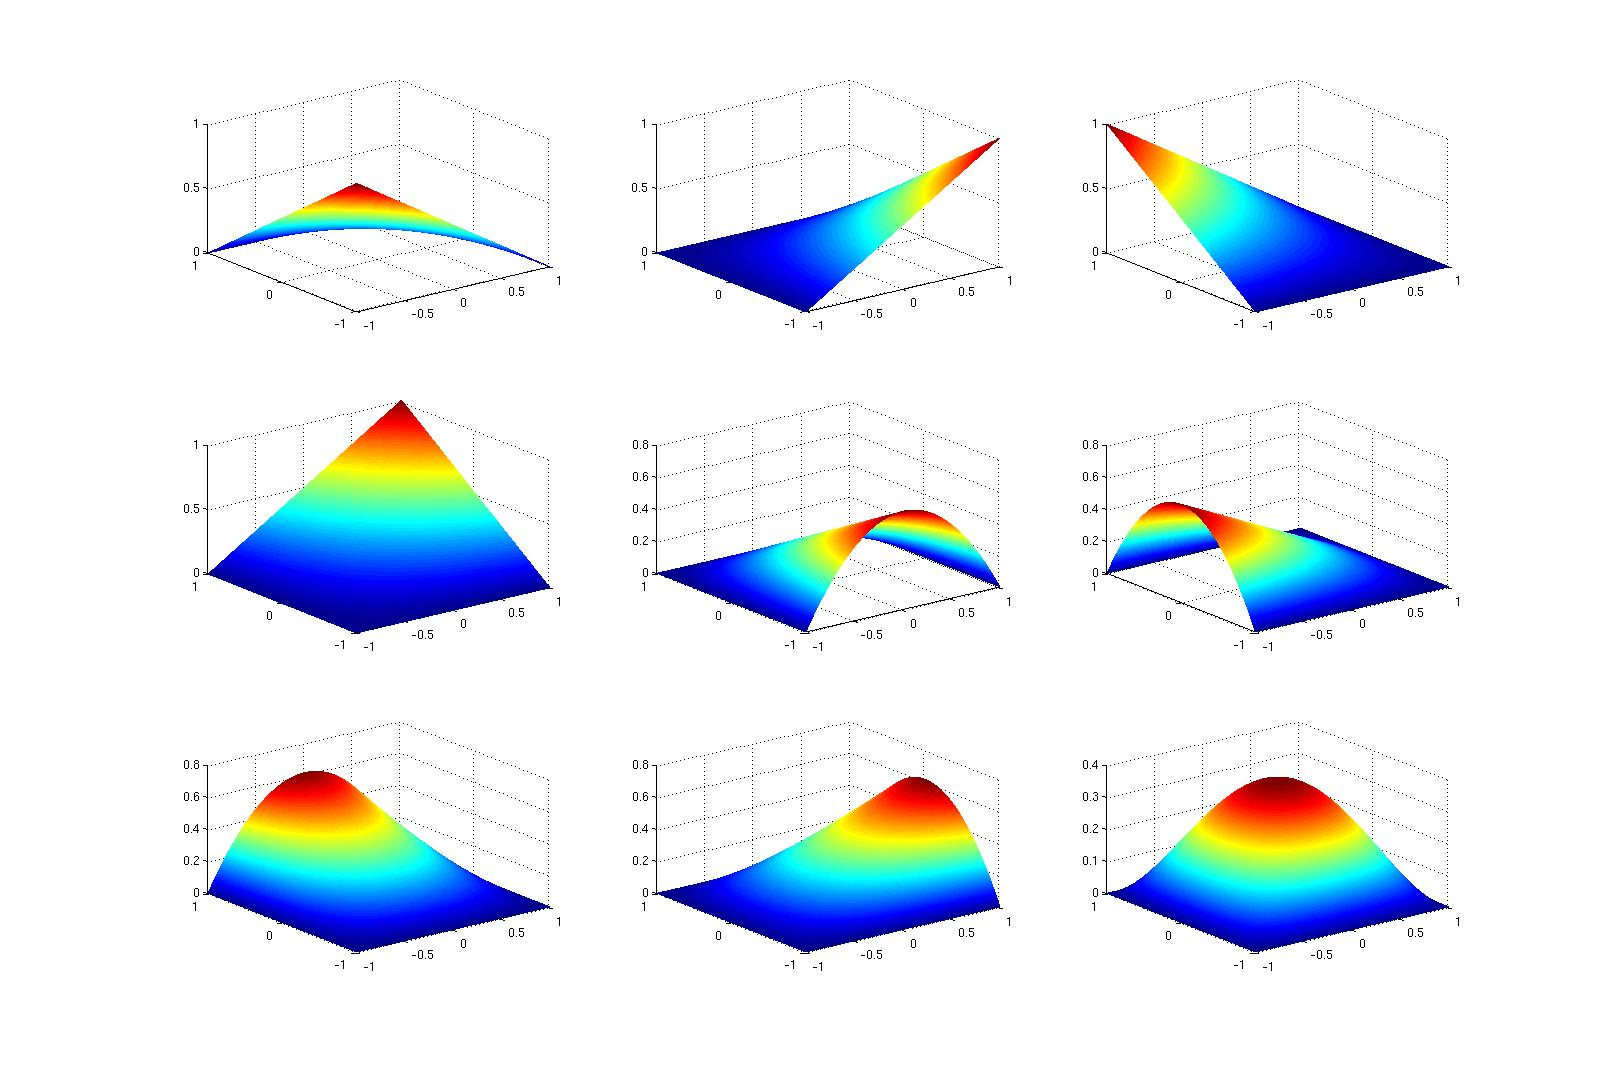
\includegraphics[scale=0.25]{images/2D_basis.jpg}
\caption{Modal basis $\phi_i(\hat{x})\phi_j(\hat{y})$, with $i,j\in\{0,\dots,2\}$, defined on the logical domain $[-1,1]\times[-1,1]$.}\label{fig:2D_basis}
\end{figure}

The usage of a modal basis corresponds to projection operator of $\psi$ over the space $\mathbb{Q}_N$.
\medskip

Any boundary-adapted basis is formed by three different type of modes:
\begin{itemize}
  \item $(N-1)^2$ \textit{bubble functions}, $(i\geq 2)\wedge(j\geq 2)$, which vanish on the boundary $\partial\hat{\Omega}$;
  \item 4 \textit{vertex functions}, $(i\leq 1)\wedge(j\leq 1)$, which do not vanish at precisely one vertex;
  \item $4(N-1)$ \textit{edge functions}, $\big((i\leq 1)\wedge(j\geq 2)\big)\vee\big((i\geq 2)\wedge(j\leq 1)\big)$ which do not vanish at precisely one edge.
\end{itemize}

In Fig.(\ref{fig:2D_basis}), starting from the top on the left and going to the bottom of the right, we have the 4 vertex functions, then 4 edge functions and last the unique bubble function which form the modal basis in the special case of $p=2$. Instead, Fig.(\ref{fig:modes_diagram}) is a diagram which shows where the modes are different from zero. Therefore we can see each vertex function to which vertex of the logical domain refers, each edge function to which edge of the logical domain refers and finally the bubble functions in the center of the domain since they vanish on the border.

\begin{figure}
\centering
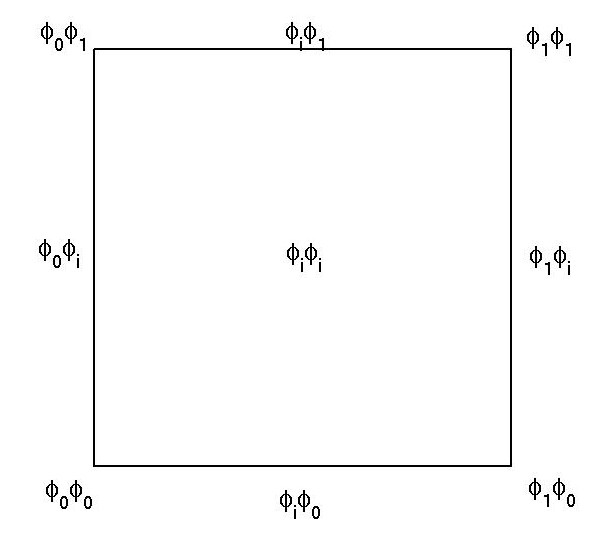
\includegraphics[scale=0.25]{images/modes_diagram.jpg}
\caption{Diagram of the modes, $i\geq 2$.}\label{fig:modes_diagram}
\end{figure}

The quadrilateral basis is therefore defined as:
\begin{description}
 \item[vertex]
   \begin{equation}
      \begin{cases}
	\phi_0(\hat{x})\phi_1(\hat{y})=\frac{1-\hat{x}}{2}\frac{1+\hat{y}}{2}\\
	\phi_1(\hat{x})\phi_1(\hat{y})=\frac{1+\hat{x}}{2}\frac{1+\hat{y}}{2}\\
	\phi_1(\hat{x})\phi_0(\hat{y})=\frac{1+\hat{x}}{2}\frac{1-\hat{y}}{2}\\
	\phi_0(\hat{x})\phi_0(\hat{y})=\frac{1-\hat{x}}{2}\frac{1-\hat{y}}{2}
      \end{cases}
   \end{equation}
  \item[edge]
    \begin{equation}
	\begin{cases}
	  \phi_i(\hat{x})\phi_1(\hat{y})=\frac{\sqrt{2(2i-1)}}{i}\frac{1-\hat{x}}{2}\frac{1+\hat{x}}{2}P^{1,1}_{i-2}(\hat{x})\frac{1+\hat{y}}{2}\\
	  \phi_1(\hat{x})\phi_i(\hat{y})=\frac{1+\hat{x}}{2}\frac{\sqrt{2(2j-1)}}{j}\frac{1-\hat{y}}{2}\frac{1+\hat{y}}{2}P^{1,1}_{j-2}(\hat{y})\\
	  \phi_i(\hat{x})\phi_0(\hat{y})=\frac{\sqrt{2(2i-1)}}{i}\frac{1-\hat{x}}{2}\frac{1+\hat{x}}{2}P^{1,1}_{i-2}(\hat{x})\frac{1-\hat{y}}{2}\\
	  \phi_0(\hat{x})\phi_i(\hat{y})=\frac{1-\hat{x}}{2}\frac{\sqrt{2(2j-1)}}{j}\frac{1-\hat{y}}{2}\frac{1+\hat{y}}{2}P^{1,1}_{j-2}(\hat{y})
	\end{cases}
    \end{equation}
  \item[interior]
    \begin{equation}
      \phi_i(\hat{x})\phi_j(\hat{y})=\frac{\sqrt{2(2i-1)}}{i}\frac{1-\hat{x}}{2}\frac{1+\hat{x}}{2}P^{1,1}_{i-2}(\hat{x})\frac{\sqrt{2(2j-1)}}{j}\frac{1-\hat{y}}{2}\frac{1+\hat{y}}{2}P^{1,1}_{j-2}(\hat{y})
    \end{equation}
\end{description}
where $P^{\alpha,\beta}_k(\hat{x})$ is the $k$-th order Jacobi polynomial and $i,j\geq 2$.
\medskip

We want to point out that, to have a lighter notation, we dropped the $\:\hat{}\:$ over the function $\phi$ since it is obvious that they are defined over the logical domain. Since it is possible to find an univocal mapping $(i,j)\longrightarrow i'$ which maps the numbering of the modes, in Ch.(\ref{chapter:sem}) we didn't explicitly write the basis like a tensor product but simply as $\hat{\phi}_{i'}(\mathbf{\hat{x}})$.

\section{Gaussian integration}\label{sec:gaussian_integration}
In order to evaluate the inner products of the discrete variational formulation, we choose the Gauss-Legendre-Lobatto (GLL) formula which is a Gaussian quadrature formula which has two nodes at the boundary on the interval. The $N+1$ GLL nodes $\{\hat{x}_n\}_0^N$ for the interval $[-1,1]$ are the endpoints of interval, to ensure the continuity between elements, and the maxims and minims of the $N$-th degree Legendre polynomial therefore the roots of the first derivative of $L_N$ while the weights are defined as
\begin{equation}
  w_n=\frac{2}{N(N+1)}\frac{1}{L^2_N(\hat{x}_n)}.
\end{equation}
Its degree of precision is $2N-1$ which implies that the discrete inner product is equal to the classical inner product if the product of the two function belongs to $\mathbb{P}_{2N-1}$.
\medskip

The GLL nodes and weights are evaluated using the class \verb|gaussian_integration| which contains two matrices, type \verb|vector<vector<double> >|, where are stored the nodes and the weights and a variable of type \verb|legendre| which is used to evaluate the Legendre polynomials. The zeros of the $L'_N$ are evaluated numerically using the function \verb|gsl_poly_complex_solve| of the library \verb|GSL| which accept an array of coefficients and return the zeros of the polynomials. Moreover there are some inline methods which returns, given the order of the polynomial to integrate, the necessary number of nodes to obtain an exact integration.

The methods \verb|get_nodes(j)| and \verb|get_weights(j)| return the reference to the \verb|j|-th row.
\medskip

Like for the modal basis, the GLL nodes and weights for the logical domain $\hat{\Omega}=[-1,1]\times[-1 1]$ are obtained taking the tensor product of the one-dimensional nodes and weights.

\section{Definition of the equations}
In Fig.(\ref{fig:equation_diagram}) it is reported the diagram which shows the structure of the classes involved in the definition of the equations.

\begin{figure}
\centering
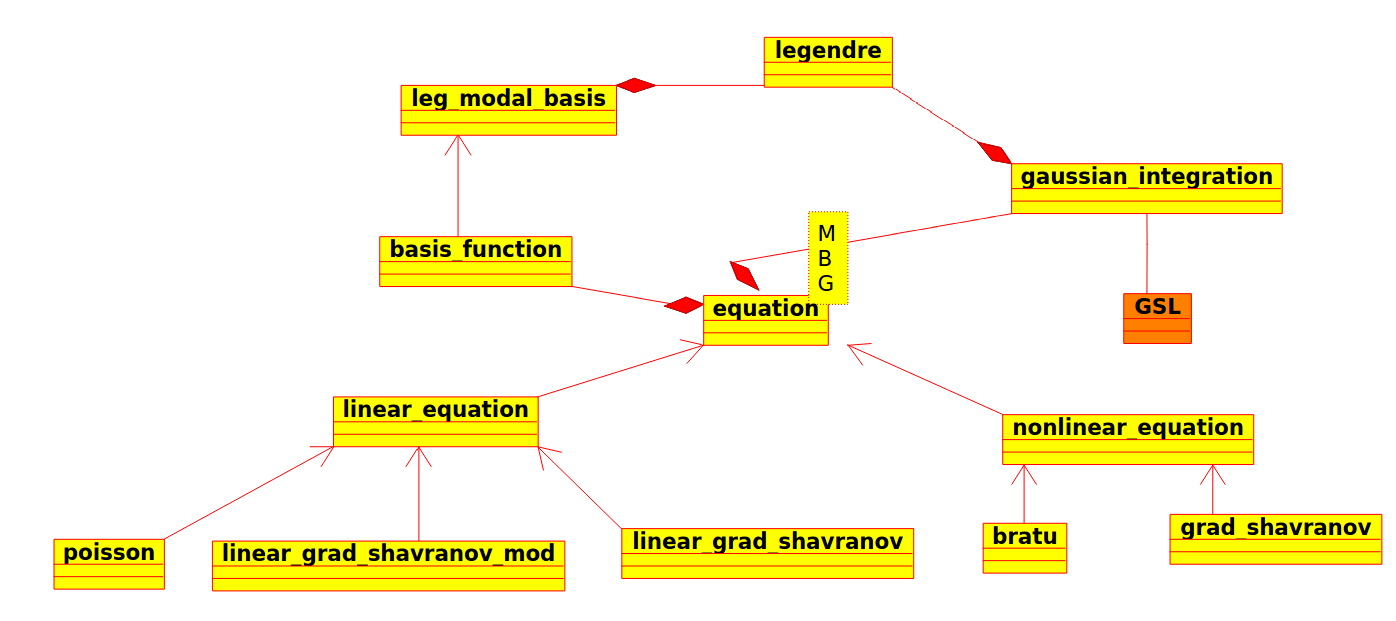
\includegraphics[scale=0.3]{images/equation_diagram.png}
\caption{Equation: classes structure.}\label{fig:equation_diagram}
\end{figure}

The base class is \verb|equation|; its constructor takes like arguments only a pointer to the mesh. It has two protected templated variables for the basis and for the numerical integration. When the constructor is called it extracts from the mesh the maximum degree of the basis needed. After that it constructs the basis variable according to that degree and it also constructs the numerical integration variable with the necessary number of points to obtain an exact polynomial integration up to that degree. Since the modes and their first derivatives will be evaluated in the same quadrature points a lot of time, these values are stored in a three-dimensional matrix where the first dimension is the mode number, the second is the number of quadrature points desired and the third the values of the mode in the nodes. The same matrix is evaluated for the first derivatives. These matrices are filled using the method \verb|compute_basis|.

Another method called automatically in the constructor is \verb|compute_dirichlet_coeff|, which, for each boundary lines, computes the coefficients of the projection of the Dirichlet condition over the basis. These projection coefficients are stored in a private variable of type \verb|vector<vector<double> >|.
\medskip

The class \verb|linear_equation| and \verb|nonlinear_equation| inherit from this base class. They are very similar since they implements the routines used to evaluate the contribution of the stiffness matrix and the RHS.

The class for the linear equations have three pure virtual methods \verb|eval_LHS|, \verb|eval_RHS| and \verb|eval_neumann| which must be overload in the derived classes. In these methods there must be written the parts of the discrete formulation inside the summations. This methods are used by \verb|LHS|, \verb|RHS| and \verb|neumann| which evaluate the Jacobian of the transformations and loop over the elements and the quadrature nodes. These are the methods used to evaluate the contribution inside the stiffness matrix and the right hand term of the final linear system.

Similarly, the class \verb|non_linearequation| has the methods \verb|LHS|, \verb|RHS| and \verb|neumann| but now they have a different meaning since the LHS for the non linear equation is the Jacobian of the Newton abstract methods while the RHS is the functional of the method multiplied by $-1$ . The method which must be overload are called \verb|eval_Jacobian|, \verb|eval_F0| and \verb|eval_neumann|.
\medskip

We have implemented several different equations deriving their classes from the previous two in accordance to the nature of the equation. In Sec.(\ref{sec:exemples}) we describe each equations which we have implemented.

\section{Global operation}\label{sec:global_assembling}
To construct a globally $C^0$ continuous expansion from elemental contributions, we must match the local boundary modes with a similar shape: vertex and edge modes. Therefore we need to assemble the global system from the local systems creating a map between the global system and the local systems. The definition of this mapping is central to the global assembly process. If two neighboring elements have different local degree  a functional incompatibility between adjacent elements is created because of the continuity constraint which states that we have to match up all boundary modes. The solution is zeroing the coefficients of hanging degrees of freedom.
\medskip

Moreover it is important to notice that two edges modes must be glued together with the right sign when the degree of the modes is odd since the relative reference frame can be different. This fact is well shown in Fig.(\ref{fig:basis_assembling}) where there are represented two different situations which can happen when ones tries to glue together two edge modes of order 3. In the first case the two references frame are oriented in such a way that the modes has the same shape therefore no further operation is needed. Instead in the second case the two modes are reversed therefore it is necessary to subtract the modes instead of add them. We choose to adopt the convention that the leading reference frame is the one of the element with lower global index and the mode of the other element is glued according this conventional reference frame.

\begin{figure}
\centering
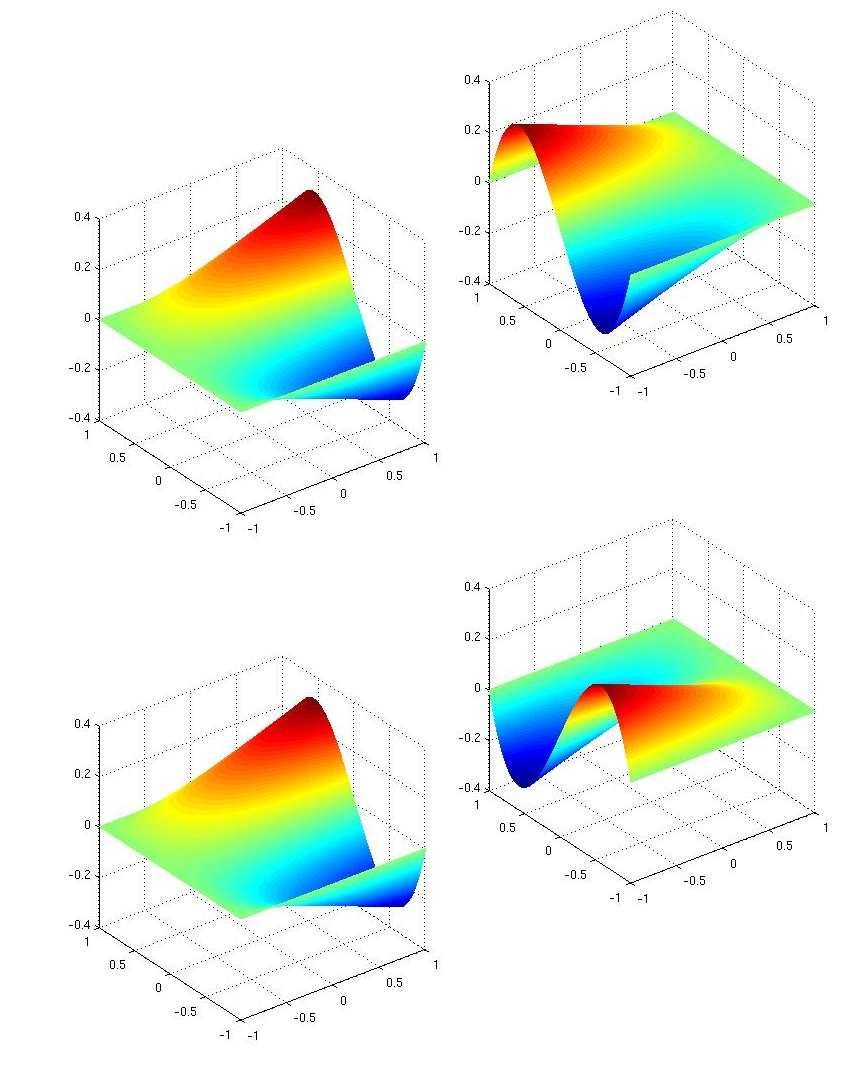
\includegraphics[scale=0.25]{images/basis_assembling_mod.jpg}
\caption{Global assembling for the edge mode $\phi_3(\hat{x})\phi_0(\hat{y})$ with two different local reference frames.}\label{fig:basis_assembling}
\end{figure}

The mapping which leads to a $C^0$ global basis is implemented in the class \verb|modes_mapping|. The constructor of the class calls the method \verb|create_mapping| which create the mapping. We number the modes following this order
\begin{itemize}
  \item vertex modes which are not degree of freedom;
  \item edge modes which are not degree of freedom;
  \item vertex modes which are degree of freedom;
  \item edge modes which are degree of freedom;
  \item bubble modes.
\end{itemize}
Therefore from the global number of the mode is straightforward to understand its type. This helps a lot during the stiffness assembling process.
\medskip

The map of the nodes is simply stored in a vector which has as many elements as the total number of the nodes; this vector is equal in each process. The map of the edge modes and bubble modes is stored in a matrix; each row represent one local element and has five entries. Each entry is the starting index of the modes corresponding to the first, second, third and fourth edge, with the convention adopted in Sec.(\ref{section:mono_cpu}). The fifth entry is the starting index of the bubble modes. The other global indices can be obtained from this matrix just adding the local numbering of the modes. For example if the mode $\phi_2\phi_0$, which is an edge mode, has global index $i$, the mode $\phi_5\phi_0$, which is an edge mode on the same edge, has global index $i+3$ since is the third mode of that edge.
\medskip

Other two important methods of the class are \verb|u(i,ii,e)|, which returns the coefficient of the solution referred to the modes $(\phi_i\phi_{ii})^e$, and \verb|u_sol(x,y,e)|, which returns $\hat{\psi}^e_{\delta}(\hat{x},\hat{y})$

\section{SEM simulator}
The part of the code devoted to the assembling of the linear system and the solution of it is implemented in the class \verb|SEM|. The constructor needs a pointer to the mesh, a pointer to the equation and a flag which can be \verb|STATIC_CONDENSATION_OFF|, default,  or \verb|STATIC_CONDENSATION_ON|. The constructor firstly creates the class \verb|mapping| and than create the necessary \verb|PETSc| variables calling the method \verb|create_petsc_variables|. The variables created depend on the type of the equation and on the flag:
\begin{itemize}
  \item linear equation without static condensation, created the matrix \verb|Abb| and the vectors \verb|Xb| and \verb|Fb|;
  \item linear equation with static condensation, created the matrices \verb|Abb|, \verb|Abi| and \verb|Abi| and the vectors \verb|Xb|, \verb|Xi|, \verb|Fb| and \verb|Fi|;
  \item nonlinear equation without static condensation, like the linear case without static condensation but in addition created the vector\verb|Xb_sol|;
  \item nonlinear equation with static condensation, like the linear with static condensation case but in addition created the vectors \verb|Xb_sol|, \verb|Xi_sol|.
\end{itemize}
All the matrices are of type \verb|MATMPIAIJ|, parallel sparse matrix, and all the vectors are of type \verb|VECMPI|, parallel vector.
\medskip

After the creation of the variables, the method \verb|create_scatter()|, using the \verb|PETSc| function \verb| VecScatterCreateToAll|, creates a scatter from the solution vector, which is parallel, to a sequential vector. This is necessary to retrieve the coefficients of the solution which are not locally stored. The solution vector for the linear case is \verb|Xb| (also \verb|Xi| with static condensation) while for the nonlinear case is \verb|Xb_sol| (also \verb|Xi_sol| with static condensation).
\medskip

The following step is the assembling of the matrix/matrices and of the vectors; to do this it is necessary the map created in the class \verb|modes_mapping| to put each contribution, evaluated through the class derived from \verb|equation|, in the right place. It is important to point out that the geometrically partition is not respected by the assembling process therefore a little more communication than necessary is carried out during this phase. Create a mapping which respects the geometric partition takes a lot more time than the one we created; for this reason we have chosen to do not respect the partition to speed up the code. The Dirichlet condition are imposed using the zeroing technique.
\medskip

Once that all the vectors and matrices are created, if the static condensation is off, the code simple solves the system using a \verb|PETSc| iterative linear solver, cmp. Sec.(\ref{sec:exemples}). If the static condensation is on it solves two systems. The idea behind static condensation technique is to rewrite the starting linear system
\begin{equation}
  A\mathbf{x}=\mathbf{F}.
\end{equation}
as
\begin{equation}
  \begin{bmatrix}
    A_{bb} & A_{bi}\\
    A_{bi}^T & A_{ii}
  \end{bmatrix}
  +\begin{pmatrix}
    x_b\\
    x_i
  \end{pmatrix}
  =\begin{pmatrix}
    f_b\\ f_i
  \end{pmatrix}
\end{equation}
where $A_{bb}$ contains only boundary modes contributions, $A_{ii}$ contains only bubble modes contributions and $A_{bi}$ is a coupling matrix which contains boundary and bubble modes contributions. Once we got the solution for the unknown boundary modes, then we got the internal mode. That can be done as
\begin{equation}
  \begin{bmatrix}
    A_{bb}-A_{bi}A_{ii}^{-1}A_{bi}^T & 0\\
    [A_{bi}A_{ii}^{-1}]^T & I
  \end{bmatrix}
  +\begin{pmatrix}
    x_b\\
    x_i
  \end{pmatrix}
  =\begin{pmatrix}
    f_b-A_{bi}A_{ii}^{-1}f_i\\ A_{ii}^{-1}f_i.
  \end{pmatrix}
\end{equation}
The second system can be solved locally since all the bubbles modes are locally $C^0$. In this way the parallelization of the code is maximize.
\medskip

The nonlinear solver is based on the linear one. In this case the matrix is the Jacobian and the RHS is the functional of the solution. The vector \verb|Xb| (and \verb|Xi| with static condensation) is the increment of the solution at each iteration and the solution is updated at each iteration in the vector \verb|Xb_sol| (and \verb|Xi_sol| with static condensation). When a certain tolerance is reached , the loop stops.
\medskip

At the end the class \verb|plasma_state| is updated with its method \verb|update| and the final solution is stored.


\chapter{Numerical results}\label{ch:numerical_results}
In this chapter, after a short description of the class with manage the dumping on file, we report some simulation obtained with the code. Firstly we perform a simple simulation of a test problem to benchmark the code for what concern the solution of linear equations and, after that, we solve two particular cases of our problem that lead to a linear equation. Secondly we benchmark the non linear part of the code with a test case and than we solve our original problem with a quadratic source term.

\section{Dumping}\label{se:dump}
In the class \verb|output| there are implemented the methods to dump the result on file. The constructor accept two pointers: one which points to the mesh and one which points to the plasma state. The classes structure is shown in Fig.(\ref{fig:output_diagram}).
\begin{figure}
\centering
\subfigure{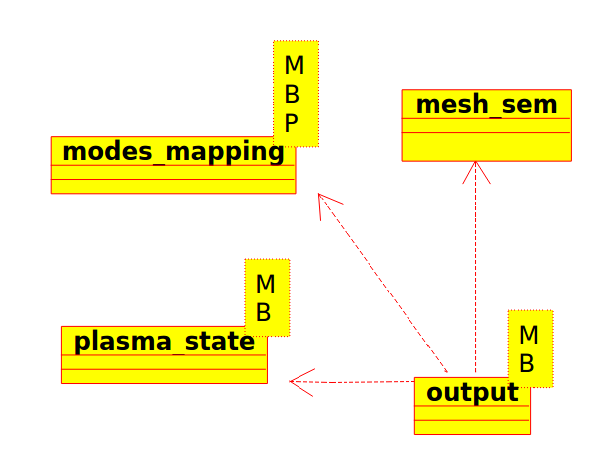
\includegraphics[scale=0.4]{images/output_diagram.png}}
\caption{Dumping: classes structure.}\label{fig:output_diagram}
\end{figure}

The class \verb|output| has three methods to perform the dump on file:
\begin{itemize}
  \item \verb|gmsh_dump(file_name)|: this method write, for each process, a file which contains the local portion of the mesh and the nodal values of the solution using the \verb|GMSH| format.
  \item \verb|dump(file_name,all_values)|: this method write, for each process, a file with contains, for each row, the $x$ coordinate, the $y$ coordinate and the value $\psi_{\delta}(x,y)$. If \verb|all_values| is set to \verb|false| only the nodal values are dumped, otherwise it sample for each elements the values of the solution on a structured mesh defined on the logical element. The sample points are equispaced and their number, for each element, is $(\max_m(p_m)+1\big)^2$. The points shared among different elements are write only once.
  \item \verb|dump_binary(file_name,all_values)|: this method is the same of \verb|dump| but, instead of using a unique file, it dumps the $x$ coordinate, the $y$ coordinate and the value $\psi_{\delta}(x,y)$ in three different files and the data are stored in binary format.
\end{itemize}

The solution values are extracted using the methods \verb|get_nodal_value(j)| and \verb|get_sol(j)| of the class \verb|plasma_state|.
\medskip

The class \verb|plasma_state| stores the values of the solutions. The nodal values are stored in a vector while a matrix stores in each row the coordinates and the values of the solution at that point. These two data structures are filled using the method \verb|update(n)| where \verb|n| is the number of points in which we want to split the edge. Therefore if it is equal to 0 we are taking only the nodal values of the solution while if it is equal to 1 we are taking the 4 nodal values, 4 values in the middle of each edge and 1 value in the center of the square. These values are evaluated using the method \verb|u_sol(x,y,e)| of the class \verb|modes_mapping|.
\medskip

In the following we report some plots of our simulations. The two-dimensional plots are the one obtained with \verb|GMSH| therefore they contains only the nodal values of the solution. Instead the surface plots are obtained using \verb|MATLAB| therefore they contain also the higher modes. Since the surfce plots function of \verb|MATLAB| deals only with structured grid, we project our solution over a structured grid using a linear interpolation and than we plot that solution.

\section{Examples}\label{sec:exemples}
The aim of these simulations is to test the code in different situations to benchmark it, therefore the emphasis of the analysis is not on the physical interpretation of the results obtained. All the tests were run on a small cluster using 8 processes. The basis degree is 2 for each variable and it is equal in all the elements. The dimension of the mesh is also very small, order of thousands of elements, therefore we refined the initial partition 5 times that is more than sufficient with so small mesh. The time of computation change a lot from simulation to simulation since it is strongly dominated by the iterative linear solver and in some case the stiffness matrix is very bad conditioned; it ranges from less than 1 second up to hundreds of seconds on the small cluster used.

\subsection{Benchmark linear test case: Poisson equation}\label{subsec:ex_poisson}
We choose to benchmark the linear part of our code with the well known Poisson equation in the domain $[-1,1]\times[-1,1]$. More precisely we want to solve the following linear problem
\begin{equation}
  \begin{cases}
   -\Delta u=(1-x^2)(1-y^2)& \mathrm{in}\:\Omega\\
   u=0& \mathrm{on}\:\partial\Omega
  \end{cases}
\end{equation}
which has solution the following analytical solution
\begin{equation}
 u(\mathbf{x})=-2x^2-2y^2+4.
\end{equation}

The discrete formulation of the problem is
\begin{equation}
  \begin{split}
    &\sum_m \bigg\{\sum_j \psi_j \sum_n w_n\:\hat{\nabla}\hat{\phi}_j(\mathbf{\hat{x}}_n)J_{\mathbf{F}_m}^{-1}(\mathbf{\hat{x}}_n)J_{\mathbf{F}_m}^{-T}(\mathbf{\hat{x}}_n)\hat{\nabla}\hat{\phi}_i(\mathbf{\hat{x}}_n)|\det(J_{\mathbf{F}_m}(\mathbf{\hat{x}}_n))|\bigg\}=\\
    &=0, \qquad\forall i\in\mathcal{I}
  \end{split}
\end{equation}
and is defined in the class \verb|poisson.h|.
\medskip

The mesh used is a structured one and it consists 4096 elements and 4230 nodes. The linear solver is the one used by default by \verb|PETSc|, the GMRES iterative method, while the preconditioner is the matrix itself with the flag \verb|DIFFERENT_NONZERO_PATTERN| which means that the preconditioning matrix does not have the same nonzero pattern structure during successive linear solves. We set two tolerances to test the convergence of the method: $10^{-15}$ for the decrease of the residual norm relative to the norm of the right hand side and for the absolute size of the residual norm while for the relative increase in the residual we set \verb|PETSC_DEFAULT|. Finally the maximum number of iterations is $10^4$. The plots of the numerical solution are reported in Fig.(\ref{fig:poisson}).

\begin{figure}
\centering
\subfigure{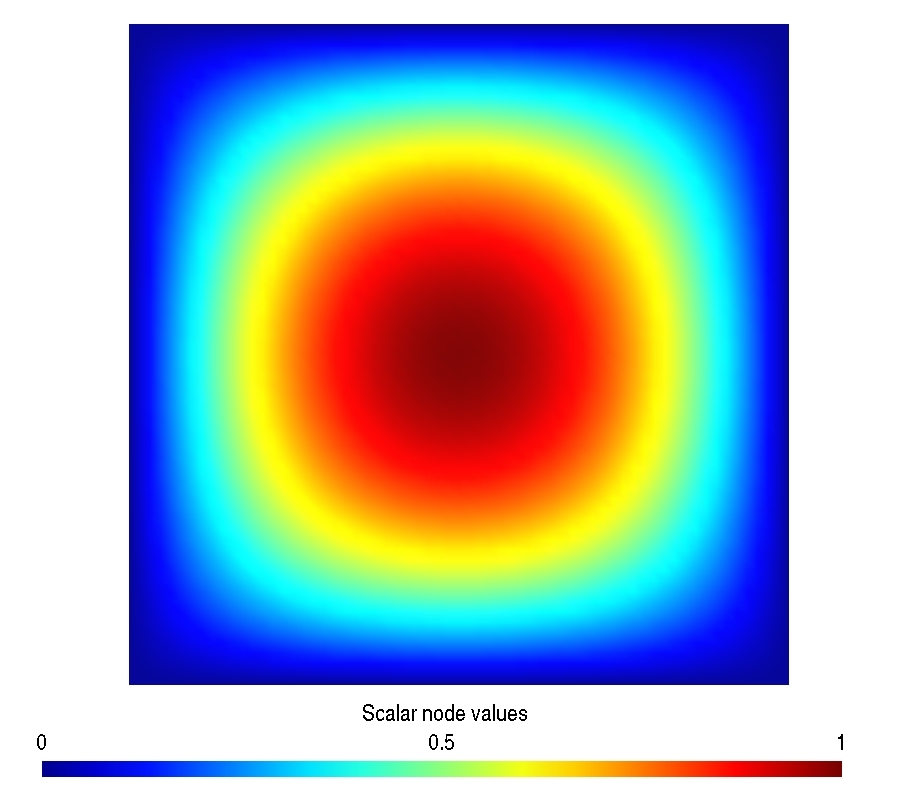
\includegraphics[scale=0.2]{images/poisson.jpg}}
\subfigure{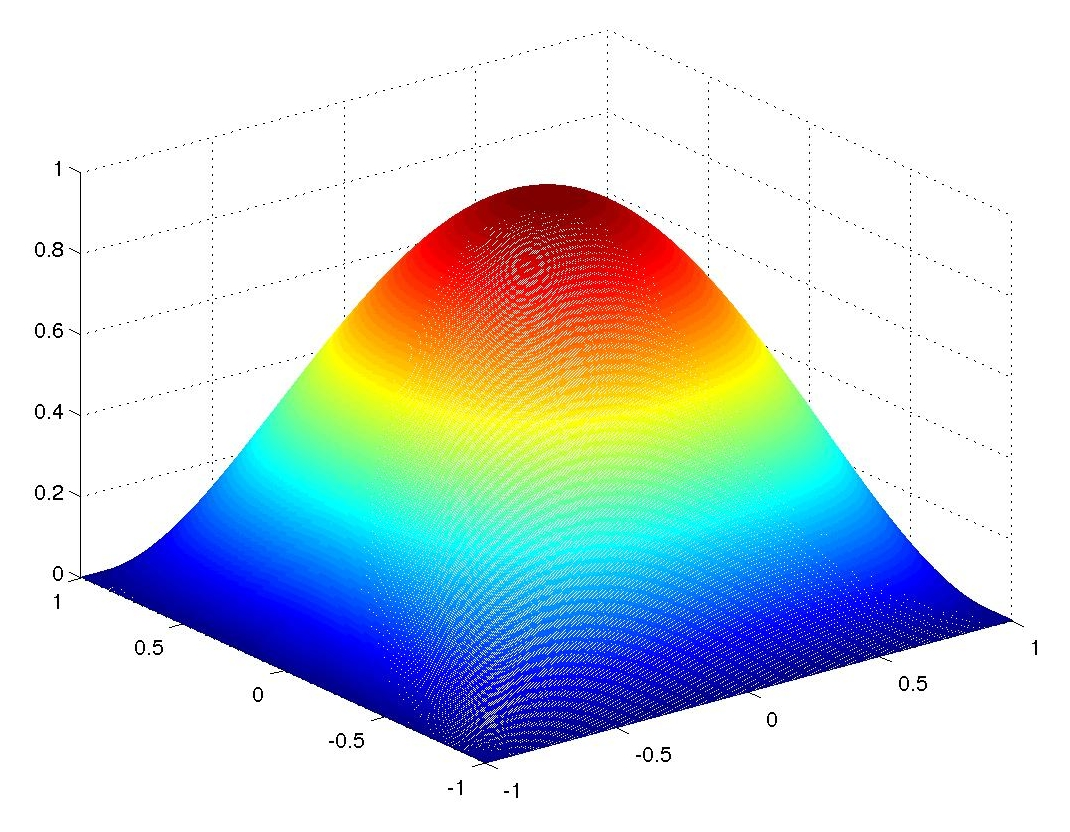
\includegraphics[scale=0.2]{images/poisson_surf.jpg}}
\caption{Discrete solution of the Poisson equation.}\label{fig:poisson}
\end{figure}

Since the analytical solution is a second order polynomial, in each variable,  we aspect to reach the precision of the machine since we are using a second order basis and Gaussian quadrature formula exact to the second order. This is indeed the case since
\begin{equation}
\|\mathbf{u}-\mathbf{u}_{\delta}\|_{\infty}=1.0170\cdot 10^{-13}
\end{equation}
where $\mathbf{u}$ is the vector of the exact solution evaluated in the points used to plot the surface while $\mathbf{u}_{\delta}$ are the discrete ones. This result tell us that the code works fine in the test case.

\subsection{Solution of the Grad-Shavranov operator}\label{subsec:ex_gs_operator}
We start to solve our problem, cmp. Eq.(\ref{eq:compact_equlibrium}), in the mirror domain shown in Fig.(\ref{fig:mirror_domain}) with the following parallel pressure profile
\begin{equation}
  p_{\|}(\psi,B)=0.
\end{equation}
Using this profile we obtain
\begin{equation}
  \begin{cases}
    \mathbf{F}(r,z,B,\psi,\nabla B, \nabla\psi)=0\\
     f(r,z,B,\psi)=0
  \end{cases}
\end{equation}
and the problem (\ref{eq:compact_equlibrium}) becomes
\begin{equation}
  \begin{cases}
    -\Delta^*\psi=0 & \mathrm{in}\:\Omega\\
    \psi(z,\gamma(z))=2\\
    \psi(0,r)=\psi(1,r)\\
    \nabla\psi(0,r)=\nabla\psi(1,r)
  \end{cases}
\end{equation}
which is linear. The discrete formulation of the problem is
\begin{equation}
  \begin{split}
    &\sum_m \bigg\{\sum_j \psi_j \sum_n w_n\:\mathbf{F}_m^r(\mathbf{\hat{x}}_n)\hat{\nabla}\hat{\phi}_j(\mathbf{\hat{x}}_n)J_{\mathbf{F}_m}^{-1}(\mathbf{\hat{x}}_n)J_{\mathbf{F}_m}^{-T}(\mathbf{\hat{x}}_n)\hat{\nabla}\hat{\phi}_i(\mathbf{\hat{x}}_n)|\det(J_{\mathbf{F}_m}(\mathbf{\hat{x}}_n))| +\\
    &+2\:\sum_j\psi_j\sum_n w_n[\frac{\partial\hat{x}}{\partial r},\frac{\partial\hat{y}}{\partial r}]_{\big|_{\mathbf{\hat{x}}_n}}\hat{\nabla} \hat{\phi}_j(\mathbf{\hat{x}}_n)\:\hat{\phi}_i(\mathbf{\hat{x}}_n)|\det(J_{\mathbf{F}_m}(\mathbf{\hat{x}}_n))|\bigg\}=0, \qquad\forall i\in\mathcal{I}
  \end{split}
\end{equation}
and is defined in the class \verb|lineargradshavranov.h|.
\medskip

The mesh used is an unstructured one and it consists of 2250 elements and 2159 nodes; we used the algorithm frontal of \verb|GMSH| starting from a boundary discretized with 92 nodes. The settings of the linear solver are the same of the ones used in the benchmark of the nonlinear problem, cmp.(\ref{subsec:ex_poisson}).The plots of the numerical solution are reported in Fig.(\ref{fig:gs_linear}).

\begin{figure}
\centering
\subfigure{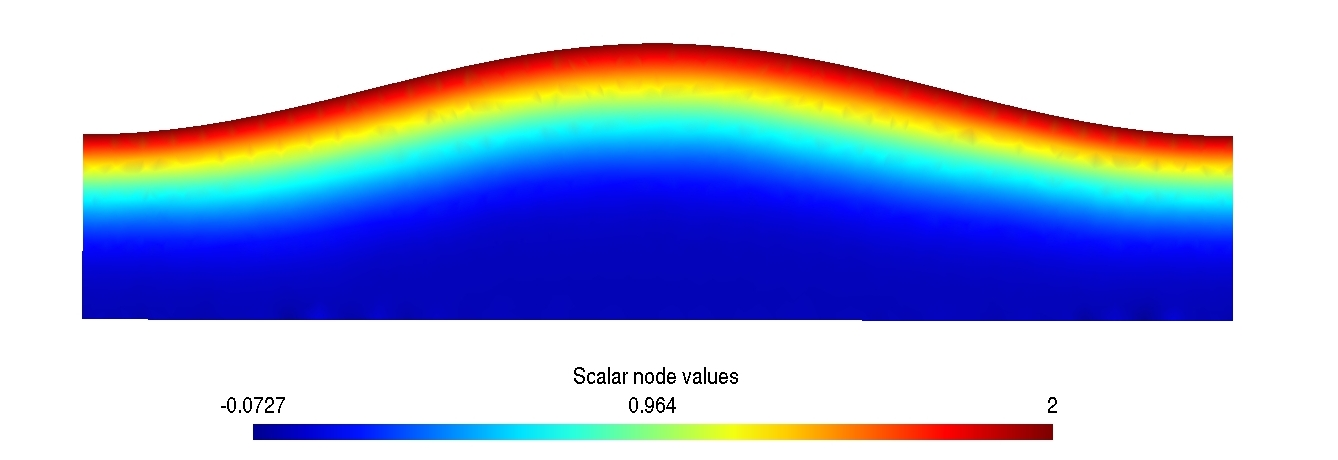
\includegraphics[scale=0.3]{images/gs_linear_nbc.jpg}}
\subfigure{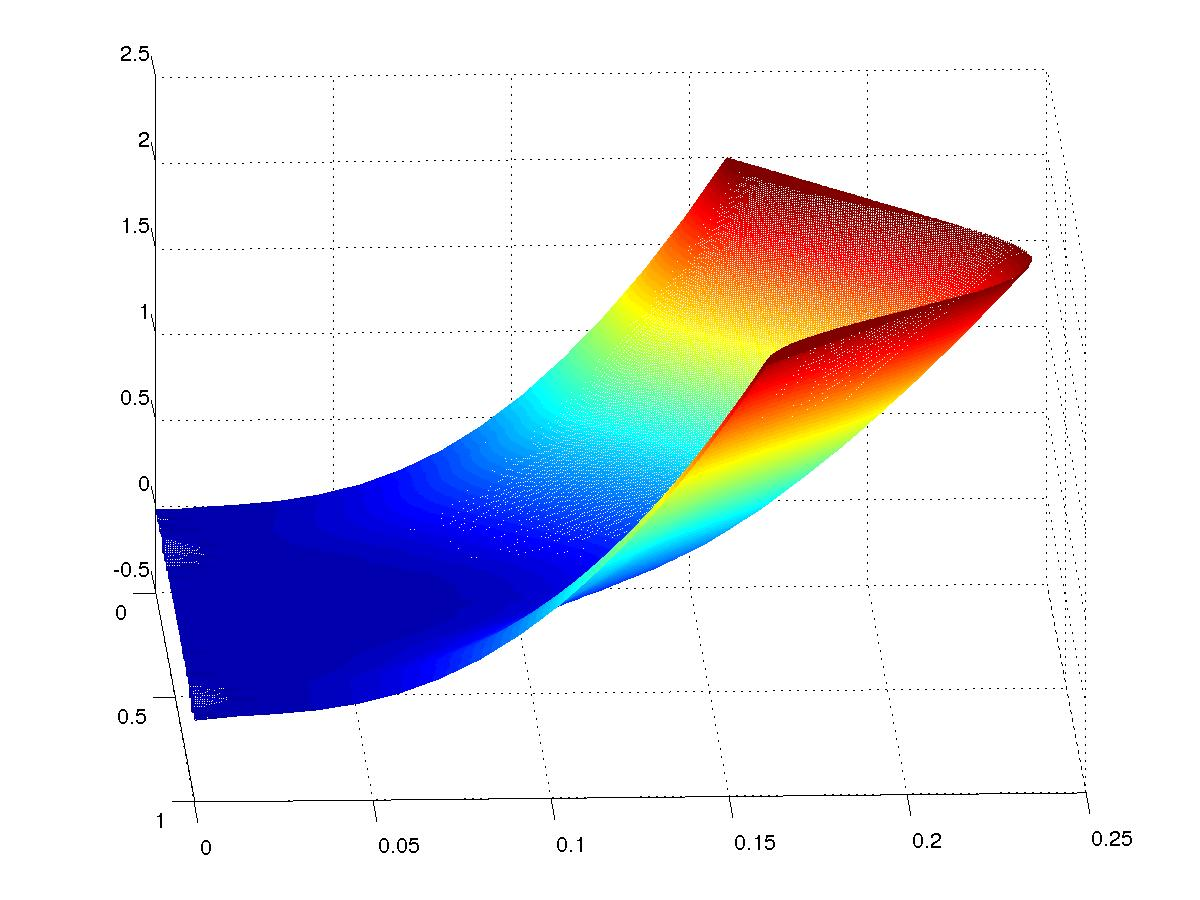
\includegraphics[scale=0.3]{images/gs_linear_nbc_surf.jpg}}
\caption{Discrete solution of the Grad-Shavranov operator.}\label{fig:gs_linear}
\end{figure}

The variable $\psi$ has not significant physical meaning itself indeed it is just a label for the magnetic field lines. Therefore the solution plotted in Fig.(\ref{fig:gs_linear}) represent the shape of the magnetic field lines in the special case of absence of parallel pressure.
\newpage

\subsection{Liner Grad-Shavranov problem}
We now solve our problem, cmp. Eq.(\ref{eq:compact_equlibrium}), in the inner tokamak domain with the following parallel pressure profile
\begin{equation}
  p_{\|}(\psi,B)=\frac{\partial}{\partial\psi}\bigg(p_0\big(1-\frac{\psi^2}{\psi_0^2}\big)\bigg).
\end{equation}
Using this profile we obtain
\begin{equation}
  \begin{cases}
    \mathbf{F}(r,z,B,\psi,\nabla B, \nabla\psi)=0\\
     f(r,z,B,\psi)=-2\frac{p_0}{\psi^2_0}\psi
  \end{cases}
\end{equation}
and the problem (\ref{eq:compact_equlibrium}) becomes
\begin{equation}
  \begin{cases}
    -\Delta^*\psi+2\frac{p_0}{\psi^2_0}r^2\psi=0 & \mathrm{in}\:\Omega\\
    \psi(z,\gamma(z))=2\\
    \psi(0,r)=\psi(1,r)\\
    \nabla\psi(0,r)=\nabla\psi(1,r)
  \end{cases}
\end{equation}
which is linear. The discrete formulation of the problem is
\begin{equation}
  \begin{split}
    &\sum_m \bigg\{\sum_j \psi_j \sum_n w_n\:\mathbf{F}_m^r(\mathbf{\hat{x}}_n)\hat{\nabla}\hat{\phi}_j(\mathbf{\hat{x}}_n)J_{\mathbf{F}_m}^{-1}(\mathbf{\hat{x}}_n)J_{\mathbf{F}_m}^{-T}(\mathbf{\hat{x}}_n)\hat{\nabla}\hat{\phi}_i(\mathbf{\hat{x}}_n)|\det(J_{\mathbf{F}_m}(\mathbf{\hat{x}}_n))| +\\
    &+2\:\sum_j\psi_j\sum_n w_n[\frac{\partial\hat{x}}{\partial r},\frac{\partial\hat{y}}{\partial r}]_{\big|_{\mathbf{\hat{x}}_n}}\hat{\nabla} \hat{\phi}_j(\mathbf{\hat{x}}_n)\:\hat{\phi}_i(\mathbf{\hat{x}}_n)|\det(J_{\mathbf{F}_m}(\mathbf{\hat{x}}_n))|+\\
    &+2\sum_n w_n\:\frac{p_0}{\psi^2_0}\mathbf{F}_m^r(\mathbf{\hat{x}}_n)^3 \hat{\phi}_j(\mathbf{\hat{x}}_n)\hat{\phi}_i(\mathbf{\hat{x}}_n)|\det(J_{\mathbf{F}_m}(\mathbf{\hat{x}}_n))|\bigg\}=0, \qquad\forall i\in\mathcal{I}
  \end{split}
\end{equation}
and is defined in the class \verb|lineargradshavranovmod.h|.
\medskip

The mesh used is an unstructured one and it consists 28752 elements and 28437 nodes; we used the algorithm Delaunay of \verb|GMSH| starting from a boundary discretized with 73 nodes and performing two refinements by splitting. The linear solver is the one used by default by \verb|PETSc|. No preconditioner has been used. We set two tolerances to test the convergence of the method: $10^{-15}$ for the decrease of the residual norm relative to the norm of the right hand side and for the absolute size of the residual norm while for the relative increase in the residual we set \verb|PETSC_DEFAULT|. Finally the maximum number of iterations is $10^4$. We choose $\frac{p_0}{\psi^2_0}=1$. The plots of the numerical solution are reported in Fig.(\ref{fig:gs_linear_mod}).

\begin{figure}
\centering
\subfigure{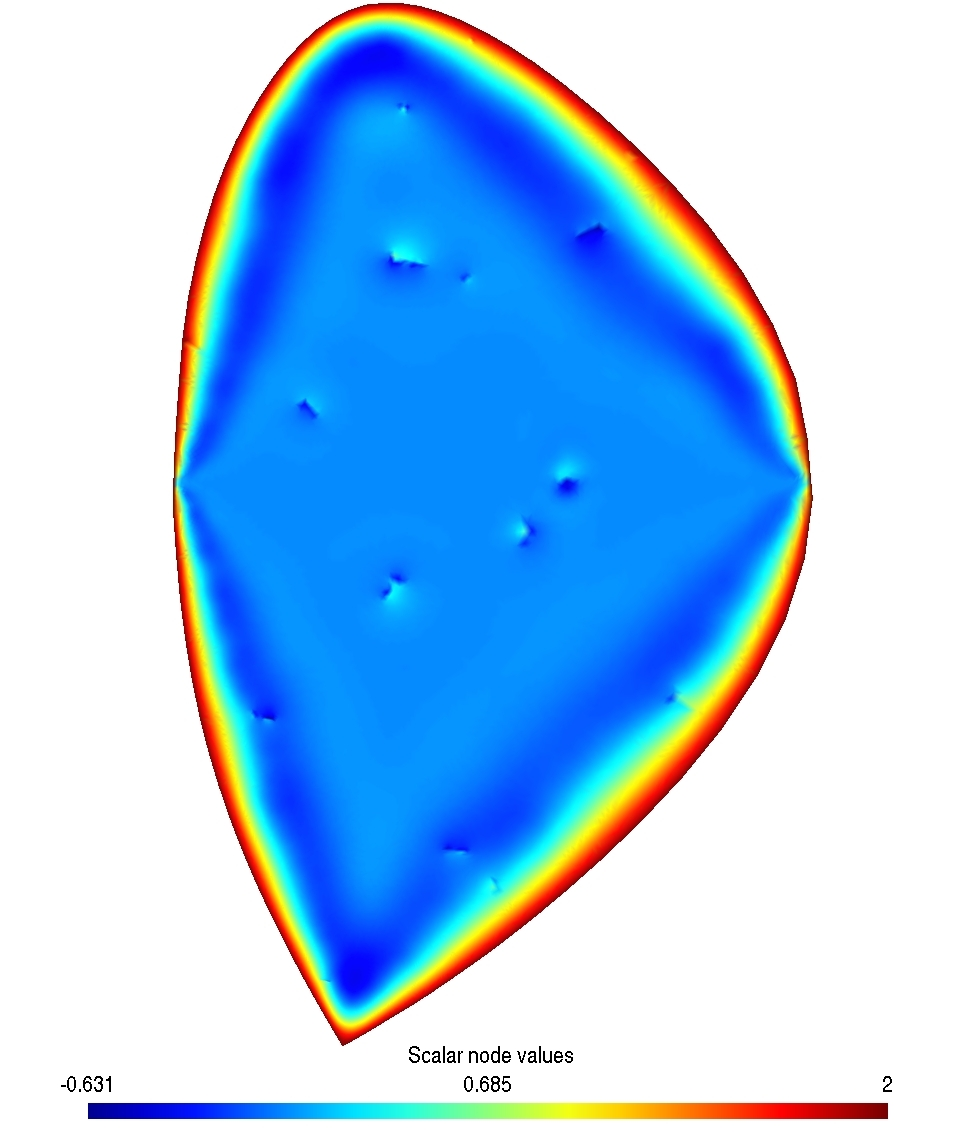
\includegraphics[scale=0.3]{images/gs_linear_mod_bis.jpg}}
\subfigure{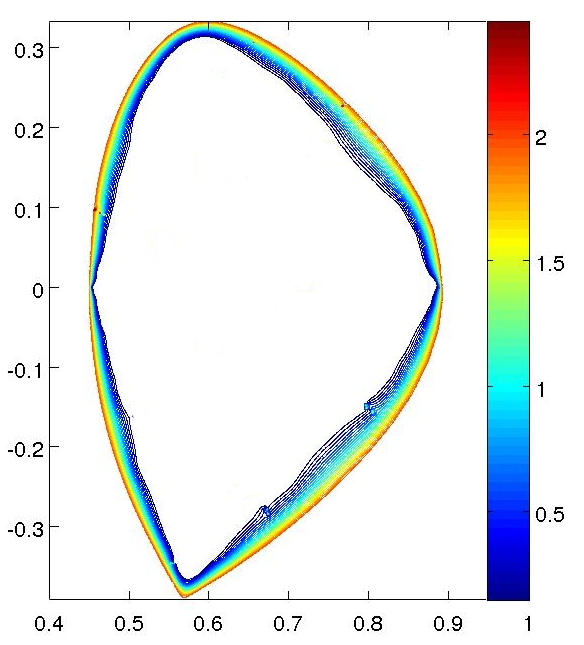
\includegraphics[scale=0.3]{images/gs_linear_mod_bis_countur.jpg}}
\caption{Discrete solution of the linear Grad-Shavranov problem and its countur plot.}\label{fig:gs_linear_mod}
\end{figure}

Unfortunately the problem is vary bad conditioned and the residual of the iterative solver decrease very slowly and it doesn't reach the tolerance requested also after all these iterations. We tried different preconditioner and different iterative solvers implemented in \verb|PETSc| but none of them works better. For this reason in Fig.(\ref{fig:gs_linear_mod}) we can see some noise due to the linear solver. We do not filtered it out to show where is localized the noise.

\subsection{Benchmark nonlinear test case: Bratu equation}
We choose to benchmark the nonlinear part of our code with the classical Bratu equation in the domain $[-1,1]\times[-1,1]$. More precisely we want to solve the following nonlinear problem
\begin{equation}
  \begin{cases}
   -\Delta u=\lambda e^{u}\qquad\mathrm{in}\:\Omega\\
   u=0\qquad\mathrm{on}\:\partial\Omega.
  \end{cases}
\end{equation}
Using the formalism introduced in Sec.(\ref{subsec:newton_method}) we have the following non linear functional $F$ defined as
\begin{equation}
  F(u)=\int_\Omega \big(\nabla u \cdot\nabla v-\lambda v\:e^{u}\big)\mathrm{d}\Omega
\end{equation}
and its Gateaux derivative is
\begin{equation}
  \mathcal{F}(u)\delta u=\int_\Omega \big(\nabla\delta u \cdot\nabla v-\lambda v\delta u\:e^{u}\big)\mathrm{d}\Omega.
\end{equation}

The discrete formulation of the problem is
\begin{equation}
  \begin{split}
    &F\big(u^{(k)}(\mathbf{x})\big)=\\
    &=\sum_m \bigg\{\sum_n w_n\:\hat{\nabla}\hat{u}^{(k)}(\mathbf{\hat{x}}_n)J_{\mathbf{F}_m}^{-1}(\mathbf{\hat{x}}_n)J_{\mathbf{F}_m}^{-T}(\mathbf{\hat{x}}_n)\hat{\nabla}\hat{\phi}_i(\mathbf{\hat{x}}_n)|\det(J_{\mathbf{F}_m}(\mathbf{\hat{x}}_n))|+\\
    &+\sum_n w_n\:\lambda\:\hat{\phi}_i(\mathbf{\hat{x}}_n)e^{\hat{u}^{(k)}(\mathbf{\hat{x}}_n)}|\det(J_{\mathbf{F}_m}(\mathbf{\hat{x}}_n))|\bigg\},\qquad\forall i\in\mathcal{I};
  \end{split}
\end{equation}
\begin{equation}
  \begin{split}
    &\mathcal{F}(u^{(k)})\bigg(\sum_j\delta u_j\phi_j(\mathbf{x})\bigg)=\\
    &=\sum_m \bigg\{\sum_j \delta u_j \sum_n w_n\:\hat{\nabla}\hat{\phi}_j(\mathbf{\hat{x}}_n)J_{\mathbf{F}_m}^{-1}(\mathbf{\hat{x}}_n)J_{\mathbf{F}_m}^{-T}(\mathbf{\hat{x}}_n)\hat{\nabla}\hat{\phi}_i(\mathbf{\hat{x}}_n)|\det(J_{\mathbf{F}_m}(\mathbf{\hat{x}}_n))|+\\
    &+\sum_j \delta u_j \sum_n w_n\:\lambda\:\hat{\phi}_i(\mathbf{\hat{x}}_n)e^{\hat{u}^{(k)}(\mathbf{\hat{x}}_n)}\hat{\phi}_j(\mathbf{\hat{x}}_n)|\det(J_{\mathbf{F}_m}(\mathbf{\hat{x}}_n))|\bigg\},\qquad\forall i\in\mathcal{I},
  \end{split}
\end{equation}
and is defined in the class \verb|bratu.h|.
\medskip

The mesh used and the settings of the linear solver are the same of the ones used in the benchmark of the nonlinear problem, cmp.(\ref{subsec:ex_poisson}). We set the tolerance of the nonlinear solver equal to $10^{-7}$ and the maximum number of iteration is 50. We choose $\lambda=1$. The plots of the numerical solution are reported in Fig.(\ref{fig:poisson}).

\begin{figure}
\centering
\subfigure{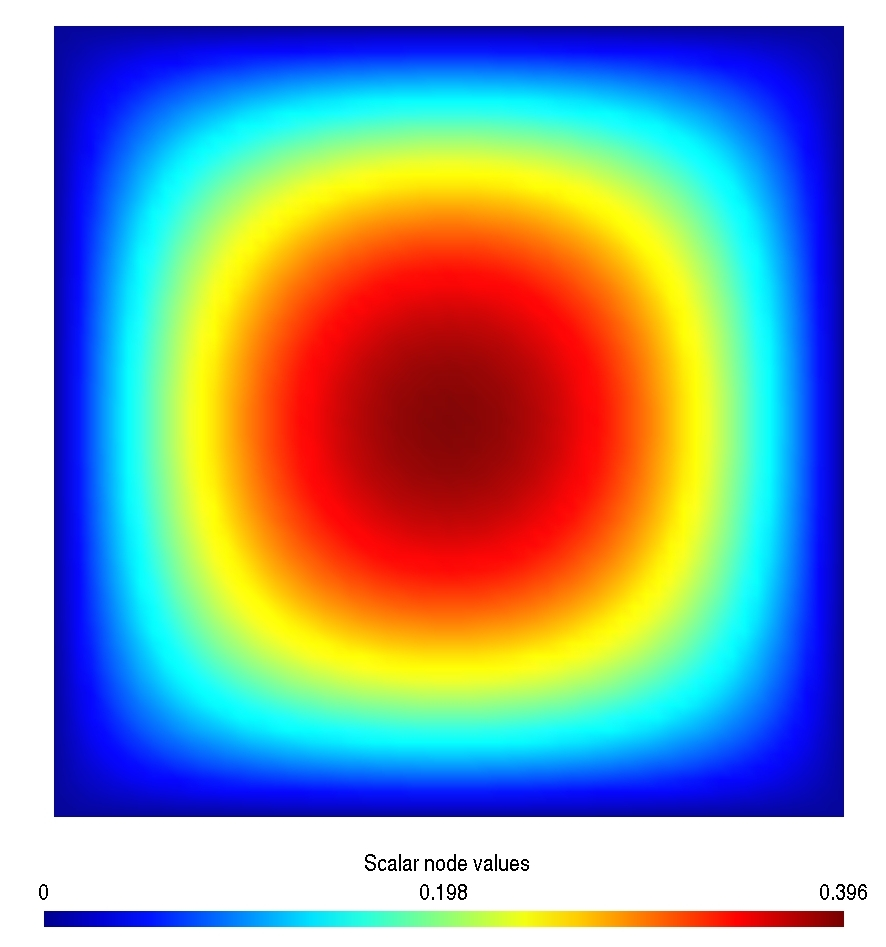
\includegraphics[scale=0.2]{images/bratu.jpg}}
\subfigure{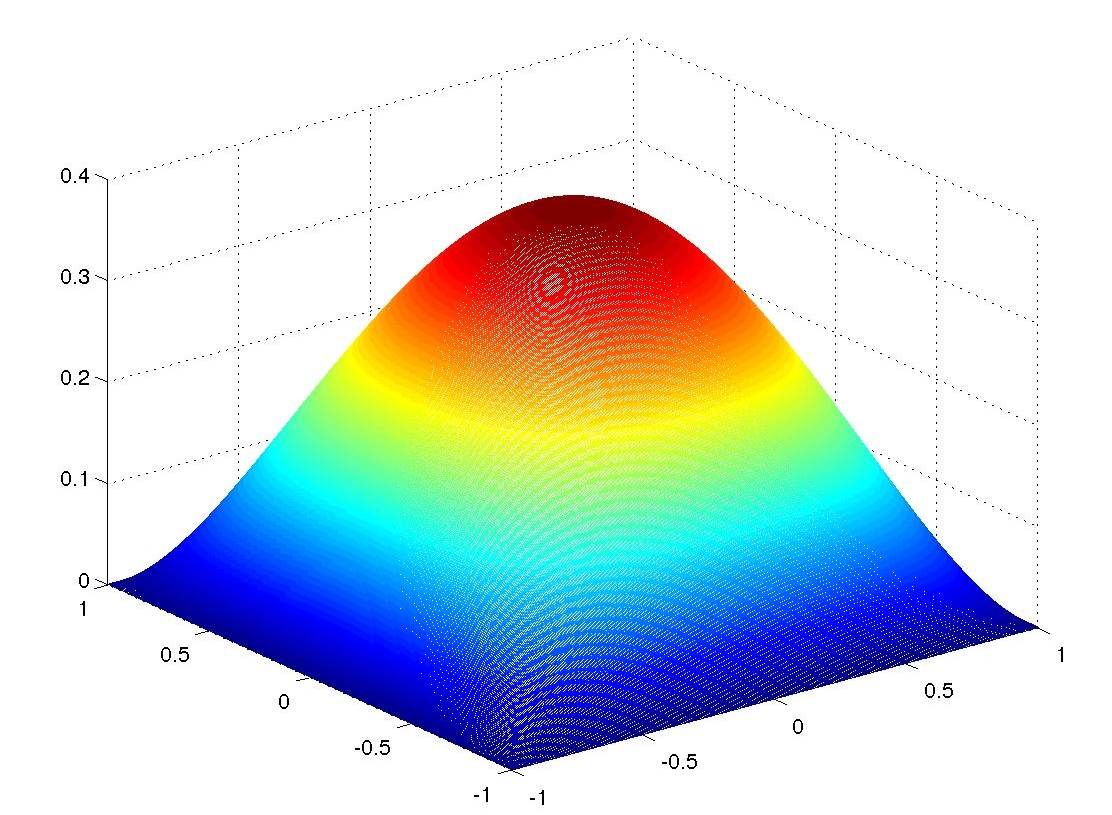
\includegraphics[scale=0.2]{images/bratu_surf.jpg}}
\caption{Discrete solution of the Bratu equation.}\label{fig:bratu}
\end{figure}

In Fig.(\ref{fig:bratu_norm}) we plot the dependence of the residual from the initial guess. More precisely, the x-axis shows the iteration step of the nonlinear solver while the y-axis shows, in logarithmic scale, the value of the residual $\|F(u^{(n)})\|_{L^2(\Omega)}$. We report three different initial guess: $u^{(0)}(\mathbf{x})=0$ in red, $u^{(0)}(\mathbf{x})=1$ in green and $u^{(0)}(\mathbf{x})=0$ in blue. The initial guess is set only on the degrees of freedom of the problem while on the Dirichlet boundary are set the right values of the solution.

\begin{figure}
\centering
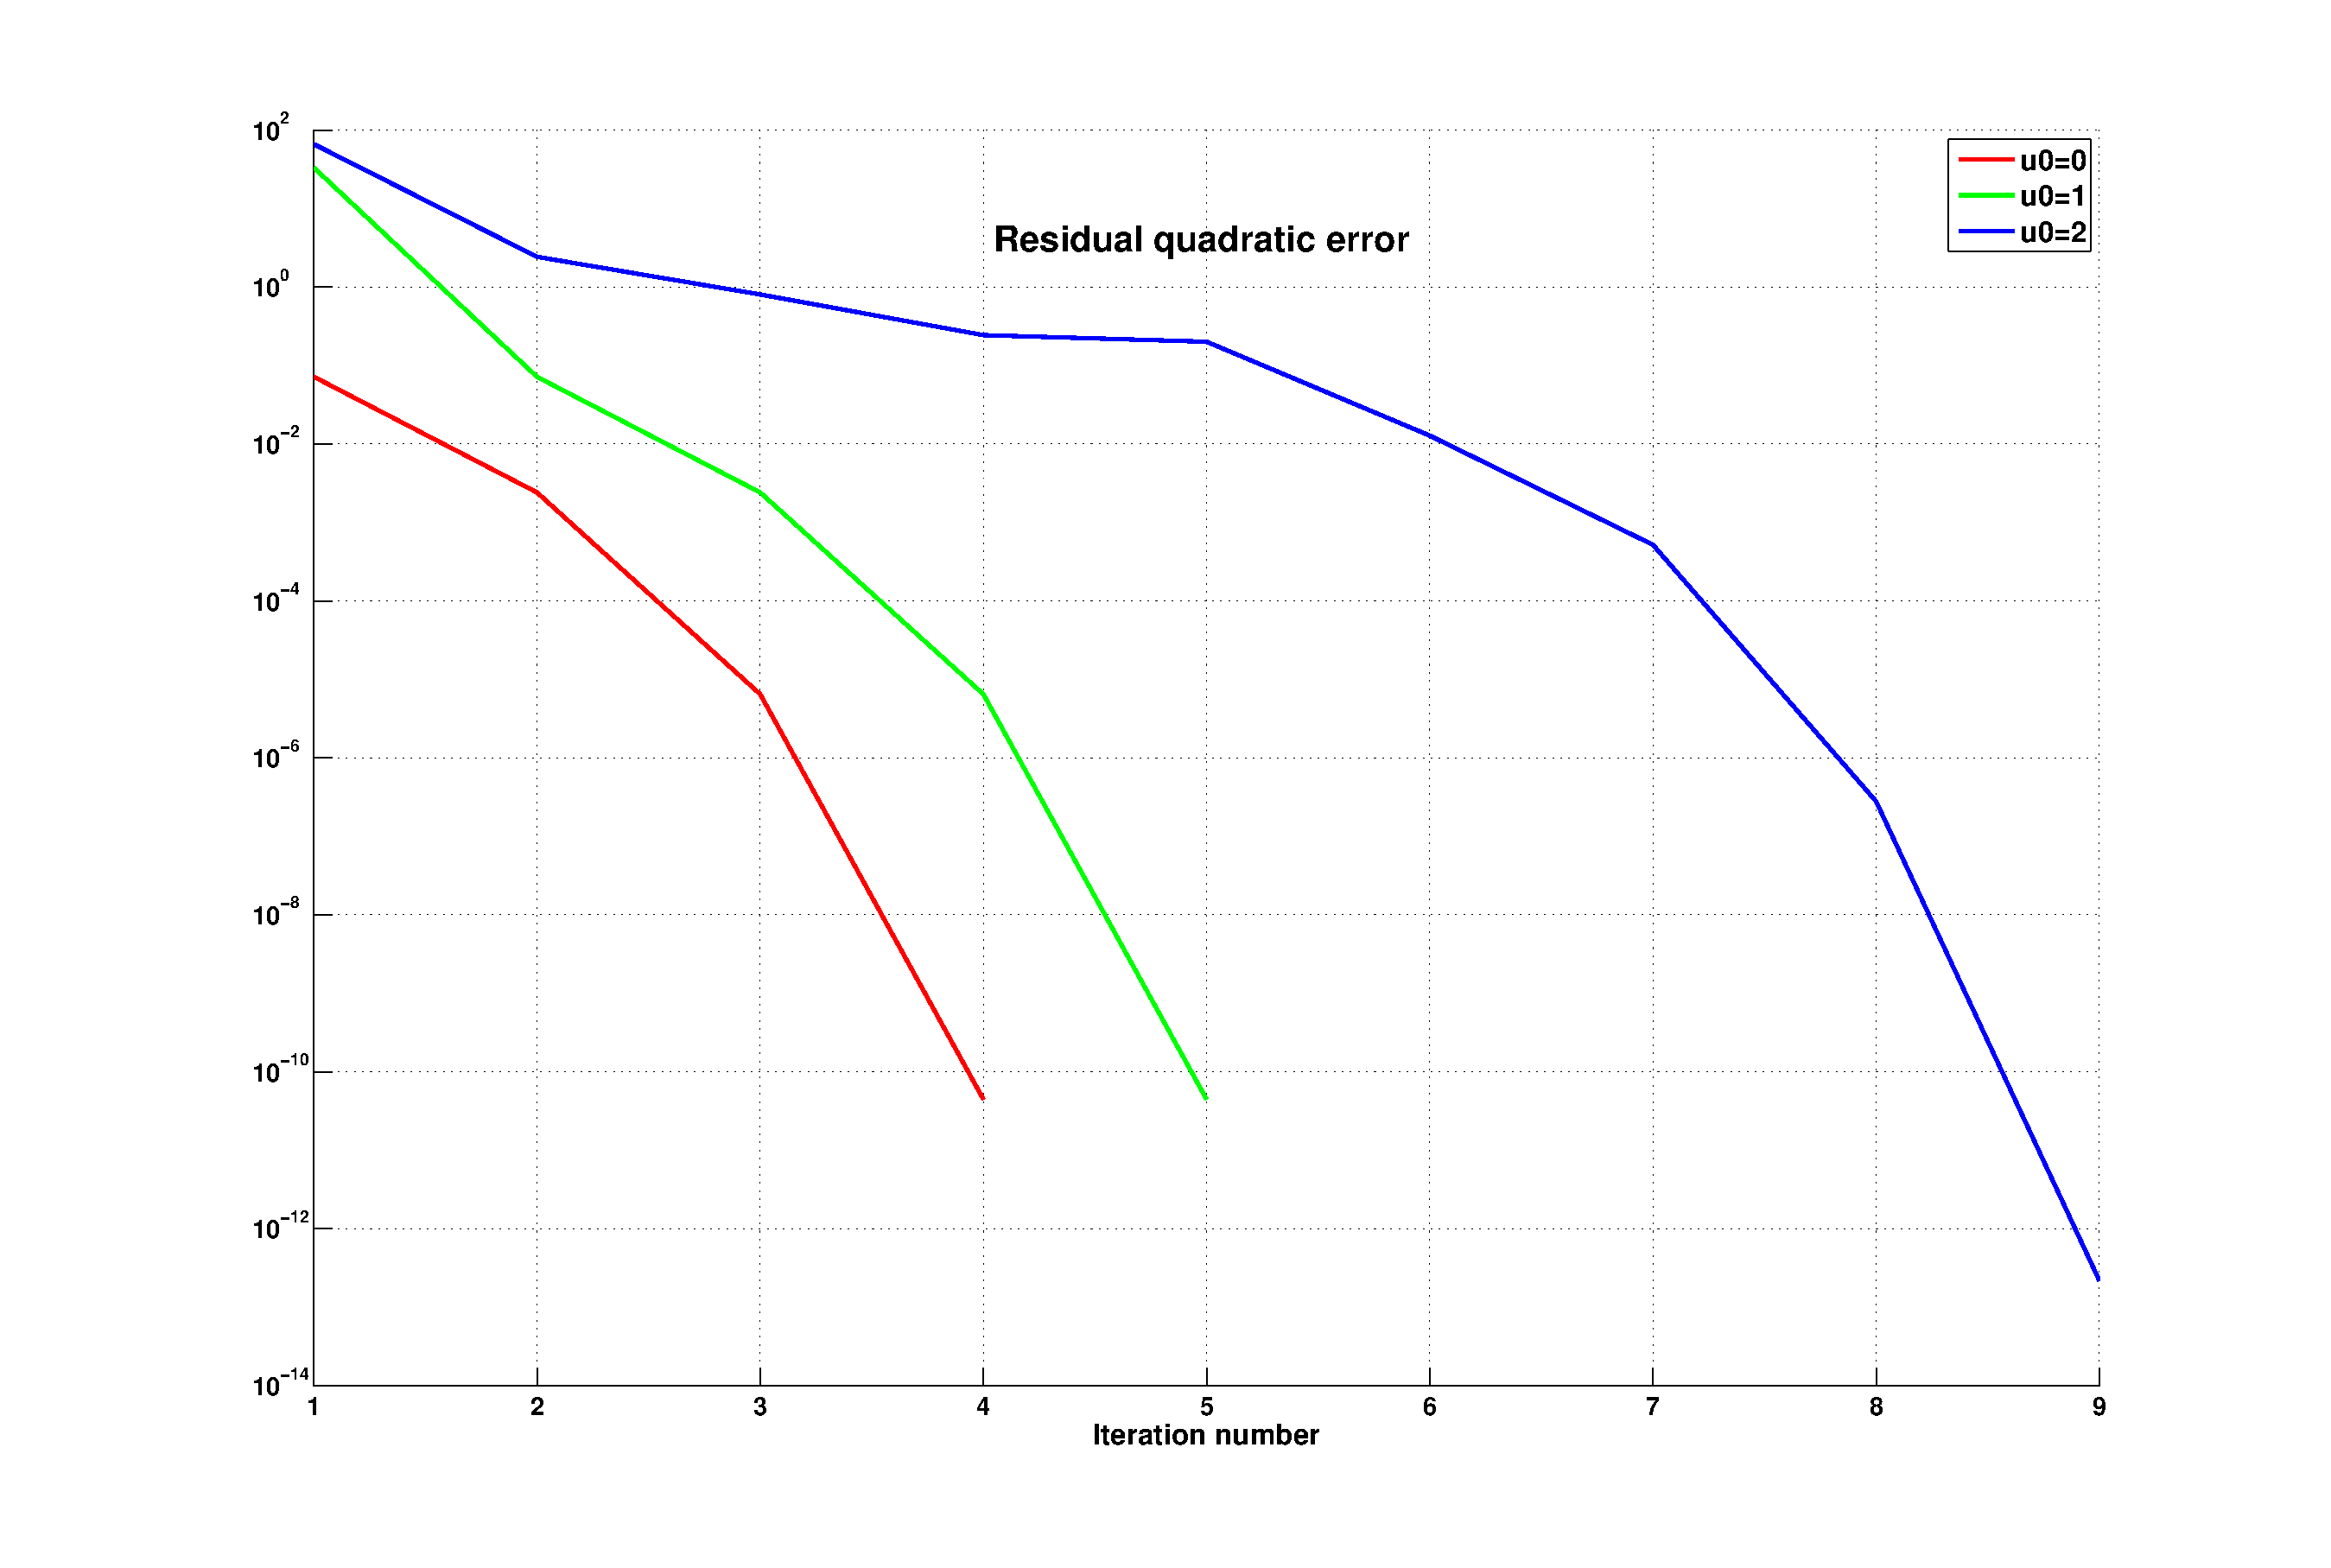
\includegraphics[scale=0.3]{images/bratu_norm.eps}
\caption{Dependence of the residual $\|F(u^{(n)})\|_{L^2(\Omega)}$ from the initial guess.}\label{fig:bratu_norm}
\end{figure}

We can notice that, in both 3 cases, the desired tolerance is reached way before the maximum number of iterations but also that varying a little the initial guess, the number of iteration can change considerably. The nonlinear solver part, which is built over the linear solver code, reaching the tolerance of the residual in a small number of iteration, works fine in the test case.

\subsection{Nonlinear Grad-Shavranov}
We now solve our problem, cmp. Eq.(\ref{eq:compact_equlibrium}), in the mirror domain shown in Fig.(\ref{fig:mirror_domain}) with the following parallel pressure profile
\begin{equation}
  f(r,z,B,\psi)=p_0\big(1-\frac{\psi^2}{\psi^2_0}\big).
\end{equation}
Using this profile, the problem (\ref{eq:compact_equlibrium}) becomes
\begin{equation}
  \begin{cases}
    -\Delta^*\psi-p_0\:r^2\:\big(1-\frac{\psi^2}{\psi^2_0}\big)=0 & \mathrm{in}\:\Omega\\
    \psi(z,\gamma(z))=2\\
    \psi(0,r)=\psi(1,r)\\
    \nabla\psi(0,r)=\nabla\psi(1,r)
  \end{cases}
\end{equation}
which is nonlinear. Using the formalism introduce in Sec.(\ref{subsec:newton_method}) we have the following non linear functional $F$ defined as
\begin{equation}
  F(\psi)=\int_\Omega \bigg(r\:\nabla \psi \cdot\nabla v+2\:v\:\partial_r\psi-r^3\:p_0\big(1-\frac{\psi^2}{\psi^2_0}\big)\bigg)\mathrm{d}\Omega
\end{equation}
and its Gateaux derivative is
\begin{equation}
  \mathcal{F}(\psi)\delta \psi=\int_\Omega \bigg(r\:\nabla \delta\psi \cdot\nabla v+2\:v\:\partial_r\delta\psi+2\frac{p_0}{\psi^2_0}\:r^3v\:\psi\delta\psi\bigg)\mathrm{d}\Omega.
\end{equation}

The discrete formulation of the problem is
\begin{equation}
  \begin{split}
    &F\big(\psi^{(k)}(\mathbf{x})\big)=\\
    &\sum_m \bigg\{\sum_n w_n\:\mathbf{F}_m^r(\mathbf{\hat{x}}_n)\hat{\nabla}\hat{\psi}^{(k)}(\mathbf{\hat{x}}_n)J_{\mathbf{F}_m}^{-1}(\mathbf{\hat{x}}_n)J_{\mathbf{F}_m}^{-T}(\mathbf{\hat{x}}_n)\hat{\nabla}\hat{\phi}_i(\mathbf{\hat{x}}_n)|\det(J_{\mathbf{F}_m}(\mathbf{\hat{x}}_n))| +\\
    &+2\:\sum_n w_n[\frac{\partial\hat{x}}{\partial r},\frac{\partial\hat{y}}{\partial r}]_{\big|_{\mathbf{\hat{x}}_n}}\hat{\nabla} \hat{\psi}^{(k)}(\mathbf{\hat{x}}_n)\:\hat{\phi}_i(\mathbf{\hat{x}}_n)|\det(J_{\mathbf{F}_m}(\mathbf{\hat{x}}_n))|+\\
    &-\sum_n w_n\:p_0\:\mathbf{F}_m^r(\mathbf{\hat{x}}_n)^3 \bigg(1-\bigg(\frac{\hat{\psi}^{(k)}}{\psi_0}\bigg)^2\bigg)\hat{\phi}_i(\mathbf{\hat{x}}_n)|\det(J_{\mathbf{F}_m}(\mathbf{\hat{x}}_n))|\bigg\}=0, \qquad\forall i\in\mathcal{I};
  \end{split}
\end{equation}
\begin{equation}
  \begin{split}
    &\mathcal{F}(\psi^{(k)})\bigg(\sum_j\delta \psi_j\phi_j(\mathbf{x})\bigg)=\\
    &\sum_m \bigg\{\sum_j \delta\psi_j \sum_n w_n\:\mathbf{F}_m^r(\mathbf{\hat{x}}_n)\hat{\nabla}\hat{\phi}_j(\mathbf{\hat{x}}_n)J_{\mathbf{F}_m}^{-1}(\mathbf{\hat{x}}_n)J_{\mathbf{F}_m}^{-T}(\mathbf{\hat{x}}_n)\hat{\nabla}\hat{\phi}_i(\mathbf{\hat{x}}_n)|\det(J_{\mathbf{F}_m}(\mathbf{\hat{x}}_n))| +\\
    &+2\:\sum_j\delta\psi_j\sum_n w_n[\frac{\partial\hat{x}}{\partial r},\frac{\partial\hat{y}}{\partial r}]_{\big|_{\mathbf{\hat{x}}_n}}\hat{\nabla} \hat{\phi}_j(\mathbf{\hat{x}}_n)\:\hat{\phi}_i(\mathbf{\hat{x}}_n)|\det(J_{\mathbf{F}_m}(\mathbf{\hat{x}}_n))|+\\
    &+2\sum_j\delta\psi_j\sum_n w_n\:\frac{p_0}{\psi_0^2}\mathbf{F}_m^r(\mathbf{\hat{x}}_n)^3\hat{\phi}_i(\mathbf{\hat{x}}_n)\hat{\psi}^{(k)}(\mathbf{\hat{x}}_n)\hat{\phi}_j(\mathbf{\hat{x}}_n)|\det(J_{\mathbf{F}_m}(\mathbf{\hat{x}}_n))|\bigg\}=0, \qquad\forall i\in\mathcal{I},
  \end{split}
\end{equation}
and is defined in the class \verb|gradshavranov.h|.
\medskip

The mesh used and the settings of the linear solver are the same of the ones used in Sec.(\ref{subsec:ex_gs_operator}). We set the tolerance of the nonlinear solver equal to $10^{-7}$ and the maximum number of iteration is 50. We choose $\psi^2_0=1$. The plots of the numerical solution are reported in Fig.(\ref{fig:gs}) where the first plot has $p_0=1$ while the second $p_0=1000$.

\begin{figure}
\centering
\subfigure{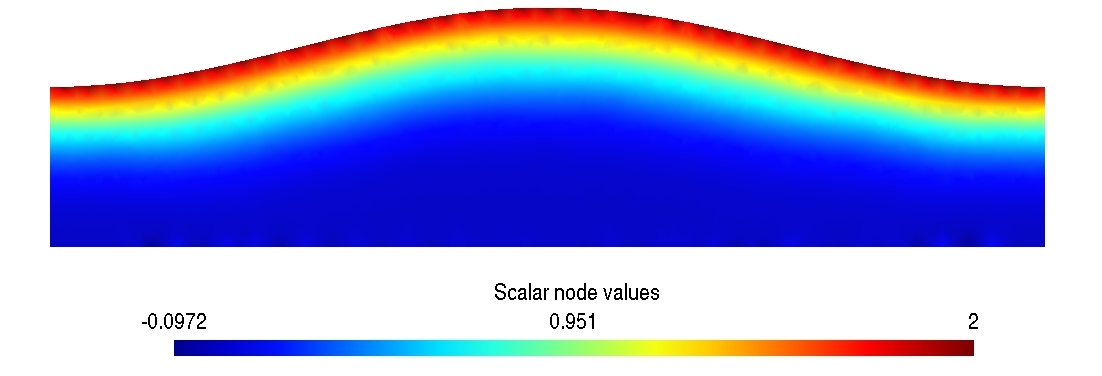
\includegraphics[scale=0.32]{images/gs.jpg}}
\subfigure{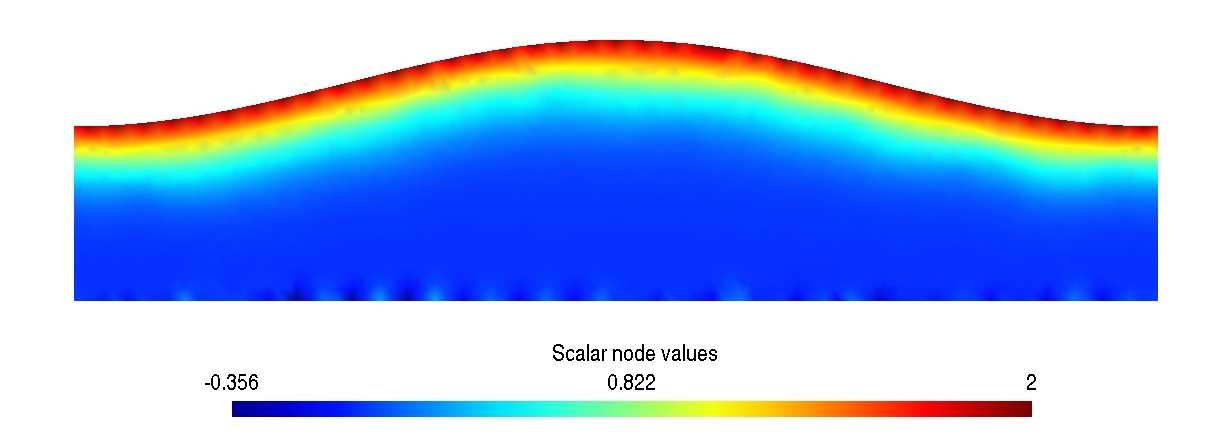
\includegraphics[scale=0.29]{images/gs_1000.jpg}}
\caption{Discrete solution of the nonlinear Grad-Shavranov problem with $p_0=1$ and $p_0=1000$.}\label{fig:gs}
\end{figure}

We can notice that when $p_0=1$ the solution is very close to the one shows in Sec.(\ref{subsec:ex_gs_operator}). That is not surprising indeed the function $ f(r,z,B,\psi)$ is multiplied by $r^3\propto10^{-3}$ therefore the nonlinearity influences the solution by a factor proportional to $\frac{1}{1000}$; instead, in the second case, the linear and the nonlinear term have the same order of magnitude and the solution is strongly influenced by the nonlinear term.


\appendix

\chapter{Some proofs}\label{ch:appx}
In this appendix we report all the passages missing in Sec.(\ref{sec:grad_shavranov}) to arrive at the Grad-Shavranov equation.

\section{Divergence of the pressure tensor}
Derivation of Eq.(\ref{eq:div_press}).
\begin{equation*}
  \begin{split}
    \nabla\cdot\mathbb{P}&=\nabla\cdot[p_\perp \mathbb{I} + ( p_\parallel - p_\perp ) \mathbf{b}\mathbf{b}]=
    \nabla\cdot(p_\perp \mathbb{I}) + \nabla\cdot[( p_\parallel - p_\perp ) \mathbf{b}\mathbf{b}]=\\
    &=\nabla p_\perp+(p_\parallel-p_\perp)\nabla\cdot(\mathbf{b}\mathbf{b})+\mathbf{b}\mathbf{b}\cdot\nabla(p_\parallel-p_\perp)=\\
    &=\nabla p_\perp+(p_\parallel-p_\perp)\nabla\cdot(\mathbf{b}\mathbf{b})+\mathbf{b}\big(\mathbf{b}\cdot\nabla(p_\parallel-p_\perp)\big)=\\
    &=\nabla p_\perp+(p_\parallel-p_\perp)[(\nabla\cdot\mathbf{b})\mathbf{b}+(\mathbf{b}\cdot\nabla)\mathbf{b}]+\big(\mathbf{b}\cdot\nabla(p_\parallel-p_\perp)\big)\mathbf{b}=\\
    &=\nabla p_\perp+(p_\parallel-p_\perp)\Big[\big(\nabla\cdot(B^{-1}\mathbf{B})\big)\mathbf{b}+\mathbf{k}\Big]+\big(\mathbf{b}\cdot\nabla(p_\parallel-p_\perp)\big)\mathbf{b}=\\
    &=\nabla p_\perp+(p_\parallel-p_\perp)\Big\{\big[\nabla B^{-1}\cdot\mathbf{B}+B^{-1}(\nabla\cdot\mathbf{B})\big]\mathbf{b}+\mathbf{k}\Big\}+\big(\mathbf{b}\cdot\nabla(p_\parallel-p_\perp)\big)\mathbf{b}=\\
    &\overset{\mbox{(\ref{eq:MHD_maxwell})}}{=}\nabla p_\perp+(p_\parallel-p_\perp)\Big\{\big[\nabla B^{-1}\cdot\mathbf{B}\big]\mathbf{b}+\mathbf{k}\Big\}+\big(\mathbf{b}\cdot\nabla(p_\parallel-p_\perp)\big)\mathbf{b}=\\
    &=\nabla p_\perp+(p_\parallel-p_\perp)\Big[\big( -B^{-2}\nabla B\cdot\mathbf{B}\big)\mathbf{b}+\mathbf{k}\Big]+\big(\mathbf{b}\cdot\nabla(p_\parallel-p_\perp)\big)\mathbf{b}=\\
    &=\nabla p_\perp+(p_\parallel-p_\perp)\Big[\big( -B^{-1}\nabla B\cdot\mathbf{b}\big)\mathbf{b}+\mathbf{k}\Big]+\big(\mathbf{b}\cdot\nabla(p_\parallel-p_\perp)\big)\mathbf{b}=\\
    &=\nabla p_\perp+(p_\parallel-p_\perp)\Big[ -B^{-1}\big(\nabla B\cdot\mathbf{b}\big)\mathbf{b}+\mathbf{k}\Big]+\big(\mathbf{b}\cdot\nabla(p_\parallel-p_\perp)\big)\mathbf{b}=\\
    &=\nabla p_\perp+(p_\parallel-p_\perp)\mathbf{k}+\Big[\mathbf{b}\cdot\nabla(p_\parallel-p_\perp)-B^{-1}(p_\parallel-p_\perp)\nabla B\cdot\mathbf{b}\Big]\mathbf{b}.
 \end{split}
\end{equation*}

\section{Pressure balance equation}
Derivation of Eq.(\ref{eq:pressure_balance}).
\medskip

It holds that
\begin{equation*}
  \mathbf{b} \cdot(\nabla\cdot\mathbb{P})=B^{-1}\mathbf{B}\cdot(\nabla\cdot\mathbb{P})\overset{\mbox{(\ref{eq:MHD_momentum})}}{=} B^{-1}\mathbf{B}\cdot(\nabla\times\mathbf{B})\times\mathbf{B}=B^{-1}(\nabla\times\mathbf{B})\cdot\mathbf{B}\times\mathbf{B}=0
\end{equation*}
and
\begin{equation*}
  \begin{split}
    \mathbf{b} \cdot(\nabla\cdot\mathbb{P}) &\overset{\mbox{(\ref{eq:div_press})}}{=}
    \mathbf{b}\cdot\bigg\{\nabla p_\perp+(p_\parallel-p_\perp)\mathbf{k}+\Big[\mathbf{b}\cdot\nabla(p_\parallel-p_\perp)-B^{-1}(p_\parallel-p_\perp)\nabla B\cdot\mathbf{b}\Big]\mathbf{b}\bigg\}=\\
    &=\mathbf{b}\cdot\nabla p_\perp+(p_\parallel-p_\perp)\mathbf{k}\cdot\mathbf{b}+\Big[\mathbf{b}\cdot\nabla(p_\parallel-p_\perp)-B^{-1}(p_\parallel-p_\perp)\nabla B\cdot\mathbf{b}\Big]\mathbf{b}\cdot\mathbf{b}=\\
    &=\mathbf{b}\cdot\nabla p_\perp+(p_\parallel-p_\perp)\mathbf{k}\cdot\mathbf{b}+\Big[\mathbf{b}\cdot\nabla(p_\parallel-p_\perp)-B^{-1}(p_\parallel-p_\perp)\nabla B\cdot\mathbf{b}\Big]B^{-2}\mathbf{B}\cdot\mathbf{B}=\\
    &=\mathbf{b}\cdot\nabla p_\perp+(p_\parallel-p_\perp)\mathbf{k}\cdot\mathbf{b}+\mathbf{b}\cdot\nabla(p_\parallel-p_\perp)-B^{-1}(p_\parallel-p_\perp)\nabla B\cdot\mathbf{b}=\\
    &=\mathbf{b}\cdot[\nabla p_\perp+\nabla(p_\parallel-p_\perp)]+(p_\parallel-p_\perp)\mathbf{k}\cdot\mathbf{b}-B^{-1}(p_\parallel-p_\perp)\nabla B\cdot\mathbf{b}=\\
    &=\mathbf{b}\cdot\nabla p_\parallel+(p_\parallel-p_\perp)\mathbf{k}\cdot\mathbf{b}-B^{-1}(p_\parallel-p_\perp)\nabla B\cdot\mathbf{b}=\\
    &\overset{\mbox{(\ref{eq:kb0})}}{=}\mathbf{b}\cdot\nabla p_\parallel-B^{-1}(p_\parallel-p_\perp)\nabla B\cdot\mathbf{b}=\\
    &=\mathbf{b}\cdot\nabla p_\parallel-B^{-1}(p_\parallel-p_\perp)\mathbf{b}\cdot\nabla B=\\
    &=(\mathbf{b}\cdot\nabla) p_\parallel-B^{-1}(p_\parallel-p_\perp)(\mathbf{b}\cdot\nabla) B=\\
    &=\frac{\partial p_\parallel}{\partial l} -B^{-1}(p_\parallel-p_\perp)\frac{\partial B}{\partial l}
  \end{split}
\end{equation*}
where $l$ is the arc length of $\mathbf{B}$ that increase in which $\mathbf{B}$ points, so $l$ measures the distance along the magnetic field-line, and
\begin{equation}\label{eq:kb0}
  \begin{split}
    \mathbf{k}\cdot\mathbf{b}&=(\mathbf{b}\cdot\nabla)\mathbf{b}\cdot\mathbf{b}=\sum_i(\sum_j b_j \frac{\partial b_i}{\partial x_j})b_i=\sum_i\sum_j b_j \frac{\partial b_i}{\partial x_j}b_i=\\
    &=\sum_i\sum_j b_j \frac{\partial}{\partial x_j}(b_i^2/2)=\sum_j b_j \frac{\partial}{\partial x_j}(\frac{1}{2}\sum_i b_i^2)=\\
    &=\frac{1}{2}\sum_j b_j \frac{\partial}{\partial x_j}(\sum_i b_i^2)=(\mathbf{b}\cdot\nabla)(\mathbf{b}\cdot\mathbf{b})/2=(\mathbf{b}\cdot\nabla)(1/2)=0.
  \end{split}
\end{equation}
Then the longitudinal pressure balance equation states that only if $p_\perp>p_\parallel$ it is possible to balance the plasma pressure $p_\parallel$ by means of a positive gradient of $\mathbf{B}$:
\begin{equation}
 \frac{\partial p_\parallel}{\partial l}=B^{-1}(p_\parallel-p_\perp)\frac{\partial B}{\partial l}\quad\Rightarrow\quad B\frac{\partial p_\parallel}{\partial l}\frac{\partial l}{\partial B}=p_\parallel-p_\perp
\end{equation}
that is
\begin{equation*}
  B\frac{\partial p_\parallel}{\partial B}=p_\parallel-p_\perp\quad\Rightarrow\quad p_\perp=p_\parallel-B\frac{\partial p_\parallel}{\partial B}.
\end{equation*}

\section{Magnetic field in covariant basis}
Derivation of Eq.(\ref{eq:covariantB}).
\medskip

The covariant basis is defined as
\begin{equation*}
  \mathbf{e}_i=\mathcal{J} \mathbf{e}^j\times\mathbf{e}^k=\mathcal{J} \nabla j\times\nabla k
\end{equation*}
with the jacobian $\mathcal{J}^{-1}=\nabla r \cdot(\nabla\theta\times\nabla z)=1/r$. Noting that
\begin{equation*}
  \nabla\psi=\frac{\partial\psi}{\partial r}\nabla r+\frac{\partial\psi}{\partial z}\nabla z
\end{equation*}
we have
\begin{equation*}
 \begin{split}
    \mathbf{B}&=\sum_i(\mathbf{B}\cdot\mathbf{e}^i)\mathbf{e}_i=(\mathbf{B}\cdot\nabla r)\mathbf{e}_r+(\mathbf{B}\cdot\nabla\theta)\mathbf{e}_\theta+(\mathbf{B}\cdot\nabla z)\mathbf{e}_z=\\
    &=(\mathbf{B}\cdot\nabla r)\mathbf{e}_r+(\mathbf{B}\cdot\nabla z)\mathbf{e}_z=\\
    &=\left[\frac{\partial\psi}{\partial r}(\nabla r \times\nabla\theta)\cdot\nabla r+\frac{\partial\psi}{\partial z}(\nabla z\times\nabla\theta)\cdot\nabla r\right]\mathbf{e}_r\\
    &+\left[\frac{\partial\psi}{\partial r}(\nabla r \times\nabla\theta)\cdot\nabla z+\frac{\partial\psi}{\partial z}(\nabla z\times\nabla\theta)\cdot\nabla z\right]\mathbf{e}_z=\\
    &=\left[\frac{\partial\psi}{\partial z}(\nabla z\times\nabla\theta)\cdot\nabla r\right]\mathbf{e}_r+\left[\frac{\partial\psi}{\partial r}(\nabla r \times\nabla\theta)\cdot\nabla z\right]\mathbf{e}_z=\\
    &=-\frac{\partial\psi}{\partial z}\nabla r\cdot(\nabla \theta\times\nabla z)\mathbf{e}_r+\frac{\partial\psi}{\partial r}\nabla r\cdot(\nabla \theta\times\nabla z)\mathbf{e}_z=\\
    &=\nabla r\cdot(\nabla \theta\times\nabla z)\left[-\frac{\partial\psi}{\partial z}\mathbf{e}_r+\frac{\partial\psi}{\partial r}\mathbf{e}_z\right]=\\
    &=\mathcal{J}^{-1}\left[-\frac{\partial\psi}{\partial z}\mathbf{e}_r+\frac{\partial\psi}{\partial r}\mathbf{e}_z\right]=\frac{1}{r}\left[-\frac{\partial\psi}{\partial z}\mathbf{e}_r+\frac{\partial\psi}{\partial r}\mathbf{e}_z\right]=\\
    &=-\frac{1}{r}\frac{\partial\psi}{\partial z}\mathbf{e}_r+\frac{1}{r}\frac{\partial\psi}{\partial r}\mathbf{e}_z=B^r\mathbf{e}_r+B^z\mathbf{e}_z\\
  \end{split}
\end{equation*}
so
\begin{equation*}
  B^r=-\frac{1}{r}\frac{\partial\psi}{\partial z},\qquad B^z=\frac{1}{r}\frac{\partial\psi}{\partial r}.
\end{equation*}

\section{Plasma current}
Derivation of Eq.(\ref{eq:plasma_current}).
\medskip

From Eq.(\ref{eq:MHD_momentum}) we have
\begin{equation*}
  \mathbf{B}\times\mathbf{J}\times\mathbf{B}=\mathbf{B}\times\nabla\cdot\mathbb{P}
\end{equation*}
but
\begin{equation*}
  \mathbf{B}\times\mathbf{J}\times\mathbf{B}=(\mathbf{B}\cdot\mathbf{B})\mathbf{J}-(\mathbf{B}\cdot\mathbf{J})\mathbf{B}=B^2\mathbf{J}-(\mathbf{B}\cdot\mathbf{J})\mathbf{B}
\end{equation*}
so
\begin{equation*}
  \mathbf{J}=\frac{1}{B^2}(\mathbf{B}\cdot\mathbf{J})\mathbf{B}+\frac{1}{B^2}\mathbf{B}\times\nabla\cdot\mathbb{P}=(\mathbf{b}\cdot\mathbf{J})\mathbf{b}+\frac{1}{B}\mathbf{b}\times\nabla\cdot\mathbb{P}=J_\parallel\mathbf{b}+\mathbf{J}_\perp.
\end{equation*}
Since
\begin{equation*}
  \begin{split}
    \mathbf{b}\times\nabla\cdot\mathbb{P}&=\mathbf{b}\times\bigg\{\nabla p_\perp+(p_\parallel-p_\perp)\mathbf{k}+\Big[\mathbf{b}\cdot\nabla(p_\parallel-p_\perp)-B^{-1}(p_\parallel-p_\perp)\nabla B\cdot\mathbf{b}\Big]\mathbf{b}\bigg\}=\\
    &=\mathbf{b}\times\big\{\nabla p_\perp+(p_\parallel-p_\perp)\mathbf{k}\big\}=\mathbf{b}\times\nabla p_\perp+(p_\parallel-p_\perp)\mathbf{b}\times\mathbf{k}=\\
    &=\mathbf{b}\times\nabla p_\perp+(p_\parallel-p_\perp)\mathbf{b}\times(\nabla\times\mathbf{b}\times\mathbf{b})=\\
    &=\mathbf{b}\times\nabla p_\perp+(p_\parallel-p_\perp)[(\mathbf{b}\cdot\mathbf{b})\nabla\times\mathbf{b}-(\mathbf{b}\cdot\nabla\times\mathbf{b})\mathbf{b}]=\\
    &=\mathbf{b}\times\nabla p_\perp+(p_\parallel-p_\perp)[\nabla\times\mathbf{b}-(\mathbf{b}\cdot\nabla\times\mathbf{b})\mathbf{b}]=\\
    &=\mathbf{b}\times\nabla p_\perp+(p_\parallel-p_\perp)[B^{-1}\nabla\times\mathbf{B}+\nabla(B^{-1})\times\mathbf{B}-(\mathbf{b}\cdot\nabla\times\mathbf{b})\mathbf{b}]=\\
    &=\mathbf{b}\times\nabla p_\perp+B^{-1}(p_\parallel-p_\perp)[\nabla\times\mathbf{B}-B^{-1}\nabla B\times\mathbf{B}-(\mathbf{b}\cdot B\nabla\times\mathbf{b})\mathbf{b}]=\\
    &=\mathbf{b}\times\nabla p_\perp+B^{-1}(p_\parallel-p_\perp)[\mathbf{J}-\nabla B\times\mathbf{b} -(\mathbf{b}\cdot (\nabla\times\mathbf{B}-\nabla B\times\mathbf{b})\mathbf{b}]=\\
    &=\mathbf{b}\times\nabla p_\perp+B^{-1}(p_\parallel-p_\perp)[\mathbf{J}-\nabla B\times\mathbf{b} -(\mathbf{b}\cdot (\mathbf{J}-\nabla B\times\mathbf{b})\mathbf{b}]=\\
    &=\mathbf{b}\times\nabla p_\perp+B^{-1}(p_\parallel-p_\perp)[\mathbf{J}-\nabla B\times\mathbf{b} -(\mathbf{b}\cdot\mathbf{J})\mathbf{b}-(\mathbf{b}\cdot\nabla B\times\mathbf{b})\mathbf{b}]=\\
    &=\mathbf{b}\times\nabla p_\perp+B^{-1}(p_\parallel-p_\perp)[\mathbf{J}-(\mathbf{b}\cdot\mathbf{J})\mathbf{b}-\nabla B\times\mathbf{b}]=\\
    &=\mathbf{b}\times\nabla p_\perp+B^{-1}(p_\parallel-p_\perp)[\mathbf{J}_\perp+\mathbf{b}\times\nabla B]=\\
    &=\mathbf{b}\times[\nabla p_\perp+B^{-1}(p_\parallel-p_\perp)\nabla B]+B^{-1}(p_\parallel-p_\perp)\mathbf{J}_\perp=\\
    &=\mathbf{b}\times[\nabla p_\perp-B^{-1}(p_\perp-p_\parallel)\nabla B]-B^{-1}(p_\perp-p_\parallel)\mathbf{J}_\perp\\
  \end{split}
\end{equation*}
we have
\begin{equation*}
  \begin{split}
    \mathbf{J}_\perp&=B^{-1}\mathbf{b}\times\nabla\cdot\mathbb{P}= B^{-1}\mathbf{b}\times[\nabla p_\perp-B^{-1}(p_\perp-p_\parallel)\nabla B]-B^{-2}(p_\perp-p_\parallel)\mathbf{J}_\perp=\\\
    &=\mathbf{b}\times[B^{-1}\nabla p_\perp-B^{-2}(p_\perp-p_\parallel)\nabla B]-B^{-2}(p_\perp-p_\parallel)\mathbf{J}_\perp=\\
    &=\mathbf{b}\times[B^{-1}\nabla p_\perp-\eta\nabla B]-\eta\mathbf{J}_\perp\\
  \end{split}
\end{equation*}
where $\eta=B^{-2}(p_\perp-p_\parallel)$. Then
\begin{equation*}
  \begin{split}
    (1+\eta)\mathbf{J}_\perp&=\mathbf{b}\times[B^{-1}\nabla p_\perp-\eta\nabla B]=\\
    &=\mathbf{b}\times[B^{-1}\nabla p_\perp-B^{-1}\nabla p_\parallel+B^{-1}\nabla p_\parallel-\eta\nabla B]=\\
    &=\mathbf{b}\times[B^{-1}(\nabla p_\perp-\nabla p_\parallel)+B^{-1}\nabla p_\parallel-\eta\nabla B]=\\
    &=\mathbf{b}\times[B^{-1}\nabla( p_\perp- p_\parallel)+B^{-1}\nabla p_\parallel-\eta\nabla B]=\\
    &=\mathbf{b}\times[\nabla\big(B^{-1}(p_\perp- p_\parallel)\big)-(p_\perp- p_\parallel)\nabla B^{-1}+B^{-1}\nabla p_\parallel-\eta\nabla B]=\\
    &=\mathbf{b}\times[\nabla\big(B^{-1}(p_\perp- p_\parallel)\big)+B^{-2}(p_\perp- p_\parallel)\nabla B+B^{-1}\nabla p_\parallel-\eta\nabla B]=\\
    &=\mathbf{b}\times[\nabla\big(BB^{-2}(p_\perp- p_\parallel)\big)+\eta\nabla B+B^{-1}\nabla p_\parallel-\eta\nabla B]=\\
    &=\mathbf{b}\times[\nabla(\eta B)+B^{-1}\nabla p_\parallel]=\\
    &=\mathbf{b}\times[B\nabla\eta+\eta\nabla B+B^{-1}\nabla p_\parallel].\\
  \end{split}
\end{equation*}
Using the fact that
\begin{equation*}
  \nabla p_\parallel=\frac{\partial p_\parallel}{\partial \psi}\nabla\psi+\frac{\partial p_\parallel}{\partial B}\nabla B \overset{\mbox{(\ref{eq:pressure_balance})}}{=}
  \frac{\partial p_\parallel}{\partial \psi}\nabla\psi+B^{-1}(p_\parallel-p_\perp)\nabla B
\end{equation*}
we find
\begin{equation*}
  \begin{split}
    (1+\eta)\mathbf{J}_\perp&=\mathbf{b}\times\left[B\nabla\eta+\eta\nabla B+B^{-1}\left(\frac{\partial p_\parallel}{\partial \psi}\nabla\psi+B^{-1}(p_\parallel-p_\perp)\nabla B\right)\right]=\\
    &=\mathbf{b}\times\left[B\nabla\eta+\eta\nabla B+B^{-1}\frac{\partial p_\parallel}{\partial \psi}\nabla\psi-B^{-2}(p_\perp-p_\parallel)\nabla B\right]=\\
    &=\mathbf{b}\times\left[B\nabla\eta+\eta\nabla B+B^{-1}\frac{\partial p_\parallel}{\partial \psi}\nabla\psi-\eta\nabla B\right]=\\
    &=\mathbf{b}\times\left[B\nabla\eta+B^{-1}\frac{\partial p_\parallel}{\partial \psi}\nabla\psi\right]=\\
    &=\mathbf{B}\times\nabla\eta+B^{-2}\frac{\partial p_\parallel}{\partial \psi}\mathbf{B}\times\nabla\psi.
  \end{split}
\end{equation*}
So
\begin{equation*}
  \mathbf{J}_\perp=\frac{1}{1+\eta}\left[\mathbf{B}\times\nabla\eta+B^{-2}\frac{\partial p_\parallel}{\partial \psi}\mathbf{B}\times\nabla\psi\right]
\end{equation*}
From the Clebsch representation of magnetic field and for the independence of any function from the poloidal angle we have:
\begin{enumerate}
 \item $\mathbf{B}\times\nabla\eta=(\nabla\psi\times\nabla\theta)\times\nabla\eta=(\nabla\eta\cdot\nabla\psi)\nabla\theta-(\nabla\eta\cdot\nabla\theta)\nabla\psi=(\nabla\eta\cdot\nabla\psi)\nabla\theta$
  \item $\mathbf{B}\times\nabla\psi=(\nabla\psi\times\nabla\theta)\times\nabla\psi=(\nabla\psi\cdot\nabla\psi)\nabla\theta=|\nabla\psi|^2\nabla\theta$
\end{enumerate}
and from the covariant basis $(\mathbf{e}_r,\mathbf{e}_\theta,\mathbf{e}_z)$
\begin{equation*}
  B^2=|\mathbf{B}|^2=|-\frac{1}{r}\frac{\partial\psi}{\partial z}\mathbf{e}_r+\frac{1}{r}\frac{\partial\psi}{\partial r}\mathbf{e}_z|^2=\frac{1}{r^2}[(\frac{\partial\psi}{\partial z})^2+(\frac{\partial\psi}{\partial r})^2]=\frac{|\nabla\psi|^2}{r^2}
\end{equation*}
so that $\mathbf{B}\times\nabla\psi=r^2 B^2\nabla\theta$ then
\begin{equation*}
  \mathbf{J}_\perp=\frac{1}{1+\eta}\left[(\nabla\eta\cdot\nabla\psi)+r^2\frac{\partial p_\parallel}{\partial \psi}\right]\nabla\theta.
\end{equation*}

\section{Grad-Shafranov equation}
Derivation of Eq.(\ref{eq:GS_eq}).
\medskip

For hypothesis $\partial_\theta=0$ and we notice that $B^\theta=0$ so
\begin{equation*}
  \nabla\times\mathbf{B}=\displaystyle
    \begin{vmatrix}
      \displaystyle\frac{1}{r}\mathbf{e}_r & \mathbf{e}_\theta & \displaystyle\frac{1}{r}\mathbf{e}_z\\
      \partial_r & 0 & \partial_z\\
    B^r & 0 & B^z
  \end{vmatrix}
  =\left[\partial_z\left(-\frac{1}{r}\frac{\partial\psi}{\partial z}\right)-\partial_r\left(\frac{1}{r}\frac{\partial\psi}{\partial r}\right)\right]\mathbf{e}_\theta.
\end{equation*}
Then for Eq.(\ref{eq:MHD_current}) we know that
\begin{equation*}
  \mathbf{J}=-\left[\frac{\partial}{\partial z}\left(\frac{1}{r}\frac{\partial\psi}{\partial z}\right)+\frac{\partial}{\partial r}\left(\frac{1}{r}\frac{\partial\psi}{\partial r}\right)\right]\mathbf{e}_\theta
  =-\left[\frac{\partial}{\partial r}\left(\frac{1}{r}\frac{\partial\psi}{\partial r}\right)+\frac{1}{r}\frac{\partial^2\psi}{\partial z^2}\right]\mathbf{e}_\theta=J^\theta\mathbf{e}_\theta
\end{equation*}
therefore
\begin{equation*}
  J_\parallel=B^{-1}\mathbf{J}\cdot\mathbf{B}=B^{-1}[J^\theta\mathbf{e}_\theta\cdot(B^r\mathbf{e}_r+B^z\mathbf{e}_z)]=0.
\end{equation*}
So we have that $\mathbf{J}\equiv\mathbf{J}_\perp$, that is
\begin{equation*}
  -\left[\frac{\partial}{\partial r}\left(\frac{1}{r}\frac{\partial\psi}{\partial r}\right)+\frac{1}{r}\frac{\partial^2\psi}{\partial z^2}\right]\mathbf{e}_\theta
  =\frac{1}{1+\eta}\left[(\nabla\eta\cdot\nabla\psi)+r^2\frac{\partial p_\parallel}{\partial \psi}\right]\nabla\theta.
\end{equation*}
As $\mathbf{e}_\theta=r\nabla\theta$, then
\begin{equation*}
 -\left[r\frac{\partial}{\partial r}\left(\frac{1}{r}\frac{\partial\psi}{\partial r}\right)+\frac{\partial^2\psi}{\partial z^2}\right]
=\frac{1}{1+\eta}\left[(\nabla\eta\cdot\nabla\psi)+r^2\frac{\partial p_\parallel}{\partial \psi}\right]
\end{equation*}
or
\begin{equation*}
  -\Delta^*\psi=\frac{1}{1+\eta}\left[(\nabla\eta\cdot\nabla\psi)+r^2\frac{\partial p_\parallel}{\partial \psi}\right].
\end{equation*}
As $\eta=B^{-2}(p_\perp-p_\parallel)$ and from (\ref{eq:pressure_balance}) it results $B^{-1}(p_\perp-p_\parallel)=-\partial_B p_\parallel$, this means that
\begin{equation*}
  \eta=-B^{-1}\frac{\partial p_\parallel}{\partial B}
\end{equation*}
then
\begin{equation*}
  -\Delta^*\psi=\frac{1}{1-B^{-1}\partial_B p_\parallel}\left[-\nabla(B^{-1}\partial_B p_\parallel)\cdot\nabla\psi+r^2\partial_\psi p_\parallel\right].
\end{equation*}
Focusing on the definition of Grad-Shafranov operator we can notice that
\begin{equation*}
  \begin{split}
    \Delta^*\psi&=r\left[\frac{\partial}{\partial r}\left(\frac{1}{r}\frac{\partial\psi}{\partial r}\right)+\frac{1}{r}\frac{\partial^2\psi}{\partial z^2}\right]=r\frac{\partial}{\partial r}\left(\frac{1}{r}\frac{\partial\psi}{\partial r}\right)+\frac{\partial^2\psi}{\partial z^2}=r^2\nabla\cdot\left(\frac{1}{r^2}\nabla\psi\right)=\\
    &=-\frac{1}{r}\frac{\partial\psi}{\partial r}+\frac{\partial^2\psi}{\partial r^2}+\frac{\partial^2\psi}{\partial z^2}=\frac{1}{r}\frac{\partial\psi}{\partial r}+\frac{\partial^2\psi}{\partial r^2}+\frac{\partial^2\psi}{\partial z^2}-\frac{2}{r}\frac{\partial\psi}{\partial r}=\Delta\psi-\frac{2}{r}\frac{\partial\psi}{\partial r}
  \end{split}
\end{equation*}
so
\begin{equation*}
 \Delta^*\psi=r^2\nabla\cdot\left(\frac{1}{r^2}\nabla\psi\right)=\Delta\psi-\frac{2}{r}\frac{\partial\psi}{\partial r}.
\end{equation*}


\begin{thebibliography}{}
\bibitem{plasma} Freidberg, J.P.: \textit{Plasma Physics and Fusion Energy}. New York: Cambridge University Press, 2007.
\bibitem{CHEN} Chen, F.F.: \textit{Introduction to plasma physics}. New York: Plenum Press, 1974.
\bibitem{GUO} Guo, Z.: \textit{Notes on the Magnetic Mirror}. Los Alamos, 2009.
\bibitem{idealMHD} Freidberg, J.P.: \textit{Ideal Maghetohydrodynamics}. New York: Plenum Press, 1987.
\bibitem{magnetic_mirror} Post, R.F.: \textit{The magnetic mirror approach to fusion}. Nuclear Fusion, 27 (10), 1579-1739, 1987.
\bibitem{fluxcoord} D'haeseller, W.D., Hitchon, W.N.G., Callen, J.D. and Shohet, J.L.: \textit{Flux Coordinates and Magnetic Field Structure: A guide to a Fundamental Tool of Plasma Theory}. Berlin: Springer-Verlag, 1991.

\bibitem{QUARTERONI} Quarteroni, A.: \textit{Numerical Models for Differential Problems}. Milan: Springer-Verlag, 2009.
\bibitem{CHQZ06} Canuto, C., Houssain, M.Y., Quarteroni, A., and Zang, T.A.: \textit{Spectral Methods: Fundamentals in Single Domains}. Berlin: Springer-Verlag, 2006.
\bibitem{CHQZ07} Canuto, C., Houssain, M.Y., Quarteroni, A., and Zang, T.A.: \textit{Spectral Methods: Evolution to Complex Geometries and Applications to Fluid Dynamics}. Berlin:
Springer-Verlag, 2007.
\bibitem{KARNIADAKIS} Karniadakis, G.E., and Sherwin, S.: \textit{Spectral/hp Element Methods for Computational Fluid Dynamics}. 2nd ed. New York: Oxford University Press, 2005.
\bibitem{HENDERSON} Henderson, R.D.: \textit{Adaptive spectral element method for turbulence and transition}. In T.J. Barth \& H. Deconinck (Eds.), High-Order Methods for Computational Physics (pp. 225-326). Berlin: Springer-Verlag, 1999.
\bibitem{SERRA} Badiale, M., Serra, E.:\textit{Semilinear Elliptic Equations for Beginners}. London: Springer-Verlag, 2011.

\bibitem{gmsh_man}Geuzaine, C., Remacle, J.F.: \textit{GMSH reference manual. Version 2.6.} http://geuz.org/gmsh/, 2012.
\bibitem{gmsh_art}Geuzaine, C., Remacle, J.F.: \textit{GMSH: a three-dimensional finite element mesh generator with built-in pre-and-post processing facilities.} International Journal for Numerical Methods in Engineering, Vol. 79, issue 11, pages 1309-1331, 2009.
\bibitem{wolfram_struct}Uznanski, D.: \textit{Grid.} MathWorld--A Wolfram Web Resource, created by Weisstein E.W., http://mathworld.wolfram.com/Grid.html
\bibitem{metis}Karypis, G.: \textit{METIS. A Software Package for Partitioning Unstructured Graphs, Partitioning Meshes, and Computing Fill-Reducing Orderings of Sparse Matrices Version 5.0.} http://glaros.dtc.umn.edu/gkhome/, 2011.
\bibitem{parmetis}Karypis, G., Schloegel, K.: \textit{PARMETIS. Parallel Graph Partitioning and Sparse Matrix Ordering Library Version 4.0} http://glaros.dtc.umn.edu/gkhome/, 2011.
\bibitem{mpi}Various Authors: \textit{MPI: A Message-Passing Interface Standard. Version 3.0.} http://www.mcs.anl.gov/research/projects/mpi/, 2012.
\bibitem{gsl}Galassi, M., Davies, J., Theile, J., Gough, B., Jungman, G., Alken, B., Booth, M., Rossi, F.: \textit{GNU Scientific Library Reference Manual. Edition 1.15} http://www.gnu.org/software/gsl/, 2011.
\bibitem{petsc}Balay, S., Brown, J., Buschelman, K.,  Eijkhout, V., Gropp, W., Kaushik, D., Knepley, M., Curfman McInnes, L., Smith, B., Zhang, H.: \textit{PETSc Users Manual. Revision 3.3} http://www.mcs.anl.gov/petsc/, 2012.

\bibitem{cpp_primer}Lippman, S., Lajoie, J., Moo, B.: \textit{C++ Primer}. Addison-Wesley Professional; 5 edition, 2012.

\end{thebibliography}


\end{document}
